%\documentclass[a4paper,12pt]{report}
\documentclass[a4paper,14pt]{extreport}
 

%%% Поля и разметка страницы %%%
\usepackage{lscape}	    % Для включения альбомных страниц
\usepackage{geometry}	% Для последующего задания полей
%\usepackage{subfigure}  % Для создания рисунков с несколькими панелями

%%% Кодировки и шрифты %%%
\usepackage{cmap}			% Улучшенный поиск русских слов в полученном pdf-файле
\usepackage[T2A]{fontenc}		% Поддержка русских букв
\usepackage[utf8]{inputenc}		% Кодировка utf8
\usepackage[english, russian]{babel}	% Языки: русский, английский
%\usepackage{pscyr}			% Красивые русские шрифты

%%% Математические пакеты %%%
\usepackage{amsthm,amsfonts,amsmath,amssymb,amscd} % Математические дополнения от AMS

%%% Оформление абзацев %%%
\usepackage{indentfirst} % Красная строка

%%% Цвета %%%
\usepackage[usenames]{color}
\usepackage{color}
\usepackage{colortbl}

%%% Таблицы %%%                        
%\usepackage{longtable}			% Длинные таблицы
%\usepackage{multirow,makecell,array}	% Улучшенное форматирование таблиц

%%% Общее форматирование
\usepackage[singlelinecheck=off]{caption}	% Многострочные подписи
%\usepackage{soul}					% Поддержка переносоустойчивых подчёркиваний и зачёркиваний

%%% Библиография %%%
\usepackage[numbers]{natbib}
%\usepackage{cite} % Красивые ссылки на литературу
%\usepackage{csquotes}
%\usepackage[autolang=other,       
%            bibencoding=utf8,
%            sorting=none, % Name,Title,Year или sorting=none.
%            maxbibnames=3, % Максимальное число авторов в списке литературы.
%            minbibnames=2, % Число авторов, отображаемое при сокращении.
%            style=gost-numeric,
%            backend=biber]{biblatex}


\usepackage{placeins}

%%% Гиперссылки %%%
\usepackage[linktocpage=true,plainpages=false,pdfpagelabels=false,unicode=true]{hyperref}

%%% Изображения %%%
\usepackage{graphicx} % Подключаем пакет работы с графикой
%\usepackage{epstopdf}

%%% Оглавление %%%
\usepackage{tocloft}

\usepackage{titlesec}
		% Подключаемые пакеты
%%% Макет страницы %%%
\geometry{a4paper,top=2cm,bottom=2cm,left=3cm,right=1cm}

\titleformat{\chapter}[display]
  {\normalfont\Large\filcenter\bfseries}{\chaptertitlename\ \thechapter}{20pt}{\LARGE}
\titlespacing*{\chapter}
  {0pt}{30pt}{20pt}

% см. http://tex.stackexchange.com/questions/134031/how-to-adjust-the-size-and-placement-of-chapter-heading-in-report-class
% и http://tex.stackexchange.com/questions/59726/change-size-of-section-subsection-subsubsection-paragraph-and-subparagraph-ti

%%% Кодировки и шрифты %%%
%\renewcommand{\rmdefault}{ftm} % Включаем Times New Roman

%%% Выравнивание и переносы %%%
\sloppy					% Избавляемся от переполнений
\clubpenalty=10000		% Запрещаем разрыв страницы после первой строки абзаца
\widowpenalty=10000		% Запрещаем разрыв страницы после последней строки абзаца
\linespread{1.3}

%%% Библиография %%%
\makeatletter
\bibliographystyle{ugost2008ns_v1.bst}	% Оформляем библиографию в соответствии с ГОСТ 7.0.5
%\bibliographystyle{utf8gost705u}
%\bibliographystyle{ugost2008}
\renewcommand{\@biblabel}[1]{#1.}	% Заменяем библиографию с квадратных скобок на точку:
\makeatother

%%% Изображения %%%
\graphicspath{{img_part1/}{img_part2/}{img_part3/}{img_part4/}{img_part5/}} % Пути к изображениям

%%% Цвета гиперссылок %%%
\definecolor{linkcolor}{rgb}{0.9,0,0}
\definecolor{citecolor}{rgb}{0,0,1}
\definecolor{urlcolor}{rgb}{0,0,1}
\hypersetup{
    colorlinks, linkcolor={linkcolor},
    citecolor={citecolor}, urlcolor={urlcolor}
}

%%% Оглавление %%%
\renewcommand{\cftchapdotsep}{\cftdotsep}


\newcommand{\kws}{\textit{KW}\ }
\newcommand{\rmn}[1]{{\mathrm{#1}}}
\newcommand\fdg{\mbox{$.\!\!^\circ$}}%
\newcommand\farcm{\mbox{$.\mkern-4mu^\prime$}}%
\newcommand\farcs{\mbox{$.\!\!^{\prime\prime}$}}%
\newcommand\nodata{ ~$\cdots$~ }%

			% Пользовательские стили

% journals

\def\apj{ApJ}
\def\apjl{ApJ Lett.}
\def\mnras{MNRAS}
\def\nat{Nature}
\def\physrevB{Phys. Rev. B}
\def\prd{Phys. Rev. D}
\def\prl{Phys. Rev. Lett.}
\def\pre{Phys. Rev. E}
\def\araa{Ann. Rev. Astron. Astrophys.}                % "Ann. Rev. Astron. Astrophys."
\def\aap{Astron. Astrophys.}                  % "Astron. Astrophys."
\def\aaps{Astron. Astrophys. Suppl. Ser.}                 % "Astron. Astrophys. Suppl. Ser."
\def\aj{Astron. J.}                      % "Astron. J."
\def\apjs{Astrophys. J. Suppl. Ser.}                  % "Astrophys. J. Suppl. Ser."
\def\pasp{Publ. Astron. Soc. Pac.}                  % "Publ. Astron. Soc. Pac."
\def\apjl{ApJ Lett.}                   % letter at ApJ
\def\pasj{PASJ}
\def\apss{Astroph. Space Sci.}
\def\aplett{Astroph. Lett.}
\def\ssr{Space Sci. Rev.}
\def\jcap{J. Cosmol. Astropart. Phys.}
\def\apspr{Sov. Sci. Rev. Sect. E}
\def\nar{New Astron. Rev.}
\def\aapr{ Astron. Astrophys. Rev.}

\begin{document}

%%% Переопределение именований %%%
\renewcommand{\abstractname}{Аннотация}
\renewcommand{\alsoname}{см. также}
\renewcommand{\appendixname}{Приложение}
\renewcommand{\bibname}{Литература}
\renewcommand{\ccname}{исх.}
\renewcommand{\chaptername}{Глава}
\renewcommand{\contentsname}{Содержание}
\renewcommand{\enclname}{вкл.}
\renewcommand{\figurename}{Рисунок}
\renewcommand{\headtoname}{вх.}
\renewcommand{\indexname}{Предметный указатель}
\renewcommand{\listfigurename}{Список рисунков}
\renewcommand{\listtablename}{Список таблиц}
\renewcommand{\pagename}{Стр.}
\renewcommand{\partname}{Часть}
\renewcommand{\refname}{Список литературы}
\renewcommand{\seename}{см.}
\renewcommand{\tablename}{Таблица}
			% Переопределение именований

\thispagestyle{empty}

\begin{center}
{\small
ФЕДЕРАЛЬНОЕ ГОСУДАРСТВЕННОЕ БЮДЖЕТНОЕ УЧРЕЖДЕНИЕ НАУКИ\\
ФИЗИКО-ТЕХНИЧЕСКИЙ ИНСТИТУТ ИМ.~А.Ф.~ИОФФЕ РОССИЙСКОЙ АКАДЕМИИ НАУК\\
}
\end{center}

\vspace{10mm}
\begin{flushright}
На правах рукописи

%{\sl УДК xxx.xxx}
\end{flushright}

\vspace{20mm}
\begin{center}
{\large РОМАНСКИЙ ВАДИМ ИГОРЕВИЧ}
\end{center}

\vspace{5mm}
\begin{center}
{\bf \large PARTICLE-IN-CELL МОДЕЛИРОВАНИЕ
	РЕЛЯТИВИСТСКИХ БЕССТОЛКНОВИТЕЛЬНЫХ УДАРНЫХ ВОЛН В
	ПЛАЗМЕ ОСТАТКОВ СВЕРХНОВЫХ И ПУЛЬСАРНЫХ ТУМАННОСТЕЙ
\par}

\vspace{10mm}
{%\small
Специальность 01.03.02~---

<<астрофизика и звездная астрономия>>
}

\vspace{10mm}
Диссертация на соискание учёной степени

кандидата физико-математических наук
\end{center}

\vspace{10mm}
\begin{flushright}
Научный руководитель:

д.~ф.-м.~н.

Быков Андрей Михайлович
\end{flushright}

\vspace{20mm}
\begin{center}
{Санкт-Петербург~--- 2022}
\end{center}

\newpage			% Титульный лист
\tableofcontents
\clearpage
		% Оглавление
\chapter*{Введение}					
\addcontentsline{toc}{chapter}{Введение}	%добавляем в оглавление

\section*{Быстрые голубые оптические транзиенты}
\addcontentsline{toc}{section}{Космические гамма-всплески}	%добавляем в оглавление



\section*{Актуальность темы диссертации}
\addcontentsline{toc}{section}{Актуальность темы диссертации}	%добавляем в оглавление


\section*{Цели работы}
\addcontentsline{toc}{section}{Цели работы}	%добавляем в оглавление

Для достижения поставленной цели решаются следующие задачи:
\begin{enumerate}
\item 
\end{enumerate}

\section*{Научная новизна}
\addcontentsline{toc}{section}{Научная новизна}	%добавляем в оглавление

Следующие основные результаты получены впервые:
\begin{enumerate}
\item 
\end{enumerate}

\section*{Научная и практическая значимость}
\addcontentsline{toc}{section}{Научная и практическая значимость}	%добавляем в оглавление

\begin{enumerate}
\item 
\end{enumerate}

\section*{Основные положения, выносимые на защиту}
\addcontentsline{toc}{section}{Основные положения, выносимые на защиту}

\begin{enumerate}
\item 
\end{enumerate}

\section*{Апробация работы и публикации}
Результаты, вошедшие в диссертацию, получены в период с 2014 по 2022~годы и 
опубликованы в 4~статьях в реферируемых журналах и в тезисах 5 конференций. 

Статьи в рецензируемых изданиях:
\begin{enumerate}
\item %V.\,D.\,Pal'shin, K.\,Hurley, D.\,S.\,Svinkin et al. Interplanetary Network Localizations of
%Konus Short Gamma-Ray Bursts // Astrophys.~J.~Suppl. 2013. Vol.~207. id~38;


\end{enumerate}

Результаты докладывались на всероссийских и международных конференциях: 
\begin{enumerate}
\item 
\end{enumerate}
и на семинарах сектора теоретической астрофизики ФТИ~им.~А.~Ф.~Иоффе и ГАИШ МГУ.

\section*{Личный вклад}
\addcontentsline{toc}{section}{Личный вклад}


\section*{Структура диссертации}
\addcontentsline{toc}{section}{Структура диссертации}
Диссертация состоит из введения, 5 глав, заключения и библиографии.
Общий объем диссертации 155 страниц, включая 33 рисунка, 13 таблиц. 
Библиография включает 206 наименований на 18 страницах.

Во \textbf{введении} приведено 
Также сформулированы основные результаты и положения, выносимые на защиту, и приведен
список работ, в которых опубликованы основные результаты диссертации.

\textbf{Глава~\ref{FBOT}} посвящена

  
\enlargethispage{4\baselineskip}
\textbf{Заключение} содержит краткий обзор полученных в диссертации результатов.

\clearpage	% Введение
\chapter{Моделирование излучения FBOT}\label{FBOT}

Последние наблюдения открыли новый класс объектов - быстрые голубые оптические транзиенты (FBOT)\cite{Drout2014, Margutti2014, Coppejans2020, Ho2020}. Вместе со слабыми гамма-всплесками они возможно принадлежат к переходному классу объектов между нерелятивистскими сверхновыми и обычными гамма-всплесками. Как показано в работе Шевалье и Ирвина \cite{Chevalier2011} наблюдаемые характеристики вспышки определяются длительностью действия центрального источника энергии выброса и его взаимодействием со внешними слоями взрывающейся звезды. При различных параметрах вспышка будет относиться к разным классам объектов. Известные на данный момент быстрые голубые оптические транзиенты AT2018cow \cite{Margutti2014}, CSS161010 \cite{Coppejans2020}, ZTF2018abvkwla \cite{Ho2020} и AT2020xnd \cite{Ho2021, Bright2021} характеризуются большой светимостью $L > 10^43 эрг/с$, коротким характерным временным масштабом порядка нескольких дней, низкой выброшенной массой эжекты и высокими скоростями.
Рассматриваемы в данной главе объект CSS161010, расположенный в карликовой галактике на расстоянии 150 мегапарсек имеет по оценкам следующие\cite{Coppejans2020} характеристики: скорость эжекты 0.55 c на ранних этапах и около 0.3 c на поздних (порядка одного года), выброшенная масса порядка 0.01-0.1 солнечных масс. ]textcolor{red}{Важнейшей особенностью этих объектов является вид их спектральной плотности излучения, имеющей выраженный максимум и степенные участки, говорящие о наличии синхротронного самопоглощения.}
%почему четвертый был отдельно в статье?


В данной главе будет проведено Particle-in-Cell моделирование ускорения частиц в транс-релятивистской ударной волне со скоростями, характерными для FBOT объектов. По имеющимся распределениям будет расчитано синхротронное излучение и с помощью фитирования наблюдательных данных будут подобраны такие параметры как магнитное поле, концентрация вещества и геометрические характеристики в ударной волне.

\section{Излучение объектов с синхротронным самопоглощением}
Процесс синхротронного излучения хороши известен и описан в классических работах. Но с точки зрения квантовой электродинамки, любому процессу излучения можно так же сопоставить процесс поглощения. Сечение процесса синхротронного самопоглощения описано в работе Гизеллини и Свенсона \cite{Ghisellini1991}. Спектральная плотность мощности излучения единицы объема вещества определеяется формулой
\begin{equation} \label{emission}
I(\nu)=\int_{E_{min}}^{E_{max}} dE \frac {\sqrt {3}{e}^{3}n F(E) B \sin ( \phi)}{{m_e}{c}^{2}}
\frac{\nu}{\nu_c}\int_{\frac {\nu}{\nu_c}}^{\infty }\it K_{5/3}(x)dx,
\end{equation}
где $\phi$ это угол межде вектором магнитного поля и лучом зрения, $\displaystyle\nu_{c}$ критическая частота, определяемая выражением $\displaystyle\nu_{c} = 3 e^{2} B \sin(\phi) E^{2}/4\pi {m_{e}}^{3} c^{5}$, и~$K_{5/3}$ - функция МакДональда.
Коэффициент поглощения для фотонов, распростроняющихся вдоль луча зрения равен
\begin{equation}\label{absorption}
k(\nu)=\int_{E_{min}}^{E_{max}}dE\frac {\sqrt {3}{e}^{3}}{8\pi m_e \nu^2}\frac{n B\sin(\phi)}{E^2}
\frac{d}{dE} E^2 F(E)\frac {\nu}{ \nu_c}\int_{\frac {\nu}{ \nu_c}}^{\infty }K_{5/3}(x) dx.
\end{equation}
Используя эти формулы Шевалье \cite{Chevalier1998} построил модель излучения плоского однородного диска, расположенного перпендикулярно к лучу зрения, с радиусом $R$, толщиной $s$, однородным магнитным полем $B$ и степенной функцией распределения электронов $N(E) = N_0 E^{-p}$. Вместо толщины обычно используется доля излучающего объема $f$, определенная так, что $\pi R^2 s = 4 \pi /3 R^3 f$. При таких предположениях \textcolor{red}{спектральная плотность излучения определяется следующими формулами}
\begin{equation}
I_{\nu}=S(\nu_1)J(\frac{\nu}{\nu_1},p)
{sin(\theta)}^{\frac{p+2}{p+4}},
\end{equation}
где
\begin{equation}
\nu_1 = 2 c_1 {(s c_6 N_0)}^{\frac{2}{p+4}}{B sin(\theta)}^{\frac{p+2}{p+4}}
\end{equation}
\begin{equation}
S(\nu_1)=\frac{c_5}{c_6}{(B sin(\theta))}^{-1/2}{(\frac{\nu_1}{2 c_1})}^{5/2}
\end{equation}
\begin{equation}
J(z,p)=z^{5/2}(1-exp(-z^{(p+4)/2}))
\end{equation}
где $\theta$ - угол между магнитным полем и лучом зрения, $c_1, c_5, c_6$ - константы Пахольчика \cite{Pacholczyk}, зависящие от спектрального индекса электронов.


Измерив спектральную плотность излучения и получив максимум в данный момент времени $F_{max}$, приходящийся на частоту $\nu_{max}$, можно получить размер и магнитное поле в источнике по формулам
\begin{equation}\label{ChevR}
R = {\left( \frac {6 \epsilon_B {c_6}^{p+5}{F_{max}}^{p+6}{
			D}^{2p+12}}{\epsilon_e f \left( p-2 \right) {\pi}^{p+5}{{c_5}}^{p+6}
		{E_1}^{p-2}} \right)} ^{ \frac{1}{p+13} } \frac{2 c_1}{\nu_{max}},
\end{equation}
\begin{equation}\label{ChevB}
B = { \left(\frac {{\epsilon_B}^2 36 {\pi}^{3}{c_5}}{{
			\epsilon_e}^{2}{f}^{2} \left( p-2 \right) ^{2}{{c_6}}^{3}{{E_1}}^{2 p-4}F_{max}{D}^{2}} \right)}
^{\frac{2}{2p+13}}\frac{\nu_{max}}{2 c_1},
\end{equation}
где $D$ - расстояние до источника, $\epsilon_B, \epsilon_e$ - доли энергии в источнике, содержащиеся в магнитном поле и в электронах, $E1$ - энергия, с которой начинается степенное распределение электронов. Таким образом в работах  были оценены параметры источников AT2018cow \cite{Margutti2014}, CSS161010 \cite{Coppejans2020}, ZTF2018abvkwla \cite{Ho2020} и AT2020xnd \cite{Ho2021, Bright2021}. Так же, измеряя радиус источника $R$ в разные моменты времени можно оценить скорость распространения ударной волны.
\section{Particle-in-Cell моделирование }
Для более точного расчета синхротронного излучения оптических транзиентов необходимо знание функции распределения электронов. В перечисленных выше работах используется модель степенного распределения с произвольным параметром - долей энергии в электронах $\epsilon_e$, но как показано в работе \cite{Margalit2021}, тепловые электроны так же могут вносить значительный вклад в излучение. Мы для определения функции распределения электронов в субрелятивистской ударной волне использовали Particle-in-Cell расчеты, выполненные с помощью кода Smilei \cite{Smilei18}, разработанным Деруле и другими. Этот код основан на явной конечно-разностной схеме, с релятивистскими уравнениями движения и с алгоритмом сохранения заряда, предложенным Езиркеповым \cite{Esirkepov}.

Для инициализации ударной волны мы используем распространенный подход - в двумерной симуляции на левой границе по оси $x$ установлена отражающая стенка, с которой сталкивается однородный поток плазмы. На правой границе использованы граничные условия сохраняющие поток. Вдоль перпендикулярного направления $y$ установлены периодические граничные условия. Все вектора, кроме координат частиц - поля и скорости, являются трехмерными, так называемая 2d3v схема. Число ячеек в продольном направлении 
$\displaystyle Nx = 204,800$, в поперечном $\displaystyle Ny = 400$. Размер ячейки $dx = dy = 0.2c/{\omega_e}$ , где $\displaystyle\omega_e$ - плазменная электронная частота $\displaystyle\omega_e = \sqrt{4 \pi n e^2/ m_e}$, $\displaystyle e$ - абсолютная величина заряда электрона, $\displaystyle n$ - концентрация (в коде SMILEI может быть выбрана произвольно, другие величины легко масштабируются), $\displaystyle m_e$ - масса электрона, увеличена для экономии численных ресурсов так, что отношение масс протона и электрона $m_p/m_e = 100$. Начальное магнитное поле $\displaystyle\vec{B}$ лежит в плоскости симуляции под углом $\displaystyle\theta$ к скорости потока. Электрическое поле инициализируется так, чтобы компенсировать силу Лоренца в лабораторной системе $\displaystyle\vec{E} = -\vec{v} \times
\vec{B}/c$. Скорость потока плазмы $\displaystyle v$  is $0.3 c$ 
что соответствует лоренц-фактору $\displaystyle\gamma = 1.05$. Такая скорость соответствует оценкам для выбранного нами транзиента CSS161010 из статьи \cite{Coppejans2020}. Замагниченность потока $\displaystyle\sigma = B^2/4 \pi n \gamma m_p c^2 = 10^{-4}$. С такими параметрами размер области симуляции вдоль оси $\displaystyle x$ соответствует $\displaystyle 500$
гирорадиусам протонов в потоке плазмы $\displaystyle r_g = m_p v c \gamma/e B$, а вдоль оси $\displaystyle y$ одному гирорадиусу. Максимальное время симуляции составляет $\displaystyle 7\times 10^4~\omega_{e}^{-1}$ или около
$\displaystyle 100$ обратных протонных гирочастот. Для концентраций порядка $\displaystyle n\approx
1$~cm$^{-3}$, это время соответствует временам порядка одной секунды, что намного меньше характерного времени активного излучения быстрых оптических транзиентов, а значит такое квазистационарное моделирование применимо к рассматриваемому объекту в каждый отдельный момент времени.

Эффективность ускорения частиц зависит от угла наклона магнитного поля $\displaystyle\theta$,
особенно в случае релятивистских ударных волн \cite{SironiSpitkovsky2009pair, GuoSironi2014_1, Crumley2019, Romansky2018}. Чтобы быть вовлеченной в процесс ускорения Ферми первого рода, частице необходимо удалиться от фронта, и если
она движется вдоль силовых линий магнитного поля, максимальная возможная скорость вдоль оси $\displaystyle x$ равна $\displaystyle c\cos(\theta')$, и для ухода от ударной волны она должна быть больше скорости самой ударной волны $\displaystyle v_{sh}'$ (все величины измерены в системе набегающего потока). Поэтому для квазипоперечных ударных волн, у которых $c \cos(\theta')$ меньше скорости ударной волны $\displaystyle v_{sh}'$ ускорение невозможно. При углах наклона меньших критического, ударная волна способна эффективно ускорять частицы, формировать степенной хвост их функции распределения, как показано на рисунке~\ref{compareelectrons}.
\begin{figure}
	\centering
	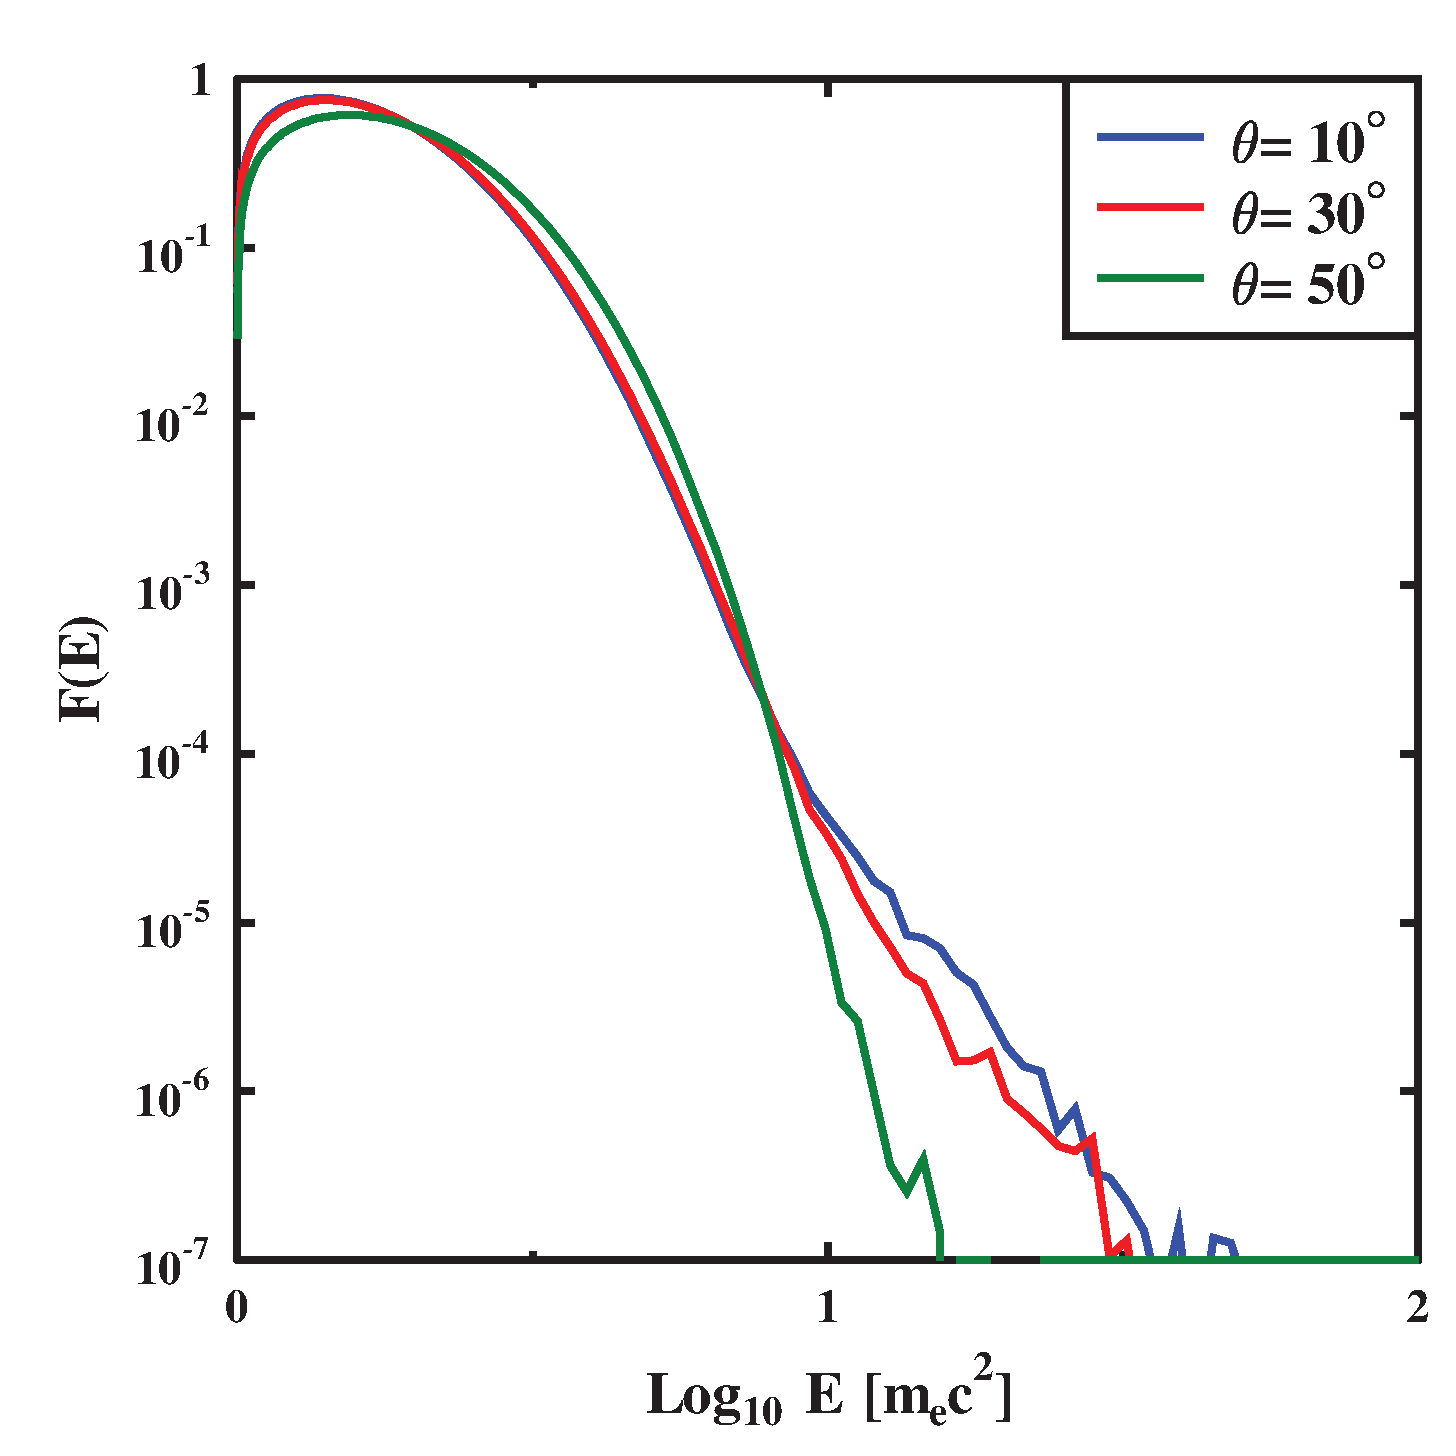
\includegraphics[width=10.5 cm]{compareelectrons2.eps} 
	\caption{Функция распределения электронов за фронтом ударной волны при следующих параметрах: скорость потока \mbox{$v = 0.3~c,$} , магнетизация $\sigma = 0.0002$ при нескольких углах наклона.}
	\label{compareelectrons}
\end{figure}
 
Для дальнейшего моделирования излучения использовалась функция распределения, полученная для угла $\theta = 30^\circ$ градусов (квазипараллельная ударная волна).
 
Из результатов моделирования можно извлечь параметры полученного распределения электронов. За фронтом ударной волны функция распределения электронов имеет сложный вид, но можно выделить две основных компоненты - тепловой пик и степенной хвост на высоких энергиях.
На низких энергиях ($\displaystyle E < 5 m_e c^2$) мы аппроксимируем фунцию распределения с помощью распределения Максвелла-Юттнера, итеративным процессом минимизируя функционал $\displaystyle f(T) = \int_{m_e c^{2}}^{5 m_e c^{2}} (F(E) - F_{mj}(E,T))^{2}dE$, где $\displaystyle F(E)$ функция распределения полученная из моделирования, $\displaystyle F_{mj}(E,T)$ - распределение Максвелла-Юттнера. Таким образом определяется температура, соответствующая тепловому пику. Для высоких энергий ($\displaystyle 20~m_e c^{2} < E < 50~m_e c^{2}$) мы используем линейную регрессию в дважды логарифмических координатах для определения спектрального индекса $p$. Функция распределения электронов за фронтом ударной волны (от 2000 до 5000 ячеек за фронтом) в момент времени $\displaystyle t$ = 70,000~$\omega_{e}^{-1}$ при начальных параметрах $\displaystyle\sigma = 0.0002$, $\theta = 30^\circ$ и ее аппроксимации с \textcolor{red}{температурой $\displaystyle T_e = 5\times 10^{10}$~K} и спектральным индексом $\displaystyle p = 3.6$ изображены на рисунке ~\ref{electrons}.
\begin{figure}
		\centering
		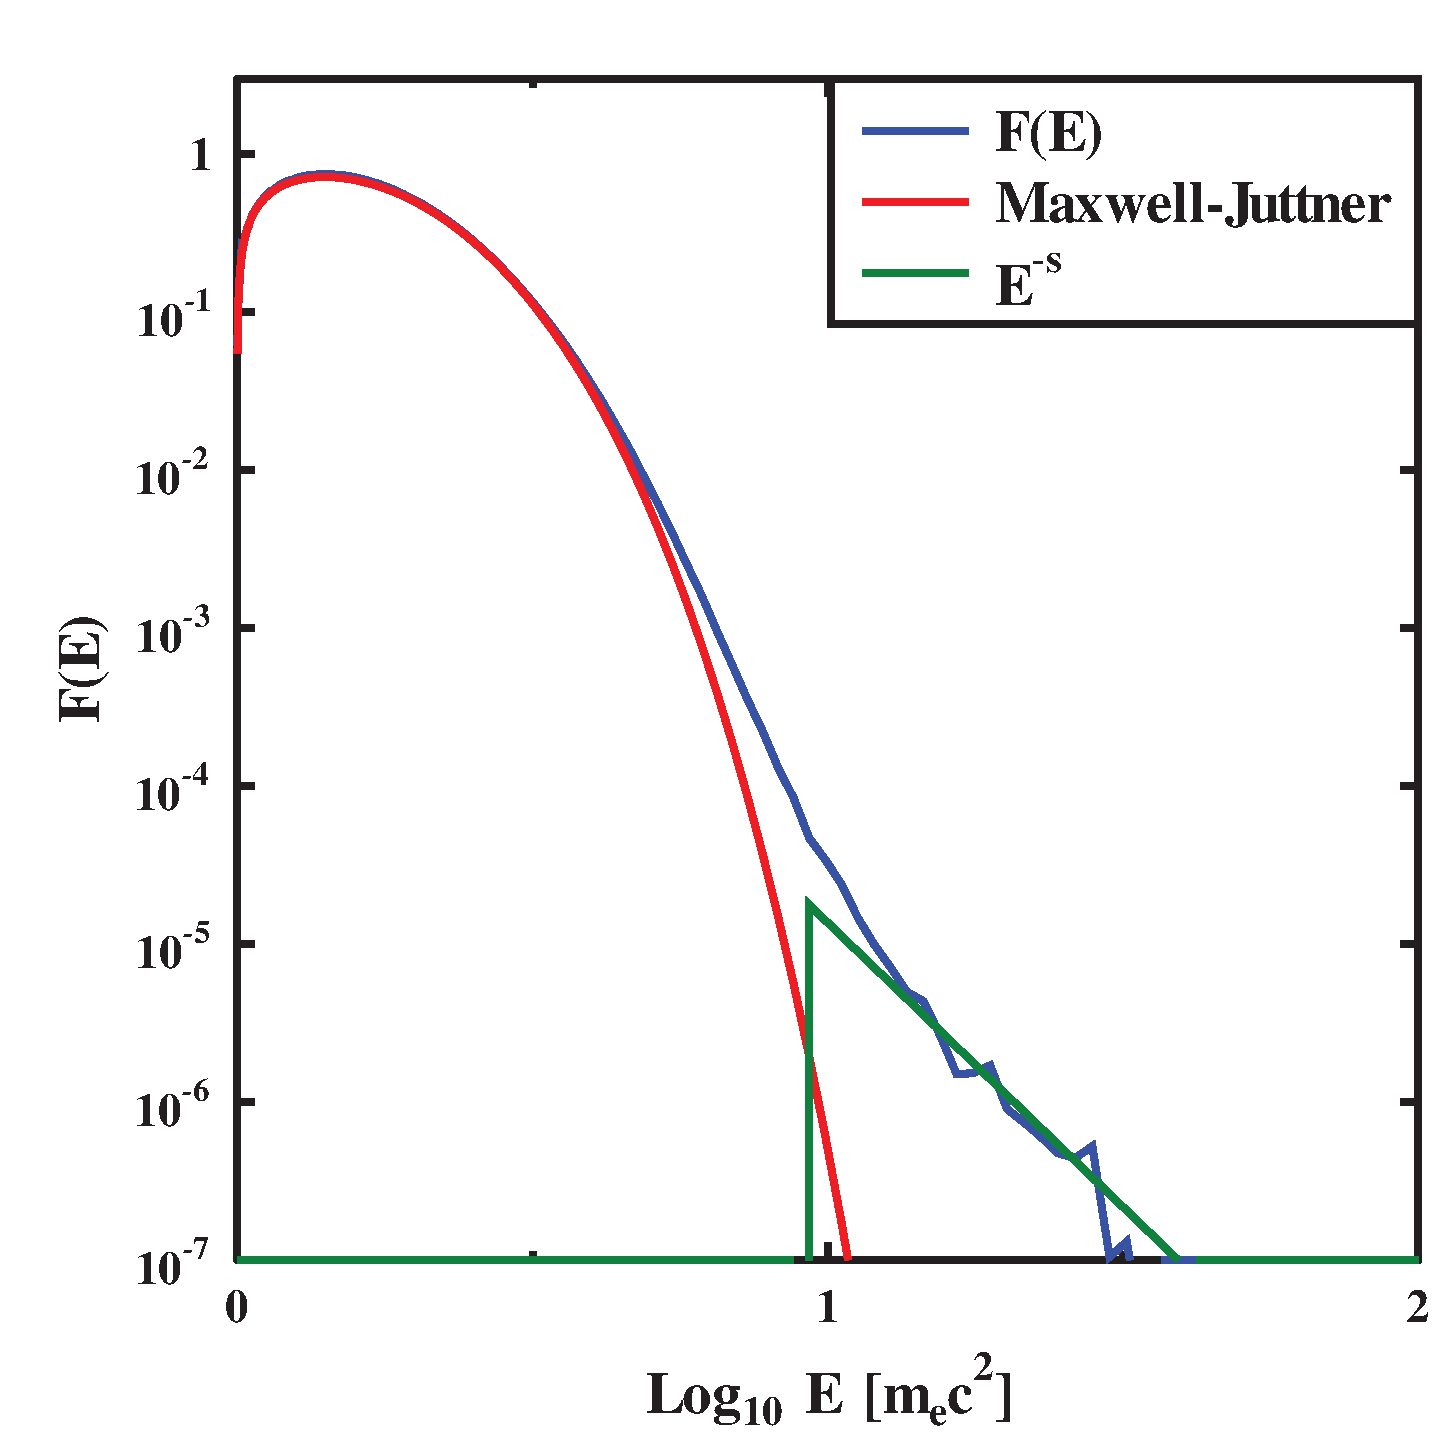
\includegraphics[width=10.5 cm]{electrons.eps} 
		\caption{Функция распределения электронов за фронтом ударной волны при начальных параметрах $v = 0.3~c,$ $\sigma = 2\times10^{-4}$ и $\theta = 30^{\circ}$.}
		\label{electrons}
	\end{figure}

\section{Расчёт излучения}




\section{Результаты}




\FloatBarrier
\section{Заключение}
 

Получены следующие результаты:
\begin{enumerate}
\item 
\item 
\end{enumerate}


\clearpage			% Глава 1. Моделирование излучения FBOT.
%\chapter{Классификация гамма-всплесков, зарегистрированных в эксперименте Конус-Винд}\label{KW_GRB_classification}

\section{Введение}
Первым свидетельством наличия двух классов всплесков было обнаружение их бимодального 
распределения по длительности~\citep{Mazets_1981_part_1,Norris_1984,Kouveliotou_1993,Aptekar_1998}. 
В работе \citep{Kouveliotou_1993} были введены две меры длительности $T_{50}$ и $T_{90}$, 
которые соответствуют временам накопления 50\% и 90\% от суммарного числа отсчётов 
всплеска (интервалы от 25\% до 75\% и от 5\% до 95\% отсчётов, соответственно), 
и определена граница между длинными и короткими всплесками $T_{90}=2$~с 
на основе локального минимума бимодального распределения. 
В работе \citep{McBreen_1994} обсуждается, что распределение всплесков по 
длительности $T_{90}$ хорошо описывается суммой двух логнормальных компонент. 
Более детальный анализ распределения по $T_{90}$ всплесков из третьего каталога 
эксперимента BATSE~\citep{Horvath_2002} показал, что распределение 
хорошо аппроксимируется тремя логнормальными компонентами. 
Третья компонента располагалась между короткими и длинными всплесками, 
что свидетельствовало о наличие третьего класса всплесков с промежуточной длительностью.
Доля промежуточных всплесков составила 6\%. 

Систематические ошибки величин $T_{50}$ и $T_{90}$, которые искажают наблюдаемое 
распределение всплесков, были рассмотрены в работе~\citep{Norris_and_Bonnel_2006ApJ} 
на примере всплесков, зарегистрированных в эксперименте \textit{CGRO}-BATSE~\citep{Fishman_1992NASCP3137}. 
Было показано, что как минимум четыре фактора влияют на измеренное значение длительности 
всплеска и размывают границы между классами коротких и длинных всплесков: 
(1)~различие в отношении сигнал-шум (S/N) между самым интенсивным и самым слабым 
всплеском  при условии, что эти всплески не отличаются по другим параметрам, 
приводит к различию их длительностей $T_{90}$ в $\sim 2$~раза~\citep{Bonnell_1997}; 
(2)~длительность космологически удалённых длинных всплесков (с красными смещениями источников 
$z \sim 2 \textrm{--}10$) увеличивается в 2--5 раз по сравнению со всплесками, 
пришедшими с $z=1$, в это же время поправка длительности 
для коротких всплесков не превышает двух раз, так как их источники в основном 
расположены на $z<1$ (этот фактор увеличивает обособленность распределений 
коротких и длинных всплесков); (3)~эффект зависимости длительности отдельных импульсов 
всплесков от энергии $\propto E^{-0.35}$~\citep{Fenimore_1995}, а так же модификация 
спектра за счёт космологического расширения приводит к зависимости длительности 
всплеска от энергетического диапазона наблюдений; (4)~распределение по длительностям 
обрезано со стороны коротких всплесков вследствие наблюдательной селекции триггерного 
алгоритма. 

Кроме $T_{50}$ и $T_{90}$ была предложена и другая мера длительности~--- время 
эмиссии~\citep{Mitrofanov_1999}, которая вычисляется как суммарная длительность 
бинов временной истории, в которых интенсивность излучения превышает заданный 
уровень от пиковой интенсивности. Этот уровень задается таким образом, чтобы 
суммарное число отсчетов в бинах составляло заданную долю от общего числа отсчётов 
всплеска (использовались уровни 30\% и 50\%, соответствующие меры длительности 
были обозначены $\tau_{30}$ и $\tau_{50}$). Было показано, что данная мера 
длительности гораздо менее чувствительна и к отношению сигнал-шум и к количеству 
импульсов во всплеске, разделенных значительным промежутком фона, так как этот 
промежуток не входит, по определению, в определяемое время эмиссии. Ясно, однако, 
что эта мера чувствительна к временному разрешению. Распределения всплесков 
по $\tau_{30}$ и $\tau_{50}$  также являются бимодальными. Эти меры длительности 
не получили широкого распространения, поэтому классификация всплесков 
на их основе в данной работе не рассматривается. 

Короткие и длинные всплески, в среднем, отличаются жёсткостью спектра.
В работе \citep{Kouveliotou_1993} было обнаружено, что короткие всплески BATSE, в 
среднем, имеют большую жёсткость ($\rmn{HR}_{32}$), чем длинные, где $\rmn{HR}_{32}$ определялась 
как отношение числа отсчетов, накопленных за $T_{90}$ в энергетических 
диапазонах 100--300~кэВ и 50--100~кэВ (диапазоны 3 и 2) эксперимента \textit{CGRO}-BATSE. 
Однако, в последующих работах было отмечено, что жёсткость не является обязательной чертой 
коротких всплесков~\citep[см., например,][]{Sakamoto_2006_proc, Norris_and_Bonnel_2006ApJ}. 

На основе распределения на плоскости жёсткость-длительность также был обнаружен 
третий класс всплесков ~\citep{Mukherjee_1998, Hakkila_2000}. Анализ влияния 
систематических эффектов на наличие третьего класса всплесков был проведён 
в~\citep{Hakkila_2003}. Авторы показали, что третий класс всплесков не является 
физическим и может являться следствием селекции триггерного алгоритма. Также было 
показано, что сам по себе эффект зависимости длительности от яркости 
всплеска~\citep{Bonnell_1997} не может привести к появлению третьего класса всплесков. 
Однако, в последующей работе~\citep{Horvath_2006} были приведены доводы в пользу 
реальности третьего класса всплесков и исследовалось количество и значимость 
классов всплесков на основе параметров распределения на плоскости 
$\log T_{90}$--$\log \rmn{HR}_{32}$ для 1956 всплесков, зарегистрированных 
в эксперименте BATSE. При этом распределение аппроксимировалось 
суммой двумерных нормальных распределений. Было установлено, что распределение 
наилучшим образом описывается тремя компонентами (классами). При этом доля всплесков 
из класса с промежуточной длительностью составляет 10--15\%. Также было показано, что поправка набора 
всплесков на селекцию триггерного алгоритма сохраняет полученное разделение на классы. 
Аналогичный метод был применен к 222 всплескам \textit{Swift}-BAT~\citep{Horvath_2010}, 
при этом также было обнаружено три класса всплесков. При этом доля промежуточного 
класса всплесков составила~30\%.

Помимо жесткости и длительности, еще одним параметром для классификации всплесков 
может служить спектральная задержка. Этот параметр характеризует запаздывание 
излучения в более мягком диапазоне по отношению к излучению в более жестком диапазоне. 
Значение задержки ($\tau_\rmn{lag}$) соответствует положению  максимума 
кросскорреляционной функции временных историй в двух энергетических диапазонах~\citep{Norris_2000}. 
Анализ спектральных задержек коротких всплесков BATSE и \textit{Swift}-BAT показал, 
что они распределены вблизи нуля с разбросом 
порядка 25~мс \citep{Norris_and_Bonnel_2006ApJ, Norris_2011ApJ}. В то же время длинные 
всплески могут иметь значительные задержки. Идея о том, что различие спектральных 
задержек длинных и коротких всплесков отражает различие физических свойств источников 
всплесков, была выдвинута в работе~\citep{Gehrels_2006_Nature}.

%Существует несколько моделей, объясняющих появление спектральной задержки. 
%В работе~\citep{Ioka_and_Nakamura_2001} появление задержки объясняется, тем что 
%узкий джет наблюдается под разными углами для разных всплесков. Большая задержка 
%соответствует большему углу наблюдения относительно оси джета. 
%Авторы работы~\citep{Schaefer_2004_lag} считают, что спектральная задержка в 
%каждом импульсе всплеска характеризует время потери энергии излучающими частицами.

После начала эры многоволновых наблюдений гамма-всплесков стало возможным 
классифицировать всплески на основании параметров послесвечений и родительских галактик. 
В работах~\citep{Zhang_2006, Zhang_2007, Zhang_2009} была предложена схема классификации всплесков, 
основанная на этих параметрах, на физические типы: I и~II. Считается, что всплески типа~I, 
генерируются при слиянии компактных объектов, а всплески типа~II образуются 
при коллапсе молодых массивных звёзд. В работе~\citep{Zhang_2009} было показано, 
что всплески типа II на плоскости жёсткость-длительность располагаются в области 
длинных/мягких всплесков, при этом всплески типа~I~--- в области коротких/жестких событий. 
Авторы также отмечают, что всплески типа I обладают незначительной спектральной задержкой.

Неоднозначность соответствия коротких всплесков и всплесков типа~I связана, в том числе, с 
существованием коротких гамма-всплесков, сопровождающихся слабым сравнительно мягким 
излучением в гамма-диапазоне, длящимся десятки секунд после начального короткого импульса. 
Это явление получило название продленного излучения (EE).
Впервые этот класс всплесков был обнаружен в данных BATSE~\citep{Burenin_2000AstL} и 
Конус~\citep{Mazets_2002astro_ph}. В работе~\cite{Frederiks_2004ASPC} 
было обнаружено 11 всплесков с продлённым излучением среди 125 коротких гамма-всплесков KW. 
Для оставшихся всплесков был обнаружен избыток излучения на интервале 5--100~с в сумме временных 
профилей с вычтенным фоном. Такой же избыток был выявлен в данных 
BATSE~\citep{Lazzati_2001AandA, Connaughton_2002ApJ}, \textit{BeppoSAX}-GRBM~\citep{Montanari_2005ApJ} и 
\textit{INTEGRAL}-SPI-ACS~\citep{Minaev_2010AstL}. 
%написать про всплески с EE на BAT и GBM
Основную сложность представляет разделение коротких всплесков с EE 
и длинных всплесков. Авторы работы~\citep{Norris_and_Bonnel_2006ApJ} использовали визуальные признаки 
для выделения коротких всплесков с продлённым излучением: длительность начального 
импульса $T_{90}<2$~с, отсутствие заметной спектральной эволюции в начальном 
импульсе и EE. Авторы обнаружили в данных BATSE 8 всплесков, 
удовлетворяющих этим критериям, и показали, что их спектральные задержки близки к нулю. 
Также в работе отмечается наличие у некоторых всплесков интервала с практически нулевой интенсивностью излучения 
между начальным импульсом и продлённым излучением. Сравнение интенсивностей продлённого 
излучения для этих 8 всплесков и интенсивности излучения, обнаруженного в 
суммарном временном профиле в работе~\citep{Lazzati_2001AandA}, показывает, 
что динамический диапазон интенсивности продлённого излучения составляет $\sim 10^4$, 
так же как и динамический диапазон отношения интенсивности начального импульса и продлённого излучения.
В работе~\citep{Norris_2010ApJ} на основе 12 всплесков с продлённым излучением, зарегистрированных 
\textit{Swift}-BAT, был оценен физический порог отношения интенсивностей продлённого излучения 
и начального пика как единицы $\times 10^3$ и было показано, что для начальных импульсов 
всплесков без продлённого излучения характерны в $\sim 2\textrm{--}3$ раза меньшие длительности
 по сравнению с всплесками с EE, также всплески без продлённого излучения 
имеют меньшее число пиков в начальном импульсе.

Различие природы источников коротких гамма-всплесков с продлённым излучением и 
без него в настоящее время не подтверждено. В работе~\citep{Troja_2008MNRAS} 
было установлено, что смещения относительно центра родительской галактики 
коротких всплесков с продлённым излучением в среднем меньше, чем для всплесков без него: 
единицы и десятки килопарсек, соответственно. 
Исследование~\citep{Fong_2010ApJ} с использованием данных наблюдений 
телескопа \textit{Hubble Space Telescope} опровергло этот результат.

В данной главе анализируются временные истории всплесков, зарегистрированных в 
эксперименте Конус-Винд. Всплески классифицируются на основе длительности, жесткости и 
спектральной задержки, и определяется набор коротких всплесков для дальнейшей локализации и спектрального анализа. 
При этом обсуждается принадлежность исследуемых всплесков к типам~I и~II. 
В разделе~\ref{sec:GRB_sample} приводится описание использованного набора всплесков. 
В разделе~\ref{sec:Durations} рассматривается распределение всплесков по длительности, 
определяется граница между длинными и короткими всплесками на основе 
длительности $T_{50}$ и определяется итоговый набор коротких всплесков. 
В разделе~\ref{sec:Hardness} рассматриваются жесткости всплесков и производится 
классификация всплесков на основе соотношения жёсткость-длительность. 
В разделе~\ref{sec:Lags} анализируются спектральные задержки коротких всплесков. 
Сравнение классификации на физические типы~I и~II и классификации на основе жесткости, 
длительности и спектральной задержки приведено в разделе~\ref{sec:Phys_Classification}. 
Обобщение и обсуждение результатов приведено в разделе~\ref{sec:Conclision}.  

\section{Набор всплесков}\label{sec:GRB_sample}
За период с ноября 1994~г. по декабрь 2010~г. KW зарегистрировал 2008 гамма-всплесков 
в триггерном режиме. Среди них 69 всплесков содержат сбои, представляющие собой 
промежутки в данных во время всплеска, или значительные флуктуации фона, 
накладывающиеся на всплеск. Всего 1939 всплесков без сбоев.

Для вычисления параметров временных историй использовалась 
сшивка фоновой и триггерной записи. Длительность всплесков, у которых значительная 
часть события лежит в бине фоновой записи, предшествующем триггерной записи, может быть 
искажена из-за низкого разрешения фоновой записи. Из дальнейшего рассмотрения 
было исключено 105 таких событий. Таким образом, для анализа использовались временные 
истории 1834 гамма-всплеска. 

\section{Длительности}\label{sec:Durations}
Для вычисления длительностей мы использовали сумму временных историй всплеска 
в энергетических диапазонах G2 и G3. Такой выбор обоснован тем, что  пиковая 
энергия $E F_{E}$ спектра ($E_\rmn{p}$) абсолютного большинства всплесков лежит в 
диапазоне $E_\rmn{p}>80$~кэВ, и, следовательно, отсчёты, соответствующие основному энерговыделению 
во всплеске, регистрируются в диапазонах G2 и G3. Фон в G2 и G3 стабилен на более 
длительных интервалах времени, чем в G1. Это позволяет с гораздо меньшей вероятностью 
неверно определять начало и конец всплеска из-за флуктуаций фона. Также в диапазон G1 
может попадать начало рентгеновского послесвечения, учёт которого исказит 
длительность начального импульса всплеска.

Уровни фона для вычисления длительностей определялись по методике, описанной в 
разделе~\ref{sec:Bg_rate} Главы~\ref{KW_description}. 
В результате, из всего набора 1834 всплесков у 96\% всплесков длительность 
интервала для определения фона составила 750~с и только у $<1$\% всплесков длительность этого 
интервала составила 30--100~c.

\subsection{Автоматическая процедура определения длительности}
Основной задачей при вычислении любой меры длительности является определение момента 
начала и конца всплеска. В работе~\citep{Koshut_1996}, описывающей методику вычисления 
длительностей $T_{90}$ и $T_{50}$  для второго каталога BATSE, моменты начала и 
конца всплеска $t_{0}$ и $t_{100}$ определялись визуально на основании интеграла 
от временной истории с вычтенным фоном всплеска, где $t_{x}$ соответствует времени накопления заданной 
доли $x$  (0\%, 5\%, \dots, 100\%) от полного числа отсчётов всплеска. 
В работе~\citep{Bonnell_1997} использовалась автоматическая процедура поиска 
$t_{0}$ и $t_{100}$, которая заключалась в поиске положительной флуктуации числа 
отсчетов с вычетом фона со значимостью от $3\sigma$ до $6\sigma$ на временных 
масштабах от 0.5~с до 16~с в диапазоне~$>25$~кэВ.
% что для Swift-BAT и Fermi-GBM?  

Для вычисления длительности всплесков KW использовалась автоматическая 
процедура поиска начала и конца всплеска. Поиск производился на интервале от 
$T_0-250$~с до $T_0+230$~с (конец триггерной записи), где $T_0$~--- время триггера KW. 
Для некоторых всплесков границы интервала вычисления длительности отличались от указанных, 
к примеру, в случае присутствия солнечной вспышки в данных. Для поиска начала 
всплеска производился поиск положительной флуктуации числа отсчетов с вычетом 
фона на заданном уровне значимости. При этом поиск превышения производился на 
интервале с длительностью от временного разрешения текущего участка записи до 100~с. 
Началом всплеска $t_0$ считается начало интервала, на котором было обнаружено превышение, 
если вероятность его случайного обнаружения была меньше пороговой. 
Иллюстрация алгоритма поиска начала всплеска приведена на рис.~\ref{fig:T100_calculation}.
Времена начала интервалов поиска превышения брались последовательно, начиная от $T_0-250$~с. 
Конец всплеска~--- $t_{100}$ определяется аналогичного, при этом поиск ведётся в 
обратном направлении по времени, начиная от $T_0 + 230$~с. Длительности всплесков 
вычислялись для порогов, соответствующих вероятности случайного превышения 
значений $4\sigma$, $5\sigma$ и $6\sigma$ для распределения Гаусса. При этом на 
интервалах, где число отсчётов от фона меньше 20, для вычисления вероятности 
случайного превышения использовалась статистика Пуассона. Значения $T_{90}$ и $T_{50}$ 
и их ошибки определялись методом, описанном в работе~\citep{Koshut_1996}. 


\begin{figure}[h]
  \begin{minipage}[h]{0.5\textwidth}
    \center{\includegraphics[width=1.0\textwidth]{gDurStartRU.eps} \\ а)}
  \end{minipage}
  \hfill
  \begin{minipage}[h]{0.5\textwidth}
    \center{\includegraphics[width=1.0\textwidth]{gDurT5RU.eps} \\ б)}
  \end{minipage}  
  \caption{
  (а) Иллюстрация определения времени начала всплеска $t_0$ для GRB20031214\_T36655. 
  Сплошная линия~--- интегральное число отсчетов всплеска с вычетом фона. 
  Число отсчётов $N_\rmn{acc}$ (горизонтальные штриховые линии), 
  накопленное на интервале $\Delta T_\rmn{acc}$ (вертикальные штриховые линии), 
  соответствует превышению $5\sigma$ над фоном. Уровень $1\sigma$ относительно интегрального 
  числа отсчётов на момент $t_0$  изображен горизонтальной штрихпунктирной линией. 
  Горизонтальная точечная линия обозначает нулевой уровень.
  (б) Иллюстрация определения начала интервала $T_{90}$ ($t_5$) для того же всплеска.
  Число отсчётов, соответствующие 5\% от общего числа отсчётов $N_\rmn{tot}$ 
  обозначено горизонтальными штриховыми линиями, время начала всплеска $t_0$ и время $t_5$ 
  обозначены вертикальными штриховыми линиями. \label{fig:T100_calculation} }
\end{figure}

\subsection{Распределения по длительностям}
Для 1834 всплесков KW были построены гистограммы распределений всплесков по $T_{90}$ и $T_{50}$ 
для порогов значимости поиска начала и конца всплеска $4\sigma$, $5\sigma$ и $6\sigma$. 

Распределения  аппроксимировались методом минимизации $\chi^2$ суммой двух логнормальных распределений
\begin{equation}
f(x) = \sum_{l=1}^{2} A_l f_l(x) \mbox{ ,}
\end{equation}
где
\begin{equation}
f_l(x) = \frac{1}{w_l \sqrt{\pi/2}} \exp\left(\frac{-2(x-x_{cl})^2}{w_l^2}\right) \mbox{ ,}
\end{equation}
с параметрами $A_l$~--- площадь под распределением, $w=2\sigma$~--- ширина, $x_{cl}$~--- среднее значение и 
$x=\log T$. При этом число всплесков в бине по модели равно  интегралу от аппроксимирующей функции в границах бина. 

Доверительные интервалы параметров распределения на уровне 68\% вычислялись 
методом Mонте-Карло для 1000 реализаций распределения. При этом значение в каждом 
бине распределения разыгрывалось как пуассоновская случайной величиной со средним, равным 
числу отсчётов в соответствующем бине исходного распределения. Полученный набор 
значений каждого параметра распределения сортировался по возрастанию. В качестве нижней и верхней 
границы доверительного интервала на уровне 68\% из этого отсортированного массива 
параметров брались значения с индексами 160 и 840, соответственно. 
В качестве значения параметра бралась медиана распределения.

Из-за эффектов селекции число очень коротких всплесков ($T_{90} \lesssim 100$~мс) и 
число длинных всплесков ($T_{90} \gtrsim 200$~с) в наборе KW недооценено. Так же неверно 
считать ошибки числа отсчётов в бине гауссовыми при числе отсчётов $<10$, поэтому 
бины с $\log T_{90} \leq -1.2$ ($T_{90} \leq 0.063$~с) и $\log T_{90} \geq 2.4$ ($T_{90} \geq 251$~с) 
не учитывались при аппроксимации гистограммы распределения по $T_{90}$,  для аппроксимации 
использовалось 18 бинов. При аппроксимации гистограммы распределения по $T_{50}$ игнорировались 
бины c $\log T_{50} \leq -1.8$ ($T_{50} \leq 0.016$~с) и  $\log T_{50} \geq 2.0$ 
($T_{50} \geq 100$~с), для аппроксимации использовалось 19 бинов.

Параметры распределений представлены в таблицах~\ref{tab:T90_distr} и~\ref{tab:T50_distr}. 
Из представленных результатов видно, что при изменении порога от $4\sigma$ до $6\sigma$ 
параметры распределения по $T_{50}$ и $T_{90}$ для полного набора 1834 всплесков изменяются. 
Распределение длинных всплесков смещается в сторону меньших длительностей, такое же смещение, 
но в меньшей степени, наблюдается для распределение коротких всплесков. 
При этом изменение параметров распределения по $T_{90}$ гораздо существенней, 
чем для распределения по $T_{50}$, см. таб.~\ref{tab:Txx_vs_thd},
где $T_{\rmn{int}}$ соответствует пересечению распределений и 
$\delta T =|T_{4\sigma}-T_{6\sigma}| / T_{4\sigma}$. 
Так как вариации параметров распределения по $T_{50}$ существенно меньше, 
чем для распределения по $T_{90}$ для классификации всплесков на основе длительностей 
мы выбрали величину~$T_{50}$. 

\input{tables/duration_vs_thd}

Вследствие наблюдательной селекции триггерной системы по отношению сигнал-шум 
наш набор всплесков неоднороден. Как видно из диаграммы $T_{50}$--$\rmn{S/N}$~(рис.~\ref{img:SNvsT50}) 
в наборе отсутствуют всплески с отношением сигнал-шум $\rmn{S/N} < 10$ и $T_{50} \lesssim 100$~мс. 
Здесь S/N определено как отношение числа отсчётов от источника к стандартному отклонению 
числа отсчётов фона на интервале 64~мс с максимальной скоростью счёта. 
Для дальнейшего рассмотрения был выбран однородный набор всплесков с $\rmn{S/N}\geq 10$, 
который содержит 1168 всплесков. 
Результаты аппроксимации распределений набора по $T_{50}$ и $T_{90}$ приведены в 
таблицах \ref{tab:T90_distr} и~\ref{tab:T50_distr}, и на рис.~\ref{img:T90andT50s5}. 
Относительные изменения параметров скорректированных распределений при изменении 
порога от $4\sigma$ до $6\sigma$ приведены в таб.~\ref{tab:Txx_vs_thd}. 

В качестве порога значимости был выбран уровень $5\sigma$ так как было замечено, 
что при пороге $4\sigma$ в качестве начала и конца всплеска часто выбираются 
флуктуации фона или эпизоды излучения транзиентов, не относящиеся ко всплеску  
(установить отношение подобных слабых эпизодов к триггерному всплеску в 
большинстве случаев не представляется возможным). При пороге $6\sigma$ часто 
игнорируется <<хвост>>, непосредственно прилегающий к основному пику, тем самым полное 
число отсчетов во всплеске может недооцениваться на величину до $\sim 70$\%.
Такая ситуация возможна, к примеру, для коротких всплесков с продлённым излучением.

В качестве границы между длинными и короткими всплесками была выбрана точка пересечения 
двух логнормальных распределений по $T_{50}$ для порога значимости $5\sigma$ 
набора 1168 всплесков $T_{50\rmn{,int}} = 0.6$~с. 

Для указанного распределения и границы между длинными и короткими всплесками 
можно оценить долю <<засорения>>\ набора коротких всплесков длинными и наоборот. 
Доля <<засорения>>\ набора коротких всплесков длинными равна отношению интеграла 
от распределения длинных всплесков и интеграла от распределения коротких всплесков 
на интервале $-\infty$ до $T_{50\rmn{int}}$) и составляет $\approx 7$\%. 
При этом доля <<засорения>>\ длинных всплесков короткими составляет~$\approx 2$\%.          

Границы диапазонов KW менялись со временем, что могло внести систематический 
сдвиг в длительности всплесков, зарегистрированных в различные периоды, и 
привести к изменению со временем границы между длинными и короткими всплесками. 
Для анализа дрейфа границы между длинными и короткими всплесками набор 1168 
всплесков был разделён на три поднабора: 583 GRBs ноябрь 1994~-- май 2003; 
585 GRBs июнь 2003~-- декабрь 2010; 582 GRBs  май 1999~-- январь 2007. 
Полученные для поднаборов границы $T_{50\rmn{int}}$ равны: 
$0.41_{-0.09}^{+0.19}$~c, 
$0.74_{-0.16}^{+0.22}$~c и 
$0.62_{-0.17}^{+0.28}$~c, соответственно. 
Наблюдаемый дрейф границы лежит в пределах $1\sigma$ интервала для границы $T_{50\rmn{int}} = 0.6$~с, 
полученной с использованием полного набора всплесков.

\begin{figure} [h] 
  \center
  \includegraphics [width=0.75\textwidth] {gSNvsT50_ru}
  \caption[Соотношение S/N--$T_{50}$]{Соотношение S/N--$T_{50}$ для 1834 всплесков. 
  Пунктирная линия соответствует $\rmn{S/N}=10$. Штрихованная область наиболее подвержена 
  селекции триггерного алгоритма. Отношение сигнал-шум $\rmn{S/N}\geq 10$ имеют 1168 всплесков.} 
  \label{img:SNvsT50}  
\end{figure}

\begin{figure}[h]
  \begin{minipage}[h]{0.5\textwidth}
    \center{\includegraphics[width=1.0\textwidth]{dT90s5simple} \\ а)}
  \end{minipage}
  \hfill
  \begin{minipage}[h]{0.5\textwidth}
    \center{\includegraphics[width=1.0\textwidth]{dT90s5simple_SN10} \\ б)}
  \end{minipage}
  \vfill
  \begin{minipage}[h]{0.5\textwidth}
    \center{\includegraphics[width=1.0\textwidth]{dT50s5simple} \\ в)}
  \end{minipage}
  \hfill
  \begin{minipage}[h]{0.5\textwidth}
    \center{\includegraphics[width=1.0\textwidth]{dT50s5simple_SN10} \\ г)}
  \end{minipage}
  \caption[Распределения 1834 и 1168 всплесков с $\rmn{S/N}\geq 10$ по $T_{90}$ и~$T_{50}$]
  {Распределения 1834 и 1168 всплесков с $\rmn{S/N}\geq 10$ по $T_{90}$~(а и б, соответственно) и 
  $T_{50}$ (в и г, соответственно) для порога $5\sigma$ (непрерывная гистограмма), 
  игнорированные при аппроксимации бины гисторграммы показаны пунктиром. 
  Аппроксимация распределения суммой двух логнормальных распределений  показана 
  непрерывной линией, распределение коротких и длинных всплесков показаны 
  штрихпунктирными линиями.  Вертикальные штриховые лини обозначают средние значения 
  распределений коротких и длинных всплесков и точку их пересечения. 
  На нижней панели каждого рисунка показаны невязки аппроксимации.}
  \label{img:T90andT50s5}  
\end{figure}

\begin{landscape}
\input{tables/duration_tables_mc_diss}
\end{landscape}

\subsection{Сравнение длительностей определенных по данным BATSE и KW}
Среди 1939 всплесков KW без сбоев 267 всплесков наблюдались BATSE. 
Соотношение длительностей $T_{50}$ и $T_{90}$, вычисленных по данным BATSE~\citep{Paciesas_1999} 
и KW, изображено на рис.~\ref{img:T90andT50_KWvsBATSE}.

Большинство всплесков имеют б\'{о}льшую длительность по данным BATSE, 
в особенности $T_{90}$ по сравнению с KW, что связано с большей  эффективной площадью детекторов 
BATSE $\sim 10^3$~см$^2$ против $(0.80\textrm{--}1.6)\times 10^2$~см$^2$ у KW. 
Другим фактором является то, что длительность всплесков BATSE определяется в 
диапазоне $>25$~кэВ, что позволяет учитывать продолжительные мягкие хвосты всплесков. 
Более редкой ситуацией является существенное превышение длительностей по данным KW, 
наблюдаемое в 10 всплесках. Шесть всплесков имеют плавное спадание/нарастание интенсивности, 
которое не было учтено при вычислении  длительностей по данным BATSE, возможно, 
из-за недостаточно точной аппроксимации фона. В трех всплесках по данным KW
в интервал $T_{90}$ попадает слабый импульс, отделенный от основного пика. 
При этом эклиптические широты основного пика и слабого импульса согласуются, 
что позволяет отнести их к одному источнику. Во всплеске GRB~950904, 
$T_{0\rmn{,BATSE}} = 52777$~s~UT ($T_{90\rmn{,KW}} = 99 \pm 4$~с, $T_{90\rmn{,BATSE}} = 11.1\pm 1.8$~с) 
длительности BATSE даны для второго импульса, так как в~\citep{Hurley_2005} полагается, 
что два импульса являются различными всплесками.

Среди общих всплесков KW и BATSE 46 имеют $T_{50\rmn{KW}} \leq 0.6$~с, 
из них 9 входят в набор 105 всплесков с искаженной длительностью (см.~Раздел~\ref{sec:GRB_sample}). 
Из оставшихся 37, 8 имеют $T_{90\rmn{BATSE}} > 2$~с, 
из них один является короткими всплеском с продлённым излучением. Таким образом, 
засорение нашего списка длинными всплесками, связанное с низким S/N всплесков KW
по сравнению с BATSE, составляет 19\% (=7/37). % без учета всплесков с продлённым излучением. 
Ранее в работе~\citep{Ofek_2007ApJ} была получена доля 
<<засорения>> коротких всплесков KW длинными $\approx 60$\%. В этой работе
длительность всплесков в данных KW оценивалась визуально, что могло 
стать причиной получения высокой доли засорения. 

\begin{figure}[h]
  \begin{minipage}[h]{0.5\textwidth}
    \center{\includegraphics[width=1.0\textwidth]{gT90_KWvsBATSE_ru} \\ а)}
  \end{minipage}
  \hfill
  \begin{minipage}[h]{0.5\textwidth}
    \center{\includegraphics[width=1.0\textwidth]{gT50_KWvsBATSE_ru} \\ б)}
  \end{minipage}
  \caption{Соотношение длительностей $T_{90}$~(a) и $T_{50}$~(б), определённых по 
  данным BATSE и KW для 267 гамма-всплесков.}
  \label{img:T90andT50_KWvsBATSE}  
\end{figure}

\subsection{Набор коротких всплесков}
Набор из 1834 всплесков KW содержит 277 событий с $T_{50} \leq 0.6$~с.    %<-- число 277 проверено
Среди них было обнаружено: пять очевидно длинных всплесков, в которых $T_{50}$ 
% (ID = 1122, 2196, 2922, 2184) и ID=1228 $T_{90} = 8$~с в данных SAX
определялось наиболее сильным импульсом, при этом полная длительность всплеска была 
значительно больше 2~с; и 12 кандидатов в короткие всплески с продлённым излучением.
Визуальный анализ показал, что среди 69 всплесков со сбоями пять имеют $T_{50} \leq 0.6$~с, 
эти всплески были включены в итоговый набор. 
% ID = 243, 704, 882 (солн. вспышка в данных), 934, 3319 (пропущен ранее)
Таким образом, набор коротких всплесков KW содержит 265 событий без продлённого излучения.

Кроме того, было обнаружено 19 кандидатов во всплески с продлённым излучением среди всплесков с $T_{50} > 0.6$~с. 
К этому типу всплесков были отнесены события, имеющие короткий начальный импульс с $T_{50} \leq 0.6$~с, 
за которым следует эпизод излучения, не содержащий импульсов с заметной спектральной эволюцией. 
В некоторых случаях начальный пик и продлённое излучение были разделены интервалом, 
на котором интенсивность излучения мала. Таким образом, полученный набор коротких всплесков с 
продлённым излучением насчитывает 31 событие.

Объединённый набор коротких всплесков с учётом всплесков с продлённым излучением 
содержит 296 событий.
\FloatBarrier

\section{Жесткости}\label{sec:Hardness}
Для анализа спектральных различий всплесков использовалось две величины: интегральная 
жёсткость ($\rmn{HR}_{32}$)~--- отношение числа отсчетов, накопленных в каналах G3 и G2 
за интервал $T_{100}$ и пиковая жёсткость ($\rmn{HR}_{32\rmn{pk}}$)~--- отношение числа отсчетов, 
накопленных за интервал 64~мс с пиковой скоростью счета. 
Отношение числа отсчётов в каналах G3 и G2 было выбрано, так как 
оно наименее чувствительно к углу падения на детектор и более чувствительно 
к пиковой энергии $E_\rmn{p}$.  

При вычислении жесткости $\rmn{HR}_{32}$ был учтён временн\'{о}й дрейф границ диапазонов. 
Для этого трёхканальный спектр отсчётов аппроксимировался степенной функцией 
с экспоненциальным завалом $dN/dE \propto E^{\alpha} \exp(-E/E_0)$. 
С использованием полученной аппроксимации, вычислялось количество отсчётов в номинальных 
границах диапазонов: 13--50~кэВ~(G1), 50--200~кэВ~(G2) и 200--750~кэВ~(G3). 
Реальные границы диапазонов были вычислены с использованием калибровки, полученной 
по многоканальному спектру (см. Главу~\ref{KW_description}).

При рассмотрении интегральной жесткости использовался однородный набор из 1168 
всплесков с $\rmn{S/N} \geq 10$. Набор содержит восемь всплесков со сбоями в G1, 
для которых невозможно провести аппроксимацию трёхканального спектра. 
Из оставшихся всплесков, 17 имеют значительную ошибку $\rmn{HR}_{32}$ 
($\sigma\rmn{HR}_{32}/\rmn{HR}_{32} >0.3$), эти всплески были исключены из рассмотрения. 
В итоге для исследования соотношения жёсткость-длительность использовалось 1143 всплеска.

Распределение этого набора всплесков по $\rmn{HR}_{32}$ хорошо описывается суммой двух 
лог-нормальных распределений. Добавление третьей компоненты не даёт существенного 
улучшения аппроксимации. 

Аналогично работе~\citep{Horvath_2006} распределения всплесков на 
плоскости $\log T_{50}$--$\log \rmn{HR}_{32}$ аппроксимировалось суммой двух и трёх 
гауссовых компонент, при помощи метода наибольшего правдоподобия. Каждая компонента имеет вид: 
\begin{equation}
p(x,y| l) = \frac{1}{2\pi \sigma_x \sigma_y \sqrt{1-r^2}} \times 
\exp\left[ -\frac{1}{2(1-r^2)}\left( \frac{(x-a_x)^2}{\sigma_x^2} + 
\frac{(y-a_y)^2}{\sigma_y^2} -\frac{C}{\sigma_x \sigma_y}\right)\right]\mbox{ ,}
\end{equation}
где
\begin{equation}
C = 2r(x-a_x)(y-a_y)\mbox{ ,} \nonumber
\end{equation}
где $x=\log T_{50}$ и $y=\log \mbox{HR}_{32}$,  $a_x$, $a_y$~--- средние, 
$\sigma_x$, $\sigma_y$~--- дисперсии, $r$~--- коэффициент корреляции, 
и $l$~--- номер компоненты. При этом функция правдоподобия определяется следующим образом:
\begin{equation}
L = \sum_i \ln p(x_i, y_i)\mbox{ ,}
\end{equation}
где
\begin{equation}
p(x,y) = \sum_l  p(x, y|l)p_l \nonumber
\end{equation}
Аппроксимация производилась с помощью алгоритма 
expectation maximization~\citep{Horvath_2006, Balazs_2003AA} реализованного в пакете 
Scikit-learn~\citep{scikit-learn}. 
Ошибки параметров вычислялись таким же методом, как и для распределения по длительностям. 
На каждой из 1000 итераций генерировалось распределение на плоскости  
$\log T_{50}$--$\log\rmn{HR}_{32}$ на основе ошибок $T_{50}$ и $\rmn{HR}_{32}$. 
Затем из полученного массива параметров в качестве центрального значения и ширины доверительного 
интервала бралась медиана и ширина на уровне 68\%. Значения параметров гауссовых компонент 
для случая двух и трёх компонент представлены в таблицах~\ref{tab:clusters2_HR} 
и~\ref{tab:clusters3_HR}, расположение компонент представлено на рис.~\ref{img:HRvsT50}. 

Различие значений функций правдоподобия для двух компонент $L_2 = -1243$ и трёх 
компонент $L_3 = -1219$ ($\Delta L = 24$). Как показано в~\citep{Horvath_2006} 
в этом случае $2\Delta L$ распределено как $\chi^2_6$ и вероятность случайного 
отклонения $2\Delta L = 48$ равна $10^{-8}$. Функция правдоподобия для четырёх 
компонент $L_4 = -1211$, $2(L_4 - L_3) = 16$ вероятность получения этой величины случайным образом равна $0.01$. 
Это свидетельствует о наличии не более трёх классов всплесков. Третий класс всплесков 
значительно перекрывается с классом длинных/мягких всплесков (см. Рис.~\ref{img:HRvsT50}), поэтому нельзя утверждать, 
что он соответствует реальному физически выделенному классу всплесков, а не вызван эффектами селекции. 
Также, учитывая, что распределения по $T_{50}$ и $\rmn{HR}_{32}$ сами по себе описываются 
только двумя компонентами, для дальнейшего описания набора всплесков KW была выбрана
сумма только двух компонент, которые далее именуются короткие/жесткие и длинные/мягкие всплески.

Принадлежность всплеска к классу с номером $l$ определяется на основании значения индикаторной функции
\begin{equation}
I_l =\frac{p_l p(x,y|l)}{\sum_l  p(x, y|l)}
\end{equation}
Используя индикаторную функцию кластера коротких/жестких всплесков $I$, 
всплески были классифицированы следующим образом: 
$I \geq 0.9$~--- Тип~I, $0.1 \leq I < 0.9$~--- Тип~I/II (неопределённый тип), 
$I < 0.1$~--- Тип~II. Названия типов выбраны по аналогии с физической классификацией. 
Результаты классификации представлены на Рис~\ref{img:HRvsT50Types}.

В наборе 1143 всплесков доли всплесков разных типов составляют: Тип~I~--- 18\%,
Тип~I/II~--- 4\% и Тип~II~--- 78\%. Для всех всплесков типа~I длительность согласуется 
с ограничением $T_{50} \leq 0.6$~с. Доля всплесков типа~II среди коротких всплесков 
составляет 7\% (19\% если всплески типа~I/II относятся к типу~II), что согласуется с долей
<<засорения>> коротких всплесков длинными, вычисленной только на основе распределения 
по длительностям. Для временных историй коротких всплесков типа~II характерно 
наличие одного импульса с плавным нарастанием и спадом.
Из 31-го кандидата в короткие всплески с EE начальные импульсы 21-го события 
имеют Тип~I (далее Iee) и 10 имеют неопределённый тип (далее Iee/II).
При этом начальные импульсы двух событий, отнесённых к всплескам с EE, имеют тип~II.   % ID = 554, 2225

Также был произведён анализ распределения длительность-пиковая жёсткость. 
Для этого использовались 1104 GRBs с $\rmn{S/N} \geq 10$ и $\sigma \rmn{HR}_{32\rmn{pk}}/\rmn{HR}_{32\rmn{pk}} <0.3$. 
Результаты аппроксимации двумя и тремя гауссовыми компонентами приведены на рис.~\ref{img:HRpkvsT50}. 
Параметры распределений приведены в таблице~\ref{tab:tab_2clusters_HRpk} и~\ref{tab:tab_3clusters_HRpk}. 
Различие в жесткостях длинных и коротких всплесков составляет примерно 1.7 раза для пиковых 
жесткостей и 2.4 раза для интегральных. 

\input{tables/cluster_tables_diss}

\begin{figure}[h]
  \begin{minipage}[h]{0.5\textwidth}
    \center{\includegraphics[width=1.0\textwidth]{list1143calHR_2} \\ а)}
  \end{minipage}
  \hfill
  \begin{minipage}[h]{0.5\textwidth}
    \center{\includegraphics[width=1.0\textwidth]{list1143calHR_3} \\ б)}
  \end{minipage}
  \caption[Аппроксимация распределения $\log T_{50}$--$\log \mbox{HR}_{32}$.]
  {Аппроксимация распределения $\log T_{50}$--$\log \mbox{HR}_{32}$ 
  для 1143 ярких ($\rmn{S/N} \geq 10$) всплесков двумя~(a) и тремя~(б) гауссовыми компонентами. 
  Эллипсами для каждого распределения отмечены области $1\sigma$ и~$3\sigma$. 
  Пунктирная вертикальная линия~--- $T_{50} = 0.6$~с. Кресты~--- короткие/жесткие всплески, 
  круги~--- длинные/мягкие всплески, треугольники~--- промежуточные всплески. 
  Изображенное разделение сделано на основе $I_l$, но отличается от указанного в тексте для большей наглядности.
  Всплеск отнесён к кластеру $l$ если значение $I_l$ для этого кластера, 
  превышает значения для других кластеров.
  \label{img:HRvsT50}}
\end{figure}

\begin{figure} [h] 
  \center
  \includegraphics [width=0.75\textwidth] {gHRT50_Types_ru}
  \caption{Классификация 1143 ярких всплесков KW.
  Черные точки~--- Тип~I, круги~--- Тип~I/II, треугольники~--- Тип~II,
  см. описание методики классификации в тексте.
  } 
  \label{img:HRvsT50Types}  
\end{figure}

\begin{figure}[h]
  \begin{minipage}[h]{0.5\textwidth}
    \center{\includegraphics[width=1.0\textwidth]{list1104calHRpcr_2} \\ а)}
  \end{minipage}
  \hfill
  \begin{minipage}[h]{0.5\textwidth}
    \center{\includegraphics[width=1.0\textwidth]{list1104calHRpcr_3} \\ б)}
  \end{minipage}
  \caption[Аппроксимация распределения $\log T_{50}\textrm{--}\log \mbox{HR}_{32\rmn{pk}}$.]
  {Аппроксимация распределения $\log T_{50}\textrm{--}\log \mbox{HR}_{32\rmn{pk}}$ 
  для 1104 ярких всплесков ($\rmn{S/N} \geq 10$) двумя~(a) и тремя~(б) гауссовыми компонентами. 
  Эллипсами для каждого распределения отмечены области $1\sigma$ и~$3\sigma$. 
  Пунктирная вертикальная линия~--- $T_{50} = 0.6$~с. Кресты~--- короткие/жесткие всплески, 
  круги~--- длинные/мягкие всплески, треугольники~--- промежуточные всплески.
  Изображенное разделение сделано на основе $I_l$, но отличается от указанного в тексте для большей наглядности.
  Всплеск отнесён к кластеру $l$ если значение $I_l$ для этого кластера, 
  превышает значения для других кластеров.
  }
  \label{img:HRpkvsT50}  
\end{figure}

\FloatBarrier

\section{Спектральные задержки}\label{sec:Lags}
Одной из характеристик спектральной эволюции гамма-всплесков является спектральная задержка.
Она представляет собой количественную характеристику запаздывания излучения в 
мягком спектральном диапазоне по сравнению с более жестким~\citep[см., например,][Глава~3]{Minaev_PhD}.
Обзор моделей, описывающих появление спектральной задержки, смотри там же.
В данном разделе спектральная задержка используется исключительно в роли дополнительного 
параметра классификации гамма-всплесков, без обсуждения физической причины её возникновения. 

\subsection{Методика вычисления спектральных задержек для кривых блеска KW}
Для вычисления спектральных задержек всплесков KW использовался 
кросскорреляционный анализ временных историй~\citep{Band_1997ApJ, Norris_2000}. 
В этом методе задержка ($\tau_\rmn{lag}$) соответствует положению максимума 
кросс-корреляционной функции (ККФ) временных историй в различных каналах детектора.
Определение спектральной задержки между временными историями в двух диапазонах ($\tau_\rmn{lag}$) 
включало выбор разрешения временных историй, выбор интервала кросс-корреляции 
и вычисление $\tau_\rmn{lag}$ и её ошибки. 

Временное разрешение выбралось таким образом, чтобы для временных историй 
в обоих диапазонах бин с наибольшей скоростью счета имел отношение сигнал-шум~$\rmn{S/N} \geq 8$. 
Порог $\rmn{S/N} \geq 8$ был выбран произвольно, чтобы исключить из рассмотрения 
слабые всплески с большими ошибками $\tau_\rmn{lag}$. Возможные значения разрешения 
временной истории составляли от 4~мс до 1024~мс.
В качестве интервала кросс-корреляции брался наиболее широкий интервал, ограниченный
бинами, в которых было обнаружено превышение $5\sigma$ над фоном хотя бы в одном из каналов. 

Значение $\tau_\rmn{lag}$ и его ошибка определялись методом Монте-Карло на основе 
100 реализаций исходных кривых блеска. 
На каждой итерации генерировались искусственные временн\'{ы}е истории 
при помощи добавления пуассоновского шума к исходным данным.
На каждой итерации значения ККФ вычислялось аналогично формуле~(10) из~\citep{Band_1997ApJ}, 
ошибки ККФ вычислялись аналогично формуле~(5) из~\citep{Fenimore_1995}.
После построения ККФ производился поиск интервала, содержащего основной пик ККФ
при этом использовались только значения $>0.1$.  
После чего ККФ аппроксимировалась полиномом 4-й степени на выбранном интервале
и в качестве значения $\tau_\rmn{lag}$ брался максимум полинома.
Если $p$-значение аппроксимации (\textit{null hypothesis probability}) 
оказывалось меньше порогового значения 1\%, 
то из ККФ удалялись две крайние точки, и процедура повторялась до превышения порога. 
Если в результате уменьшения интервала аппроксимации число степеней свободы сокращалось до нуля,
то текущая итерация считалась неудачной. 
В случае, если итоговое число удачных итераций было больше $50$, то значение $\tau_\rmn{lag}$ 
вычислялось как среднее по всем удачным итерация, в качестве ошибки бралась дисперсия значений.
Иначе значение $\tau_\rmn{lag}$ считалось определенным ненадёжно и дальше не использовалось.
Примеры вычисления лага на одной из итераций представлены рис.~\ref{fig:lag_calculation}.

\begin{figure}[h]
  \center{\includegraphics[width=0.75\textwidth]{GRB20070512_T21972_lag_31}}
  \caption{Иллюстрация вычисления лага между кривыми блеска в G3 и G1 
   для короткого всплеска GRB20070512\_T21972 со значительной задержкой, $\tau_\rmn{lag}=277\pm16$~мс. 
  Вертикальные линии на нижней панели обозначают границы интервала кросс-корреляции. 
  Непрерывная линия на верхней панели показывает аппроксимацию ККФ полиномом 4-й степени. 
  Вертикальная пунктирная линия на верхней панели соответствует значению лага.
  \label{fig:lag_calculation}}  
\end{figure}

\subsection{Спектральные задержки коротких всплесков}
Спектральные задержки вычислялись между парами каналов G3--G1, G2--G1 и G3--G2, 
где $\tau_\rmn{lag}$ соответствует сдвигу временной истории в канале, указанном вторым
по отношению к каналу, указанному первым. Для коротких всплесков было получено
42, 66 и 158 задержек для пар каналов G3--G1, G2--G1 и G3--G2, соответственно.

На рис.~\ref{img:LagDistrs} представлены распределения коротких всплесков без EE и 
начальных импульсов коротких всплесков с EE по спектральным задержкам. 
Всплески Типа~I имеют, в основном, незначительные $\tau_\rmn{lag}\lesssim 25$~мс для 
пар каналов G3--G1 и G2--G1, при этом значительная часть всплесков типов~I/II и~II 
имеют задержки $\tau_\rmn{lag}\gtrsim 25$~мс для тех же пар каналов.

Среди коротких всплесков с продлённым излучением два события имеют существенные  % (ID=554, 1531)
спектральные задержки начального импульса в G3--G1 и были классифицированы Тип~Iee/II в предыдущем разделе. 
Таким образом, можно заключить, что значительная спектральная задержка подкрепляет классификацию 
на основе распределения на плоскости жёсткость-длительность.

\begin{figure}[h]
  \begin{minipage}[h]{0.5\textwidth}
    \center{\includegraphics[width=1.0\textwidth]{gDistLags} \\ а)}
  \end{minipage}
  \hfill
  \begin{minipage}[h]{0.5\textwidth}
    \center{\includegraphics[width=1.0\textwidth]{gDistLagsEE} \\ б)}
  \end{minipage}
  \caption{Распределение коротких всплесков без EE~(а) и начальных импульсов 
  всплесков с EE~(б) по спектральной задержке.
  На панели~(а), заполненная гистограмма~--- всплески Типа~I, заштрихованные 
  гистограммы~--- всплески Типа~I/II и~II.  На панели~(б), заполненная 
  гистограмма~--- всплески Типа~I, заштрихованные гистограммы~--- всплески Типа~Iee и~Iee/II.}
  \label{img:LagDistrs}  
\end{figure}

\FloatBarrier

\section{Сравнение классификаций на физические типы I и II всплесков KW 
с определенными красными смещениями}\label{sec:Phys_Classification}
Набор всплесков KW, зарегистрированных с ноября 1994~г. по июнь 2014~г., 
содержит 126 гамма-всплесков с измеренными красными смещениями~\citep{Tsvetkova_KW_GRBs_with_z}. 
Из них пять имеют сбои во временной истории, далее рассматривается набор из 121 всплесков. 
Указанный набор содержит 11 коротких и 110 длинных всплесков. 

Короткие всплески KW имеют красные смещения в диапазоне 0.1--1.0, длинные~--- 0.1--5.0.
Для $\sim 50$\% длинных и практически всех коротких всплесков из набора были 
определены физические типы на основе данных о послесвечении и родительских 
галактиках~\citep{Zhang_2009, Kann_2010ApJ, Kann_2011ApJ}.
При этом стоит выделить два всплеска. 
Длинный всплеск GRB~060614 относят к коротким всплескам с продлённым излучением~\citep{Gehrels_2006_Nature}. 
Однако, по данным KW его нельзя отнести к этому классу, так как на основе полной 
длительности $T_{50} = 49 \pm 5$~с, длительности его начального импульса 
$T_{50} = 2.7\pm 0.3$~с и жесткости этот всплеск относится к типу~II.
Всплеск GRB~040924 можно отнести к коротким всплескам на основе длительности $T_{50} = 0.34\pm0.06$~c, 
при этом он имеет значительную спектральную задержку, $120 \pm 30$~мс между каналами G2 и G1, 
и является достаточно мягким. По данным KW этот всплеск классифицируется как Тип~II, 
так же как и по данным многоволновых наблюдений~\citep{Zhang_2009}.

Было также проанализировано распределение жёсткость-длительность в системе 
отсчёта источника всплеска. При этом $T_{50}$ уменьшается в $1+z$~раз, а жёсткость 
вычислялась в каналах, чьи границы соответствуют номинальным умноженным на $1/(1+z)$. 
Распределения на плоскости $\log T_{50}$--$\log \mbox{HR}_{32}$ в системе отсчёта наблюдателя 
и собственной системе отсчёта представлены на рис.~\ref{img:T50HRzCorr}. 
Для сравнения распределений по жесткости и длительности всплесков типов I и II
в системе наблюдателя и собственной системе был использован тест Колмогорова-Смирнова для двух наборов. 
Вероятности (p-значения) того, что жесткости или длительности 
121-го всплеска являются выборкой из общего распределения малы ($<1$\%) 
как в случае системы наблюдателя, так и источника. Хотя в последнем случае
граница между типами становится размытой, рассмотренные распределения существенно отличаются,
что свидетельствует различие параметров коротких/жестких и длинных/мягких всплесков как 
в системе наблюдателя, так и системе источника всплеска. 

\begin{figure}[h]
  \begin{minipage}[h]{0.5\textwidth}
    \center{\includegraphics[width=1.0\textwidth]{gHRvsT50obs_ru} \\ а)}
  \end{minipage}
  \hfill
  \begin{minipage}[h]{0.5\textwidth}
    \center{\includegraphics[width=1.0\textwidth]{gHRvsT50src_ru} \\ б)}
  \end{minipage}
  \caption{Распределение всплесков на плоскости $\log T_{50}$--$\log \rmn{HR}_{32}$ 
  в системе отсчёта наблюдателя~(а) и источника~(б), с поправкой на космологическое красное смещение. 
  Круги~--- всплески типа~I, треугольники~--- всплески типа~II, 
  серые точки~--- набор 1143 ярких всплесков.
  }
  \label{img:T50HRzCorr}  
\end{figure}

\section{Заключение} \label{sec:Conclision}
В данной главе описана методика классификации всплесков, зарегистрированных в эксперименте
Конус-Винд и получены следующие результаты:

\begin{enumerate}
\item Для набора 1834 всплесков KW были вычислены длительности $T_{50}$ и $T_{90}$, жесткости 
и спектральные задержки. Показано, что распределения 
всплесков по $T_{50}$ и $T_{90}$ хорошо аппроксимируются двумя логнормальными 
распределениями. Обнаружено, что параметры аппроксимации распределения $T_{50}$ 
более устойчивы к выбору порога поиска начала и конца всплеска, поэтому длительность 
$T_{50}$ более предпочтительна для классификации всплесков. В качестве границы между 
длинными и короткими всплесками была выбрана точка пересечения логнормальных компонент 
для порога значимости $5\sigma$, $T_{50} = 0.6$~с. 

\item Выбран набор коротких всплесков (без продлённого излучения), включающий 265 событий, 
что составляет 14\% от общего числа проанализированных всплесков. Для сравнения, 
доля коротких ($T_{90}<2$~с) всплесков в каталоге BATSE равна 24\%~\citep{Meegan_2001}, %(=500/2014)
в каталоге \textit{Fermi}-GBM 18\%~\citep{Paciesas_2012}, 
в каталоге \textit{Swift}-BAT 8\%~\citep{Sakamoto_2011ApJS}. 
Доля коротких всплесков, оцененная из площадей гауссовых компонент 
распределения $T_{50}$, равна 30\%. Соответствующая доля в наборе всплесков BATSE равна 32\%~\citep{Horvath_2002} 
и 8\% в наборе всплесков \textit{Swift}-BAT~\citep{Horvath_2008}.  

\item Обнаружен 31 всплеск, который можно классифицировать как короткий 
всплеск с продлённым излучением. Таким образом, доля всплесков с продлённым 
излучением среди коротких всплесков составляет 10\%. Соответствующая доля 
в выборке \textit{Swift}-BAT равна 20\%~\citep{Sakamoto_2011ApJS}. 
Спектральный анализ продлённого излучения представлен в главе~\ref{sGRB_spectral_catalog}.

\item Аппроксимация распределения всплесков на плоскости $\log T_{50}$--$\log \rmn{HR}_{32}$ 
набором гауссовых компонент показала наличие двух классов всплесков, коротких/жестких 
и длинных/мягких. При этом доля коротких/жестких всплесков, определённая на основе 
аппроксимации, составляет 21\%. По данным  BATSE доля коротких/жестких всплесков 
составляет 28\%~\citep{Horvath_2002}.  
Добавление третьей компоненты даёт значимое улучшения аппроксимации, однако эта 
компонента существенно перекрывается с компонентой, описывающей длинные всплески, 
и не представляет физического смысла. Дополнительный довод в пользу использования
только двух классов всплесков связан с тем, что для описания распределений 
по $T_{50}$ и $\rmn{HR}_{32}$ достаточно только двух компонент.
На основании полученной аппроксимации 7\% всплесков с $T_{50} < 0.6$~с относятся к типу~II.  (0.07=18/260)
При этом к типу~I относятся только всплески с $T_{50} < 0.6$~с 
(исключение составляет жесткий всплеск GRB20061006\_T31422 с пограничной  длительностью $T_{50} = 0.620\pm 0.049$~с, 
который не входит в набор коротких всплесков). Неопределенную классификацию (I/II) имеют 
около 4\% всплесков с длительностями $T_{50}$ от 0.04~с до 1.65~с.

На основании аппроксимации распределения $\log T_{50}$--$\log \rmn{HR}_{32}$ 
для 1143 всплесков, был классифицирован набор 265 коротких всплесков без продлённого излучения. 
Набор включает $\sim 70$\% всплесков Типа~I, $\sim 8$\% Типа~II и $\sim 12$\%
всплесков неопределённого типа (I или~II). Доля коротких всплесков с продлённым 
излучением составляет $\sim 10$\%.
Среди начальных импульсов всплесков, отнесённых на основе морфологии временной 
истории к коротким всплескам с продлённым излучением, 21 (68\%) классифицированы как Тип~I 
7 как неопределённый тип (I/II) и 3 как Тип~II.
 
\item Анализ спектральных задержек коротких всплесков показал, что большинство коротких всплесков 
Типа~I имеют незначительную по абсолютному значению спектральную задержку $\tau_\rmn{lag} \lesssim 25$~мс, 
в то же время значительная доля всплески типов~II и I/II имеет $\tau_\rmn{lag} > 25$~мс. 
Два всплеска с продленным излучением имеют задержку начального импульса $> 100$~мс
и были классифицированы как тип~II, что свидетельствует о том, что
эти всплески относятся к популяции длинных всплесков.  

\item Сравнение классификаций на физические типы~I и~II с классификацией на основе 
длительности, жесткости и спектральной задержки подтвердило, что всплески Типа~I 
относятся к коротким/жестким всплескам с малой спектральной задержкой, а всплески 
Типа~II, в основном,~--- длинные мягкие с заметной спектральной задержкой. 
Сравнение распределений $\log T_{50}$--$\log \rmn{HR}_{32}$ в системе отсчёта наблюдателя 
и в собственной системе отсчёта показывает, что различие в жесткости и длительности
всплесков типа~I и~II становится менее значимым, но сохраняется.
\end{enumerate}

Для дальнейшего анализа выбран полный набор 296 коротких всплесков. 
Различия между короткими всплесками разных типов будут подробно исследованы на
основе спектрального анализа всплесков в главе~\ref{sGRB_spectral_catalog}.

По материалам Главы~\ref{KW_GRB_classification} на защиту выносится следующее положение:
\begin{itemize}
\item Метод классификации гамма-всплесков по данным эксперимента Конус-Винд на основе
    длительности и жесткости излучения всплеска, а также величин спектральных задержек.
\end{itemize}

\clearpage			% Глава 2. Классификация гамма-всплесков Конус-Винд  
%\chapter{Локализация источников гамма-всплесков методом триангуляции} \label{IPN_catalog}
\section{Введение}
Для каждого всплеска из набора 296 коротких гамма-всплесков, рассмотренного в 
предыдущей главе, был произведён поиск детектирования на КА, входящих в межпланетную 
сеть Interplanetary Network (IPN). Было обнаружено, что 271 ($\sim 92$\%) коротких 
всплесков Конус-Винд (KW) были зарегистрированы по крайней мере одним КА IPN, 
что позволило получить их локализацию триангуляционным методом.

В период с ноября 1994~г. по декабрь 2010~г. IPN содержала от 3-х до 11 КА. 
За все время существования IPN туда, помимо KW, входили следующие аппараты
на большом удалении от Земли: 
\begin{itemize}
\item \textit{Ulysses}, находившийся на гелиоцентрической орбите расстоянии 
670--3180 световых секунды от Земли, с инструментом для изучения рентгеновского 
излучения Солнца и гамма-всплесков GRB~\citep{Hurley_1992AAS};
\item \textit{Near-Earth Asteroid Rendezvous} (\textit{NEAR}), находившийся 
на расстоянии до 3100 световых секунд от Земли, с рентгеновским/гамма-спектрометром XGRS~\citep{Trombka_1999NIMPA};
\item \textit{Mars Odyssey}, запущенный в апреле 2001~г и достигший орбиты вокруг 
Марса в октябре 2001~г на расстоянии до 1250 световых секунд от Земли~\citep{Saunders_2004SSRv}, 
КА оборудован гамма-спектрометром GRS, в состав которого входят два детектора 
с возможностью регистрировать гамма-всплески: гамма-детектор GSH и детектор 
высокоэнергичных нейтронов HEND~\citep{Boynton_2004SSRv, Hurley_2006ApJS_MO};
\item \textit{Mercury Surface, Space Environment, Geochemistry, and Ranging} (\textit{MESSENGER}) 
со спектрометром гамма-излучения и нейтронов GRNS~\citep{Goldsten_2007SSRv}, 
запущенный в августе 2004~г и вышедший на орбиту вокруг Меркурия в марте 2011~г 
на расстоянии до 700 световых секунд от Земли, полное функционирование КА 
началось в 2007~г~\citep{Gold_2001PSS,Solomon_2007SSRv};
\item \textit{International Gamma-Ray Astrophysics Laboratory} (\textit{INTEGRAL}), 
где в качестве детектора гамма излучения выступает защита (ACS) спектрометра 
SPI (SPI-ACS)~\citep{Rau_2005AA}, КА находится на вытянутой орбите с максимальным 
удалением до 0.5 световых секунд от Земли;
\end{itemize}

на околоземных орбитах:
\begin{itemize}
\item \textit{Compton Gamma-Ray Observatory} (\textit{CGRO}) с экспериментом 
Burst and Transient Source Experiment (BATSE)~\citep{Fishman_1992NASCP3137};
\item \textit{BeppoSAX} с экспериментом Gamma-Ray Burst Monitor (GRBM)~\citep{Frontera_1997AAS,Feroci_1997SPIE};
\item \textit{Reuven Ramaty High Energy Solar Spectroscopic Imager} (\textit{RHESSI})~\citep{Lin_2002SoPh, Smith_2002SoPh};
\item \textit{High Energy Transient Explorer} (\textit{HETE-2}) с телескопом 
French Gamma-Ray Telescope (FREGATE)~\citep{Ricker_2003AIPC, Atteia_2003AIPC};
\item \textit{Swift} с телескопом Burst Alert Telescope (BAT)~\citep{Barthelmy_2005SSRv,Gehrels_2004ApJ};
\item \textit{Suzaku} с телескопом Wide-band All-sky Monitor (WAM)~\citep{Yamaoka_2009PASJ,Takahashi_2007PASJ};
\item \textit{AGILE} с инструментами Mini-Calorimeter (MCAL) и Super-AGILE~\citep{Tavani_2009AA};
\item \textit{Fermi} с иструментом Gamma-Ray Burst Monitor (GBM)~\citep{Meegan_2009ApJ};
\item Солнечная обсерватория \textit{Коронас-Ф} с гамма-спектрометром Геликон~\citep{Oraevskii_2002PhyU};
\item КА \textit{Космос~2326} с гамма-спектрометром Конус-А~\citep{Aptekar_1998ApJ};
\item КА \textit{Космос~2367} с гамма-спектрометром Конус-А2;
\item КА \textit{Космос~2421} с гамма-спектрометром Конус-А3 и
\item Солнечная обсерватория \textit{Коронас-Фотон} с гамма-спектрометром Конус-РФ.
\end{itemize}

По крайней мере два других КА наблюдали гамма-всплески в рассматриваемый период:
\textit{Defense Meteorological Satellite Program}
(\textit{DMSP})~\citep{Terrell_1998AIPC,Terrell_1996AIPC,Terrell_2004AIPC} и 
\textit{Stretched Rohini Satellite Series} (\textit{SROSS})~\citep{Marar_1994AA}.
Однако они не использовались для триангуляции, поэтому они не относятся к IPN. 

Далее представлена методика локализации и результаты, полученные для 271 короткого 
всплеска Конус-Винд, детектированных по крайней мере ещё одним КА IPN.

\section{Наблюдения}\label{sec:IPN_catalog_obserations}
Для каждого короткого всплеска Конус-Винд производился поиск в данных КА сети IPN. 
Для околоземных КА и \textit{INTEGRAL} временн\'{о}е окно поиска было центрировано 
на времени срабатывания триггера KW, ширина окна соответствовала расстоянию, 
немного превышающему расстояние от Земли до \textit{Wind}. Для КА в межпланетном 
пространстве ширина окна поиска соответствовала удвоенному расстоянию до КА, если 
направление прихода излучения было неизвестно, что имело место для большинства событий. 
Если направление прихода было известно хотя бы грубо, то вычислялось ожидаемое время 
прихода излучения на КА и производился поиск вблизи этого времени.

Временные интервалы существования различных КА в IPN и число коротких всплесков 
KW, зарегистрированных каждым КА/инструментом показаны на рис.~\ref{img:Mission_timeline}. 
Наибольшее число зарегистрированных всплесков 139, после KW, 
было зарегистрировано \textit{INTEGRAL}~(SPI-ACS).

\begin{figure}[h]
    \center{\includegraphics[width=1.0\textwidth]{Mission_timeline}}
    \caption[Время работы различных КА IPN]
  {Левая панель: сроки работы инструментов IPN с момента запуска \textit{Wind} в ноябре 1994 года 
  (имена инструментов приведены в скобках). Правая панель: число коротких всплесков KW,
  детектированных каждым инструментом (для KW~--- количество всплесков, 
  детектированных по меньшей мере одним другим КА IPN).}
  \label{img:Mission_timeline}  
\end{figure}

Данные о 271-м коротком всплеске KW представлены в таблице~3.1, размещённой 
на сайте ФТИ им. А.Ф.~Иоффе по 
ссылке~\url{http://www.ioffe.ru/LEA/shortGRBs/Catalog2/Data/tables/}.

В первой колонке приведено обозначение всплеска, <<GRBYYYYMMDD\_Tsssss>>, 
где YYYYMMDD~--- дата всплеска и sssss~--- время триггера KW в секундах UT,
округлённое до целых секунд (из-за значительного удаления \textit{Wind} от Земли
это время может отличаться на $\sim 6$~c от времени, поправленного на распространения 
сигнала от KW до центра Земли). 
Колонки (2)--(4) содержат год, месяц и число, когда произошел всплеск. 
Колонки~(5)--(7) содержат часы, минуты и секунды триггерного времени~KW.
Колонка (8) содержит Тип всплеска определенный в предыдущей главе. 
Типы имеют значения: I (результат слияния компактных объектов), 
II (результат коллапса массивной звезды), I/II (неопредёленный тип), Iee (тип I с продлённым излучением)
и Iee/II (тип не определён: Iee или~II). Колонка~(9) содержит время задержки на распространение
фронта излучения от  \textit{Wind} до центра Земли, колонки (10) и (11) содержат
$3\sigma$ ошибки этого значения (Задержки вычислены с использованием IPN локализаций приведённых ниже). 
Колонка (12) содержит названия миссий/инструментов, которые наблюдали всплеск
(также отмечены наблюдения инструментами, которые не являются часть IPN, а именно:
COMPTEL на \textit{CGRO}, DMSP, \textit{Fermi} LAT, MAXI (Monitor of All-sky X-ray Image) и SROSS)
Колонки (13)--(14) содержат полное число КА IPN и число дальних КА IPN, наблюдавших всплеск.
Последняя колонка содержит комментарий, если есть. Описание таблицы также приведено по указанной выше ссылке.

За рассматриваемый период четыре КА в межпланетном пространстве входили в состав IPN: 
\textit{Ulysses}, \textit{NEAR}, \textit{Mars Odyssey} и \textit{MESSENGER}. 
Из 271 всплеска, 30 наблюдались двумя из перечисленных КА, 102~--- одним, 
139~--- не наблюдались ни одним из указанных КА.

Семь коротких всплесков Конус-Винд были точно локализованы инструментами, 
способными строить изображения в рентгеновском или мягком гамма-диапазоне, 
а именно \textit{Swift}-BAT, \textit{HETE-2} (WXM/SXC) и \textit{INTEGRAL} (IBIS/ISGRI). 
Для большинства этих всплесков было зарегистрировано рентгеновское послесвечение; 
для некоторых из них было определено космологическое красное смещение источника 
по наблюдениям оптического послесвечения или спектроскопии родительской галактики. 
Эти всплески были использованы для проверки используемого метода триангуляции.
\FloatBarrier
\section{Методика триангуляции}
При регистрации всплеска на двух КА с временной задержкой $\delta T$, для него 
может быть построена область локализации в виде кольца на небесной сфере с углом 
раствора $\theta$ относительно вектора, соединяющего два КА. Значение угла $\theta$ определяется выражением
\begin{equation}
\cos \theta = \frac{c \delta T}{D} \mbox{ ,}
\end{equation}
где $c$~--- скорость света и $D$~--- расстояние между КА. Здесь подразумевается, 
что всплеск представляет собой плоскую волну, т.~е. расстояние до источника много больше $D$.

Измеряемая временная задержка имеет ошибку, которая в общем случае 
не симметричная $d_{\pm}(\delta T)$, т.~е. измеренная временная задержка имеет 
доверительный интервал от $\delta T + d_{-}(\delta T)$ 
до $\delta T + d_{+}(\delta T)$ ($d_{-}(\delta T)$~--- отрицательно) на заданном уровне значимости.

Полуширина кольца $d\theta_{\pm}$ определяется выражением
\begin{equation}\label{eq:CCWidth}
d\theta_{\pm} \equiv \theta_{\pm} -\theta = 
\arccos \left[ \frac{c (\delta T + d_{\mp}(\delta T))}{D} \right] - \arccos\left[ \frac{с \delta T}{D} \right]\mbox{ .}
\end{equation}

Следует отметить, что даже в случае симметричных ошибок $|d_{-}(\delta T)| = d_{+}(\delta T)$, 
кольцо может быть существенно несимметрично если $c (\delta T + d_{\pm}(\delta T))/D \sim 1$ 
(т.~е. направление на источник близк\'{о} к вектору, соединяющему два КА).

В случае $d_{\pm}(\delta T) \ll D/c$ уравнение \ref{eq:CCWidth} переходит в часто используемое выражение
\begin{equation}\label{eq:CCWidthRed}
d \theta_{\pm} = - \frac{c d_{\mp}(\delta T)}{D\sin \theta} \mbox{ .}
\end{equation}

Для вычисление наиболее вероятной временной задержки и её доверительного интервала 
был использован метод минимизации $\chi^2$, описанный в~\citep{Hurley_1999ApJSa} 
для триангуляции с дальними КА и этот же метод с некоторыми изменениями был 
использован для триангуляции с использованием KW и околоземных КА (или \textit{INTEGRAL}).

Наиболее вероятная временная задержка $\tau$ и её ошибка $d_{\pm}\tau$ между 
временными историями, записанными двумя инструментами вычислялась следующим образом. 
Пусть $n_{1,i} = n(t_{1,i})$, $n_{2,j} = n(t_{2,j})$ и 
$\sigma_{1,i}$, $\sigma_{2,j}$ обозначают числа отсчётов с вычетом фона 
и их ошибки в последовательных равномерных временных интервалах (бинах) 
$t_{1,i} = t_{1,0} + i\Delta_{1}$, $t_{2,j} = t_{2,0} + j\Delta_{2}$, 
где $i = 0,\dotsc,m_1$, $j = 0,\dotsc,m_2$; $\Delta_{1}$, 
$\Delta_{2}$~--- размеры бинов и $t_{1,0}$, $t_{2,0}$~--- времена привязки для каждого КА по всемирному времени (UT).

Для простоты будем считать, что $\Delta_1 = \Delta_2 = \Delta$ и что отсчёты детекторов 
подчиняются статистике Пуассона $\sigma_{1(2),i} = n_{\rmn{tot }1(2), i}^{1/2}$, 
где $n_{\rmn{tot }1(2), i}$~--- полное число отсчётов (источник + фон) в бине $i$. 
Предполагается, что обе временные истории содержат интересующий нас всплеск и интервалы до и после него 
(если эти интервалы отсутствуют они всегда могут быть заполнены нулями, 
а в качестве $\sigma_{1(2),i}$ взято стандартное отклонение числа отсчётов фона).
Также предполагается, что в первой временной истории $N+1$ бин, начиная 
с $i_\rmn{start}$ содержат всплеск или участок всплеска, 
который кросскоррелируется во второй временной истории. С учётом этих предположений 
можно сконструировать статистику:
\begin{equation}
R^2(\tau \equiv k\Delta) =  
\sum_{i=i_\rmn{start}}^{i=i_\rmn{start}+N} 
\frac{(n_{2,i} - s n_{1,i+k})^2}{(\sigma^2_{2,i} - s^2 \sigma_{1,i+k})} \mbox{ ,}
\end{equation}
где $s$~--- масштабный множитель являющийся отношением полного числа отсчётов, 
зарегистрированных инструментами $s = \sum_i n_{1,i} / \sum_j n_{2,j}$. 
Для идеального случая одинаковых детекторов с одинаковыми энергетическими диапазонами 
и углами падения излучения, и пуассоновской статистики отсчётов, $R^2$ распределена 
как $\chi^2$ с $N$ степенями свободы. В реальности существует несколько сложностей. 
Детекторы имеют разные энергетические диапазоны, разные аппаратные функции и работают 
в условиях с различным поведением фоновой скорости счёта (переменный фон на околоземных орбитах). 
Для коротких гамма-всплесков часть этих факторов оказывают незначительное влияние: 
вариации фона на малых временных масштабах малы, спектральная эволюция, которая 
приводит к значительному сдвигу между временными историями в различных диапазонах, 
практически отсутствует у коротких всплесков~\citep{Norris_2001grba}.

Для учёта всех отличий от идеального случая (учёта неопределённости вычисления $\tau$) 
был применён следующий метод: 
для заданного $N$ (числа бинов, используемых для построения $R^2$) вычислялось значение $\chi^2(N)$, 
соответствующие уровню значимости $3\sigma$ (соответствующие вероятности $Q(\chi^2|N)=2.7\times 10^{-3}$), 
на основе которого вычислялся соответствующий $3\sigma$ уровень значимости для приведённого $R^2_r(\equiv R^2/N)$, равный
\begin{equation}\label{eq:R3sigma}
R^2_{r,3\sigma} = \chi^2_{r,3\sigma} + R^2_{r,\rmn{min}} - 1 \mbox{ ,}
\end{equation}
где $R^2_{r,\rmn{min}}$~--- минимум $R^2_{r}(\tau)$. 
Вычитание 1 в формуле~\ref{eq:R3sigma} связано с тем, 
что $R^2_{r,\rmn{min}}\sim 1$ для идеального случая, однако, часто на практике $R^2_{r,\rmn{min}}> 1$ 
и следовательно $R^2_{r,3\sigma} > \chi^2_{r,3\sigma}$. Для определения $3\sigma$ 
доверительного интервала для $\tau$ используются ближайшие точки кривой  $R^2_{r}(\tau)$, 
лежащие выше уровня $3\sigma$ полученного из выражения~\ref{eq:R3sigma} (см. примеры на Рис.~\ref{img:CC_examples}). 
После определения кросскорреляционной задержки $\tau$ и её ошибок $d_{\pm}(\tau)$ 
может быть вычислена временная задержка $\delta T = t_{02} - t_{01} + \tau$; 
$d_{\pm}(\delta T) = d_{\pm}(\tau)$ (здесь предполагается, что абсолютные времена $t_{01}$ 
и $t_{02}$ определены точно). Далее для простоты будем называть $R^2$ как $\chi^2$.

\begin{figure}[h]
    \center{\includegraphics[width=0.75\textwidth]{gCCall}}
    \caption[Примеры кросскорреляций временных историй]
  {Примеры кросскорреляционных кривых $\chi^2_{r}(\tau)$. 
  Горизонтальные красные линии обозначают уровни $3\sigma$. 
  Вертикальные синие линии показывают наиболее вероятную кросскорреляционную задержку $\tau$ 
  (штрих-пунктирная линия) и её $3\sigma$ доверительный интервал (пунктирные линии).
  Вверху слева: GRB19971118\_T29008. Кросскорреляция временной истории KW (2~мс) с временной историей BATSE (64~мс),
  $\tau = 0.060 (-0.034,+0.012)$~с ($\rmn{dof} = 2$). 
  Вверху справа: GRB20070321\_T67937. Кросскорреляция временной истории KW (2~мс) с временной историей WAM (1/64~с),
  $\tau = 0.075 (-0.008,+0.016)$~с ($\rmn{dof} = 12$). 
  Внизу слева: GRB20090715\_T62736. Кросскорреляция временной истории KW (2~мс) с временной историей SPI-ACS (50~мс),
  $\tau = 0.120 (-0.016,+0,052)$~с ($\rmn{dof} = 7$). 
  Внизу справа: GRB20100206\_T48606. Кросскорреляция временной истории GBM (1~мс)с временной историей KW (2~мс),
  $\tau = -0.033 \pm 0.012$~с ($\rmn{dof} = 9$).
  }
  \label{img:CC_examples}  
\end{figure}
\FloatBarrier

\section{Триангуляционные кольца}
Используя приведённую выше методику для 271 короткого всплеска Конус-Винд было 
получено одно или более триангуляционное кольцо. Обсуждение деталей получения 
временных задержек для различных пар КА приведены в нижеследующих разделах.

\subsection{Кольца, полученные с использованием дальних КА}
Дальние КА (КА в межпланетном пространстве) играют важную роль в триангуляции 
гамма-всплесков. Их длинная база позволяет получать малые области локализации 
для большого числа всплесков. Однако детекторы на этих КА обычно меньше, чем на 
околоземных, при этом часть детекторов предназначены для планетарных исследований 
с возможностью регистрации гамма-всплесков. Эти детекторы могут иметь более 
грубое временное разрешение и меньшую чувствительность. Также часы на этих КА 
не всегда калиброваны по Всемирному координированному времени (UTC) настолько точно, 
насколько часы на околоземных КА (или их калибровка не может быть определена настолько аккуратно).

Для локализации использовались данные четырёх межпланетных КА: \textit{Ulysses}, 
\textit{NEAR}, \textit{Mars Odyssey} и \textit{MESSENGER}. Из них только \textit{Ulysses} 
имел эксперимент, посвященный гамма-всплескам. Временное разрешение этих четырёх 
экспериментов составляло от 32~мс (триггерный режим \textit{Ulysses}) 
до 1~с (\textit{MESSENGER}, \textit{NEAR}). При регистрации короткого всплеска 
детектором с разрешением, намного превышающим длительность всплеска, обычно 
наблюдается превышение скорости счёта в одном бине, при этом неопределённость 
временной задержки составляет половину от наибольшего временного разрешения. 
Точность часов КА определялась двумя способами. 
В случае \textit{Ulysses}, эксперименту, регистрирующему гамма-всплески, 
в точно известные моменты времени посылались определённые команды. 
Учитывая аберрационное время и задержки выполнения команд на борту КА, 
можно было уточнить временную привязку с точностью от нескольких миллисекунд 
до 125~мс. 
%(хотя точность привязки предполагалась равной нескольким миллисекундам, 
%зачастую технические сложности не давали возможность её проверить). 
Дополнительно точность временной привязки межпланетных КА может быть проверена 
триангуляцией известных источников, чьё положение хорошо известно из других измерений: 
это могут быть как источники мягких повторяющихся гамма-всплесков 
(другие употребляемые названия этих объектов: мягкие гамма-репитеры; SGRs), 
так и гамма-всплески локализованные \textit{Swift}-XRT 
или \textit{Swift}-UVOT. При вычислении кросскорреляционной задержки коротких всплесков
использовалась консервативная оценка ошибок, считалось, 
что ошибка $\tau$ на уровне $3\sigma$ не может быть меньше 125~мс.

Всего 132 коротких всплеска KW наблюдались дальними КА: 30 наблюдались 
двумя дальними КА и 102 одним дальним КА. Среди них девять были точно локализованы 
инструментами, способными строить изображения в рентгеновском или мягком гамма-диапазоне. 
Без учёта этих всплесков было получено 150 колец. Распределение $3\sigma$ полуширин 150 колец 
представлено на Рис.~\ref{img:dist_150}. Наименьшая полуширина $0\fdg0024$ (0\farcm14), 
наибольшая $2\fdg21$, средняя $0\fdg099$ ($5\farcm9$), геометрическое 
среднее $0\fdg028$ ($1\farcm7$).

\begin{figure}[h]
    \center{\includegraphics[width=0.5\textwidth]{dN_150_annuli_distant}}
    \caption[Распределение ширин колец, построенных с использованием дальних КА]
    {Распределение $3\sigma$ полуширин 150 триангуляционных колец, полученных с 
    использованием данных дальних КА.}
 \label{img:dist_150}  
\end{figure}
\FloatBarrier
\subsection{Кольца, полученные с использованием KW, \textit{INTEGRAL} и околоземных КА}
KW занимает особое место в IPN благодаря уникальному набору характеристик: 
непрерывному обзору всего неба двумя спектрометрами, положению в межпланетном 
пространстве в условиях исключительно стабильного фона, широкому энергетическому 
диапазону (10~кэВ--10~МэВ номинальный; $\sim 20$~кэВ--15~МэВ в 2010~г.) и достаточно 
высокой чувствительности ($\sim 10^{-7}$~эрг~см$^{-2}$). Доля времени наблюдения 
KW, отнесённая ко всему времени работы, составляет примерно 95\%. 
Эксперимент зарегистрировал большую часть событий IPN, являясь важным компонентом 
IPN на расстоянии $\simeq 1\textrm{--}7$ световых секунды (см. Рис.~\ref{img:Wind_distance}).

\begin{figure}[h]
    \center{\includegraphics[width=0.5\textwidth]{Wind_distance}}
    \caption[Расстояние \textit{Wind} от Земли]
    {Зависимость расстояния \textit{Wind} от Земли от времени.
     Максимальное расстояние составляло 7 световых секунд с января по май 2002 г., 
     когда КА находился на далекой орбите (distant prograde orbit, DPO).
     С 2004~г. \textit{Wind} находится на орбите Лиссажу вокруг точки либрации $L_1$
     в системе Солнце-Земля на расстоянии 5 световых секунд.}
 \label{img:Wind_distance}  
\end{figure}

В триггерном режиме временное разрешение KW составляет 2~мс на интервале 
от $T_0-0.512$~с до $T_0+0.512$~с ($T_0$~--- время срабатывания триггера), 
который покрывает, в большинстве случаев, весь короткий всплеск или, по крайней 
мере, его наиболее интенсивную часть, позволяя производить точную кросс-корреляцию 
с временными историями других инструментов. Погрешность часов KW составляет 
менее 1~мс и их точность была проверена триангуляцией всплесков от SGRs 
и точно локализованных гамма-всплесков.

Наибольшую точность кросс-корреляции с KW (наименьшие неопределённости 
времени задержки) дают околоземные КА с большими эффективными площадями, 
а именно: \textit{CGRO}~(BATSE), \textit{BeppoSAX}~(GRBM), \textit{INTEGRAL}~(SPI-ACS), 
\textit{Suzaku}~(WAM), \textit{Swift}~(BAT), и \textit{Fermi}~(GBM). 
В настоящее время кросс-корреляции с \textit{Fermi}~(GBM) обычно даёт наилучший 
результат (наиболее узкое кольцо) благодаря схожим детекторам (сцинтилляционные 
спектрометры на основе NaI(Tl)), большой эффективной площади GBM 
(несколько сотен см$^2$ при использовании нескольких детекторов) и временной 
привязке каждого фотона в 128 энергетических каналах, что позволяет получать 
временную историю GBM с любым временным разрешением и в том же спектральном диапазоне, 
что у KW.

Так как часы на большинстве околоземных КА очень точные, высокая статистика 
отсчётов в сумме с высоким временным разрешением дают ошибки временных задержек 
вплоть до нескольких миллисекунд. Таким образом, несмотря на достаточно небольшое 
расстояние между околоземными КА и KW в несколько световых секунд, 
получаемая относительная ошибка временной задержки ($c d_{\pm}(\delta T)/D$), 
которая определяет ширину кольца (см. Уравнения~\ref{eq:CCWidth} и~\ref{eq:CCWidthRed}) 
может быть сравнима или даже меньше, чем для кольца с дальним КА. Подобные малые ошибки, 
порядка нескольких миллисекунд, и следовательно узкие кольца, могут быть получены 
для коротких всплесков с острым пиком или быстрым нарастанием/спадом. 
С другой стороны, всплески с плавными импульсами дают достаточно большие ошибки 
времени задержки, и следовательно более широкие кольца.

Для KA \textit{Wind}, \textit{INTEGRAL} и околоземных аппаратов, неопределённости эфемерид 
незначительны по сравнению с ошибками времён задержки и поэтому они не учитываются 
при построении триангуляционных колец.

Всего было получено 356 колец для Конус-Винд и околоземных КА, и Конус-Винд и 
\textit{INTEGRAL}. На Рис.~\ref{img:dist_356} представлено распределение ошибок временных 
задержек и $3\sigma$ полуширин этих колец. Наименьшая неопределённость времени 
задержки составляет 2~мс, наибольшая -- 504~мс, средняя -- 43~мс и средняя 
геометрическая~--- 23~мс. Наименьшая $3\sigma$ полуширина кольца составляет 
$0\fdg027$~($1\farcm6$), наибольшая~--- $32\fdg2$, 
средняя~--- $1\fdg3$ и средняя геометрическая~--- $0\fdg43$.

В последующих подразделах приведены некоторые детали триангуляции с использованием 
KW и \textit{INTEGRAL} и околоземных КА.

\begin{figure}[h]
    \center{\includegraphics[width=0.75\textwidth]{dN_356_annuli}}
    \caption[Распределение ширин колец, построенных с использованием околоземных КА]
    {Распределение неопределенности времени задержки $d(\delta T) \equiv (\delta T_{+} + |\delta T_{-}|)/2$
    и $3\sigma$ полуширины для 356 триангуляционных колец, полученных с использованием данных
    KW и околоземного КА (или INTEGRAL).}
 \label{img:dist_356}  
\end{figure}
\FloatBarrier
\subsubsection{Триангуляции KW--\textit{CGRO}~(BATSE)}\label{sec:KW_BATSE_cc}
Эксперимент BATSE был установлен на обсерватории имени Комптона и предназначен 
для исследований в области астрофизики высоких энергий~\citep{Fishman_1992NASCP3137}. 
Его детекторы большой площади (Large Area Detectors) записывали временные истории 
гамма-всплесков в четырёх энергетических диапазонах: Ch1, Ch2, Ch3, Ch4 с номинальными 
границами каналов: 25--55~кэВ, 55--110~кэВ, 110--320~кэВ и $>320$~кэВ. 
Часы на борту \textit{CGRO} имели точность 100~мкс, которая проверялась при помощи 
тайминга пульсаров. Бортовое программное обеспечение увеличивало эту ошибку, 
давая неопределённость в триггерных временах BATSE до $\simeq 1$~мс.

BATSE зарегистрировал 52 коротких всплеска Конус-Винд: 44 в триггерном режиме 
и 8 в режиме реального времени (real-time mode), в котором ведётся непрерывная 
запись скорости счёта с разрешением 0.25, 0.5, 1 или 2~с в зависимости от скорости 
передачи информации. Триангуляционные кольца были получены для 44 всплесков, 
зарегистрированных в триггерном режиме, и 6 всплесков, зарегистрированных в 
режиме реального времени (эти всплески наблюдались только Конус-Винд и BATSE).

Для кросс-корреляции с триггерными всплесками BATSE использовались временные 
истории KW в диапазонах G2+G3 или G2 с временным разрешением 2 или 16~мс 
и объединённые временные истории BATSE (объединение типов данных DISCLA, PREB 
и DISCS~\citep{Fishman_1992NASCP3137}) в диапазонах Ch2+Ch3+Ch4 или Ch2+Ch3 
с временным разрешением 64~мс. Для нескольких всплесков такие временные истории 
были недоступны и были использованы другие типы данных BATSE. Обычно делались 
кросс-корреляции для различных комбинаций каналов для проверки согласия 
получаемых временных задержек и выбиралась та, для которой $\chi^2$ был наименьший. 
Кросскорреляционные кривые для различных диапазонов могут быть сдвинуты относите
льно друг друга (на несколько миллисекунд), но $3\sigma$ интервалы для 
кросскорреляционной задержки $\tau$ всегда согласуются хорошо.

Полученные $\chi^2_{r,\rmn{min}}$ находятся в диапазоне от 0.06 до 4.51 со 
средним 0.81. Максимальное $\chi^2_{r,\rmn{min}}=4.51$~(dof=6)~--- явный выброс 
в распределении всплесков по $\chi^2_{r,\rmn{min}}$.

Это значение соответствует особенно сильному всплеску GRB19970704\_T04097 
(триггер BATSE \#6293) с пиковой скоростью счёта $1.8\times10^5$~отсчётов~с$^{-1}$ 
на масштабе 2~мс на KW и $6.9\times10^5$~отсчётов~с$^{-1}$ на масштабе 64~мс у BATSE. 
Обе временные истории существенно искажены эффектами мёртвого времени и наложения 
импульсов (когда два фотона считаются как один с суммарной энергией). 
Полученная статистическая ошибка задержки для этого всплеска составила всего 3~мс, 
для учёта описанных эффектов была добавлена систематическая ошибка 6~мс.

Полученные ошибки временных задержек находятся в диапазоне от 5~мс до 84~мс со 
средним 24~мс и геометрическим средним 18~мс. Полученные $3\sigma$ полуширины  
колец находится в диапазоне от $0\fdg082$ до $11\fdg0$ 
со средним $1\fdg14$ и геометрическим средним $0\fdg60$. 
Наиболее широкое кольцо с $3\sigma$ полушириной $11\fdg0$ получено 
для GRB19991001\_T04950 (триггер BATSE \#7781), в это время \textit{Wind} находился 
всего в 0.34~световых секунды от Земли.

Расстояния между центральными линиями колец KW--BATSE и центрами локализаций 
BATSE находятся в диапазоне от $0\fdg007$ до $7\fdg7$ 
со средним $2\fdg23$ и геометрическим средним $0\fdg60$. 
Для 14 всплесков $1\sigma$ круговая область локализации BATSE не пересекает кольца 
KW--BATSE и расстояния от ближайшей границы кольца находятся в диапазоне 
от $1.02\sigma$ до $7.2\sigma$. Из 52 всплесков 16 наблюдались только Конус-Винд 
и BATSE и 12 наблюдались только Конус-Винд, BATSE и \textit{BeppoSAX}. Для этих 
всплесков область локализации была получена в виде сегмента кольца KW--BATSE 
с использованием следующего метода. В качестве центра сегмента выбиралась точка 
на центральной линии кольца ближайшая к центру локализации BATSE, и в качестве 
углов сегмента выбирались точки пересечения кольца и окружности с центром в этой 
точке и с радиусом равным сумме удвоенной $1\sigma$ ошибки локализации BATSE, 
систематической ошибки, взятой равной $2\fdg0$ и расстояния между 
центром локализации BATSE и центральной линией кольца. Иллюстрация метода приведена 
на Рис.~\ref{img:IPN_BATSE_loc}. Систематическая ошибка локализаций BATSE $\simeq 2^{\circ}$ 
была обнаружена в работе~\citep{Briggs_1999ApJS}.

\begin{figure}[h]
    \center{\includegraphics[width=0.5\textwidth]{IPN_BATSE_loc}}
    \caption[IPN/BATSE локализация GRB19960420\_T16844 (BATSE \#5439)]
    {IPN/BATSE локализация GRB19960420\_T16844 (BATSE \#5439). 
    Центр локализации BATSE 
    (R.A., decl.(J2000), Err = $ 234\fdg25$, $-27\fdg23$, $2\fdg37$)
    лежит в $3\fdg38$ от центральной линии кольца KW-BATSE.
    Полученный протяженный бокс показан сплошной черной линией и его центр 
    (то есть, ближайшая к центру локализации BATSE точка на центральной линии кольца) обозначена звездочкой. 
    Углы бокса образованы пересечением окружности с центром, отмеченным звездочкой, и
    радиусом $8\fdg12$, то есть суммой $2\sigma$ радиуса локализации BATSE
    и $3\fdg38$ систематической ошибки (пунктирная линия), и кольца KW-BATSE.
    }
 \label{img:IPN_BATSE_loc}  
\end{figure}
\FloatBarrier
\subsubsection{Триангуляции KW--\textit{Fermi}~(GBM)}
Инструмент GBM на борту обсерватории \textit{Fermi} предназначен для изучения 
гамма-всплесков в диапазоне $\sim8$~кэВ--40~МэВ~\citep{Meegan_2009ApJ}. 
Преимущества GBM состоят в высокой эффективной площади и возможности временной 
привязки каждого фотона (Time-tagged events, TTE данные). Часы на борту GBM имеют 
точность временной привязки превышающую 20~мкс. TTE данные содержат отсчёты в 128 
энергетических каналах от $\sim5$~кэВ--2~МэВ, что даёт возможность получить 
временную историю в тех же энергетических диапазонах что и на Конус-Винд.

Инструмент GBM наблюдал 34 коротких всплеска Конус-Винд, для всех из них были 
получены триангуляционные кольца. Для кросс-корреляции с триггерными всплесками 
BATSE использовались временные истории Конус-Винд в диапазонах G2+G3 или G2 с 
временным разрешением 2 или 16~мс и временные истории GBM с разрешением от 1 до 
16~мс созданные из TTE данных только NaI детекторов.

Полученные $\chi^2_{r,\textrm{min}}$ находятся в диапазоне от 0.16 до 2.10 со средним 0.9. 
Полученные ошибки времён задержки лежат в диапазоне 2.5~мс до 136~мс со средним 22~мс и 
геометрическим средним 15~мс. Полученные $3\sigma$ полуширины  колец находится в 
диапазоне от $0\fdg035$~($2\farcm1$) до $1\fdg65$ 
со средним $0\fdg35$ и геометрическим средним $0\fdg23$.

\subsubsection{Триангуляции KW--\textit{INTEGRAL}~(SPI-ACS)}
Помимо своего прямого назначения~--- отсечения фоновых событий германиевого 
спектрометра инструмента SPI, защита ACS используется как в качестве всенаправленного 
детектора гамма-всплесков~\citep{von_Kienlin_2003AA}. Инструмент измеряет временные 
истории гамма-всплесков с временным разрешением 50~мс в одном энергетическом 
диапазоне выше $\sim 80$~кэВ (подробнее см. в~\citep{Lichti_2000AIPC}). 
Систематическая ошибка $125\pm10$~мкс во временной привязке ACS была обнаружена~\citep{Rau_2004GCN} 
и начиная с апреля 2004~г. все временные истории SPI-ACS корректируются автоматически; 
корректировка для предшествующих данных была выполнена вручную.

Систематическая ошибка связана с тем что преобразование из бортового времени в UTC 
происходило приближенно при получении временных историй SPI-ACS в реальном времени 
(в пределах нескольких секунд после триггера \url{ftp://isdcarc.unige.ch/arc/FTP/ibas/spiacs/}). 
С другой стороны, преобразование времени, использовавшиеся для архивных и данных и данных, 
приходящих с задержкой, является точным. Также было показано, что дрейф часов ACS 
по отношению к часам германиевого детектора составляет в течении всей миссии 
составило $\sim 1$~мс~\citep{Zhang_2010int}, таким образом уменьшив систематическую 
ошибку временной привязки ACS с 10~мс до 1~мс.

Временные истории SPI-ACS, скорректированные на систематические сдвиги и имеющие 
высокую точность привязки (по крайней мере с точность вплоть до 1~мс), доступны 
в архиве данных \textit{INTEGRAL} начиная с версии 3. Архивные и данные, приходящие 
с задержкой, с одинаковой точностью временной привязки (приходящие в пределах 
часа после регистрации всплеска) доступны на ресурсе 
\url{http://isdc.unige.ch/~savchenk/spiacs-online/} и 
\url{http://www.isdc.unige.ch/heavens/}. 
Эти данные систематически используются для оперативной триангуляции.

Инструмент SPI-ACS зарегистрировал 139 коротких всплеска Конус-Винд, из них 
для 103 были получены триангуляционные кольца. Для кросс-корреляции использовались 
временные истории Конус-Винд в диапазонах G2+G3 или G3 с временным разрешением 2 или 16~мс.

Полученные $\chi^2_{r,\textrm{min}}$ находятся в диапазоне от 0.04 до 3.96 со средним 1.02. 
Полученные ошибки задержек лежат в диапазоне 4~мс до 175~мс со средним 24~мс 
и геометрическим средним 19~мс. Полученные $3\sigma$ полуширины колец находится 
в диапазоне от $0\fdg047$~($2\farcm8$) до $4\fdg3$ 
со средним $0\fdg41$ и геометрическим средним $0\fdg29$.

\subsubsection{Триангуляции KW--\textit{Suzaku}~(WAM)}
Инструмент WAM является активной защитой детектора жесткого рентгеновского 
излучения на борту миссии \textit{Suzaku}~\citep{Yamaoka_2009PASJ}. В триггерном 
режиме WAM записывает временные истории всплесков с временным разрешением 1/64~с 
в четырёх каналах в диапазоне $\approx50$--5000~кэВ. В режиме реального времени 
разрешение составляет 1~с. В работе~\citep{Yamaoka_2009PASJ} было показано, 
что систематическая ошибка временной привязки \textit{Suzaku}~(WAM) пренебрежимо мала.

Инструмент WAM зарегистрировал 61 короткий всплеск Конус-Винд: 51 в триггерном 
режиме и 10 в режиме реального времени. Кольца были получены для 45 триггерных всплесков.

Для кросс-корреляции использовались временные истории Конус-Винд в 
диапазонах G2+G3 или G3 с временным разрешением 2 или 16~мс и временные истории 
WAM в сумме четырёх диапазонов детектора с наиболее сильным откликом.

Полученные $\chi^2_{r,\textrm{min}}$ находятся в диапазоне от 0.21 до 1.78 со средним 1.03. 
Полученные ошибки задержек лежат в диапазоне от 4~мс до 104~мс со средним 20~мс 
и геометрическим средним 14~мс. Полученные $3\sigma$ полуширины колец находятся 
в диапазоне от $0\fdg060$~($3\farcm6$) до $2\fdg44$ 
со средним $0\fdg30$ и геометрическим средним $0\fdg21$.

\subsubsection{Триангуляции KW--\textit{BeppoSAX}~(GRBM)}
Инструмент \textit{BeppoSAX}~(GRBM) являлся защитой, работающей по принципу 
антисовпадения, системы детектирования гамма квантов PHOSWICH 
(PHOSphor sandWICH)~\citep{Feroci_1997SPIE, Frontera_1997AAS}. В триггерном режиме 
инструмент измерял временные истории с разрешением 7.8125~мс в диапазоне 40--700~кэВ; 
в режиме реального времени разрешение составляло 1~с.

Инструмент GRBM зарегистрировал 50 коротких всплесков Конус-Винд: 41 в триггерном 
режиме и 9 в режиме реального времени. Триангуляционные кольца были получены для 38 всплесков,
зарегистрированных в триггерном режиме и для одного всплеска, зарегистрированного 
в режиме реального времени (этот всплеск наблюдался только Конус-Винд и GRBM).

Для кросс-корреляции использовались временные истории Конус-Винд в диапазонах G2 
или G2+G3 с временным разрешением 2 или 16~мс и временные истории GRBM, 
приведённые к разрешению 32~мс.

Полученные $\chi^2_{r,\textrm{min}}$ находятся в диапазоне от 0.25 до 12.1 со 
средним 1.43. Максимальный $\chi^2_{r,\textrm{min}}$ равный 12.1 (dof=6) 
соответствует исключительно интенсивному событию GRB19970704\_T04097 с пиковой 
скоростью счёта $1.8\times10^5$~отсчётов~с$^{-1}$ на Конус-Винд на масштабе 2~мс 
и $1.5\times10^5$~отсчётов~с$^{-1}$ в GRBM на масштабе 32~мс. Обе временные истории 
существенно искажены эффектами мёртвого времени и наложения импульсов 
(когда два фотона считаются как один с суммарной энергией). Полученная статистическая 
ошибка задержки для этого всплеска составила всего 2~мс, для учёта описанных 
эффектов ошибка была увеличена до 6~мс.

Полученные ошибки задержек лежат в диапазоне от 4.5~мс до 216~мс со средним 32~мс 
и геометрическим средним 18~мс.

Сравнение первоначально полученных колец с другими кольцами IPN, так же как 
сравнение временных историй GRBM и BATSE выявило систематический сдвиг во 
временной привязке GRBM доходящий до 100~мс. Так как этот сдвиг варьируется от 
всплеска к всплеску, для триангуляции KW--GRBM была введена 100~мс 
систематическая ошибка. Это привело к существенному уширению колец. Таким образом, 
конечные $3\sigma$ полуширины колец находятся в диапазоне от $1\fdg23$ 
до $32\fdg2$ со средним $5\fdg30$ и геометрическим 
средним $3\fdg87$.

\subsubsection{Триангуляции KW--\textit{Swift}~(BAT)}
\textit{Swift}~(BAT) -- высокочувствительный телескоп с кодирующей маской с 
широким полем зрения, который регистрирует гамма-всплески в реальном 
времени~\citep{Barthelmy_2005SSRv}. Если всплеск происходит вне поля зрения, 
он не может быть локализован, но временная история BAT может быть использована 
для триангуляции. Для таких всплесков всегда доступна временная история 
с разрешением 64~мс в четырёх стандартных диапазонах BAT (15--25~кэВ, 25--50~кэВ, 
50--100~кэВ и 100-350~кэВ). Для некоторых всплесков доступны TTE данные, что 
даёт возможность получить временную историю с любым необходимым разрешением.

Инструмент BAT зарегистрировал 44 коротких всплеска Конус-Винд вне поля зрения, 
для 23 из них были получены триангуляционные кольца.

Для кросс-корреляции использовались временные истории Конус-Винд в диапазонах G2 
или G2+G3 с временным разрешением 2 или 16~мс и временные истории BAT с разрешением 
64~мс в большинстве случаев в диапазоне выше 50~кэВ, что обычно даёт лучшее 
отношение сигнал-шум и лучшее соответствует диапазону Конус-Винд.

Полученные $\chi^2_{r,\textrm{min}}$ находятся в диапазоне от 0.25 до 7.48 со 
средним 1.41. Максимальный $\chi^2_{r,\textrm{min}}$ равный 12.1 (dof=6) 
соответствует исключительно интенсивному всплеску GRB20060306\_T55358 с сильной 
спектральной эволюцией и пиковой скоростью счёта $1.9\times10^5$~отсчётов/с 
на Конус-Винд на масштабе 2~мс. Полученная статистическая ошибка задержки 
для этого всплеска составила всего 5~мс, для учёта описанных эффектов была 
добавлена систематическая ошибка 10~мс.

Полученные ошибки временных задержек лежат в диапазоне от 5~мс до 64~мс со 
средним 22~мс и геометрическим средним 18~мс. Полученные $3\sigma$ полуширины 
колец находятся в диапазоне от $0\fdg059$~($3\farcm5$) 
до $1\fdg18$ со средним $0\fdg41$ 
и геометрическим средним $0\fdg29$.

\subsubsection{Триангуляции KW--\textit{Коронас-Ф} (Геликон)}
Гамма спектрометр Геликон, установленный на солнечной обсерватории Коронас-Ф, 
имел схожие с  Конус-Винд характеристики детекторов и типы научных данных. 
Схожее устройство двух инструментов позволило получить хорошие кросс-корреляции 
временных историй всплесков.

Геликон зарегистрировал 14 коротких всплесков Конус-Винд, для всех из них были 
получены кольца KW--Геликон.

Полученные $\chi^2_{r,\textrm{min}}$ находятся в диапазоне от 0.25 до 2.67 со средним 1.02. 
Полученные ошибки временных задержек лежат в диапазоне от 4~мс до 80~мс со средним 25~мс 
и геометрическим средним 17~мс. Полученные $3\sigma$ полуширины колец находятся 
в диапазоне от $0\fdg045$~($2\farcm7$) до $1\fdg15$
со средним $0\fdg38$ и геометрическим средним $0\fdg25$.

\subsubsection{Триангуляции KW--\textit{Космос}~(Конус-А, А2, А3)}
Гамма спектрометры Конус-А, Конус-А2 и Конус-А3 были установлены на КА 
\textit{Космос} -2326, -2367 и -2421. Краткое описание инструмента Конус-А дано в~\citep{Aptekar_1998ApJ}, 
инструменты Конус-А2 и Конус-А3 имели схожее устройство и типы научных данных.

Этими инструментами было зарегистрировано в триггерном режиме пять коротких 
всплесков Конус-Винд. Триангуляционные кольца KW--\textit{Космос} были 
получены для четырёх из них.

Полученные $\chi^2_{r,\textrm{min}}$ находятся в диапазоне от 0.73 до 1.42 со средним 1.07. 
Полученные ошибки временных задержек лежат в диапазоне от 4~мс до 56~мс со средним 35~мс. 
Полученные $3\sigma$ полуширины колец находятся в диапазоне от $0\fdg15$ 
до $1\fdg20$ со средним $0\fdg79$.

\subsubsection{Триангуляции KW--\textit{RHESSI}}
Гамма спектрометр высокого разрешения \textit{RHESSI} предназначен для изучения 
излучения высоких энергий от солнечных вспышек в широком диапазоне энергий 
от 3~кэВ до 17~МэВ~\citep{Lin_2002SoPh, Smith_2002SoPh}. Данные накопленные в режиме TTE 
позволяют получить произвольную временную и спектральную группировку зарегистрированных квантов.

Инструмент \textit{RHESSI} зарегистрировал 58 коротких всплесков Конус-Винд, из 
них для 32 были получены кольца KW--\textit{RHESSI}.

Для кросс-корреляции использовались временные истории Конус-Винд 
в диапазонах G2, G1+G2 или G2+G3 с временным разрешением 2, 16, 64 или 256~мс, 
в зависимости от интенсивности всплеска.

Полученные $\chi^2_{r,\textrm{min}}$ находятся в диапазоне от 0.36 до 2.62 со 
средним 1.07. Полученные ошибки временных задержек лежат в диапазоне от 2~мс 
до 184~мс со средним 36~мс и геометрическим средним 20~мс. Полученные $3\sigma$ 
полуширины колец находятся в диапазоне от $0\fdg027$~($1\farcm6$) 
до $2\fdg71$ со средним $0\fdg53$ 
и геометрическим средним $0\fdg30$.

\subsubsection{Триангуляции KW--\textit{HETE-2} (FREGATE)}
Гамма спектрометр FREGATE на борту \textit{HETE-2} был предназначен для регистрации 
гамма-всплесков в диапазоне энергий 8--400~кэВ~\citep{Ricker_2003AIPC, Atteia_2003AIPC}. 
В триггерном режиме он записывал временные истории гамма-всплесков с временным 
разрешением 1/32~с в диапазоне 8--400~кэВ, помимо этого велась непрерывная запись 
скорости счёта с разрешением 0.1638~с.

Инструмент FREGATE зарегистрировал 16 коротких всплесков KW: 8 в триггерном режиме 
и 8 в режиме непрерывной записи. В большинстве случаев отклик FREGATE был существенно
слабее чем у других инструментов, установленных на КА с низкими околоземными орбитами, 
поэтому данные FREGATE использовались нескольких случаях, года ни один другой КА на низкой 
орбите не детектировал данный всплеск. Кольца KW--FREGATE были получены для четырёх 
всплесков, зарегистрированных в триггерном режиме.

Для кросс-корреляции использовались временные истории KW в диапазонах G2 
или G2+G3 с временным разрешением 2 или 16~мс.

Полученные $\chi^2_{r,\textrm{min}}$ находятся в диапазоне от 0.50 до 1.43 со средним 0.96. 
Полученные ошибки временных задержек лежат в диапазоне от 56~мс до 168~мс со средним 102~мс. 
Полученные $3\sigma$ полуширины колец находятся в диапазоне от $0\fdg95$ 
до $1\fdg47$ со средним $1\fdg10$.

\subsubsection{Триангуляции KW--\textit{AGILE}~(MCAL)}
Гамма спектрометр MCAL на борту миссии \textit{AGILE} чувствителен к гамма-квантам 
с энергией $\approx 0.35$--100~МэВ~\citep{Tavani_2009AA}. Запись временных историй 
гамма-всплесков в триггерном режиме ведётся в формате TTE.

Инструмент MCAL зарегистрировал 24 коротких всплесков KW: 22 в триггерном 
режиме и 2 в режиме непрерывной записи. Во многих случаях отклик MCAL оказывался 
слабым из-за его высокого энергетического порога и сильного экранирования инструментом GRID, 
поэтому MCAL использовался для триангуляции сильных всплесков. В сумме было получено девять колец
KW--MCAL.

Для кросс-корреляции использовались временные истории KW в диапазонах G3 
или G2+G3 с временным разрешением 2 или 16~мс.

Полученные $\chi^2_{r,\textrm{min}}$ находятся в диапазоне от 0.29 до 2.26 со 
средним 1.08. Полученные ошибки временных задержек лежат в диапазоне от 5~мс 
до 21~мс со средним 13~мс. Полученные $3\sigma$ полуширины колец находятся 
в диапазоне от $0\fdg071$~($4\farcm3$) до $0\fdg06$ 
со средним $0\fdg21$.

\subsubsection{Триангуляции \textit{INTEGRAL}--околоземные КА}
Даже без планетарных миссий, мини-сеть КА на низких околоземных орбитах, 
плюс \textit{INTEGRAL} и KW, часто позволяют получить область локализовать 
гамма-всплеска. Так как орбита \textit{INTEGRAL} расположена на расстояниях 
$\lesssim 0.5$~световых секунд, что гораздо меньше расстояния Земля--\textit{Wind} 
$\simeq 5$~световых секунд, кольца KW--\textit{INTEGRAL} и KW--околоземные~КА 
пересекаются под очень острым углом, образовывая одну или две вытянутых области локализации. 
В некоторых случаях пересечения колец \textit{INTEGRAL}--околоземный~КА и 
KW--околоземный~КА дают меньшую область локализации.

Суммарно было получено 11 колец \textit{INTEGRAL}--околоземные~КА. Полученные $3\sigma$ 
полуширины колец находятся в диапазоне от $1\fdg0$ до $14\fdg0$ 
со средним $5\fdg9$.

\subsection{Проверка достоверности триангуляционных колец}
Среди 271 короткого гамма всплеска KW, локализованного IPN, 17 были точно 
локализованы инструментами, способными строить изображения в рентгеновском или 
мягком гамма-диапазоне: 15~\textit{Swift}-BAT (один из них, GRB~090510, был 
так же локализован \textit{Fermi}-LAT), 1~\textit{HETE-2}~(WXM и SXC) и 1~\textit{INTEGRAL}~(IBIS/ISGRI).

Эти всплески были использованы для проверки полученных триангуляций. Для этих 17 всплесков 
было получено 21 кольцо KW--околоземные~КА и 12 колец KW--\textit{INTEGRAL}, 
при этом не использовалась временная история инструмента, строившего изображение, 
так как отклик инструмента на всплески в поле зрения отличен от отклика для всплесков 
вне поля зрения, чьи временные истории использовались для IPN триангуляции. 
Во всех случаях триангуляционные кольца согласовывались с известным положением источника. 
Подобная проверка не только подтверждает точность временной привязки и эфемерид космических
аппаратов, но и пригодность методики кросс-корреляции и метода получения колец.

На Рис.~\ref{img:dN_33_rel_offset} представлено распределение относительных расстояний источников 
от центральных линий колец, видно что все расстояния, по абсолютной величине, меньше $2\sigma$.
Наибольшее отрицательное отклонение составляет $-2\sigma$, 
наибольшее положительное~--- $1.9\sigma$, среднее~--- $0.04\sigma$ и стандартное отклонение $1.1\sigma$.
Помимо этой проверки, часто правильность триангуляции KW--околоземные~КА можно 
установить по согласию нескольких колец KW--околоземные КА между собой 
и с кольцами, полученными с использованием дальних КА.

\begin{figure}[h]
    \center{\includegraphics[width=0.5\textwidth]{dN_33_rel_offset}}
    \caption[Распределение расстояний от центра кольца до точного положения источника]
    {Распределение расстояний от точных позиций GRB до центральных линий 33 колец, 
    полученных с использованием  KW и околоземного КА (или INTEGRAL).
    }
 \label{img:dN_33_rel_offset}  
\end{figure}

\FloatBarrier
\subsection{Дополнительные ограничения локализаций}
Помимо триангуляционных колец, было получено ещё несколько типов локализационной информации. 
Они включают: диапазон эклиптических широт, автономные локализации, полученные 
\textit{CGRO}-BATSE, \textit{BeppoSAX}-GRBM и \textit{Fermi}-GBM, а также области 
затенённые Землёй или Марсом (\textit{MESSENGER} находится на вытянутой орбите вокруг Меркурия, из-за этого, 
затенения Меркурием редки). Эта дополнительная информация помогает ограничить 
положение источника, полученное триангуляционным методом, например, 
выбрать одну из областей локализации или исключить часть кольца.

\subsubsection{Эклиптические широты}
Эклиптические широты всплесков вычисляются на основе отношения скоростей счёта
в двух детекторах KW, измеренных в режиме фон с разрешением 1.472 или 2.944~c. Ось
детектора S2 направлена в северный полюс эклиптики, а ось детектора S1~--- в южный.
Помимо статистической ошибки, получаемая эклиптическая широта имеет систематическую 
ошибку, связанную, помимо прочего, с переменными рентгеновскими источниками,
затенениями другими инструментами на борту стабилизированного вращением КА~\textit{Wind}.
Ошибки полученных значений были взяты на уровне 95\%.

Диапазон эклиптических широт, а именно, наилучшая оценка $b$, верхний и нижний
пределы $b_{\rmn{min}}$, $b_{\rmn{max}}$, можно рассматривать как кольцо с центром в северном или южном
полюсе эклиптики с углом раствора $\theta = 90^\circ - |b|$ и полуширинами 
$d_{-}(\theta) = b_{\rmn{min}} - b$ и $d_{+}(\theta) = b_{\rmn{max}} - b$.

\subsubsection{Затенения планетами}
Затенения планетой задаётся прямым восхождением и склонением центра планеты и её
радиусом. При наблюдении всплеска на околоземном или околомарсианском КА планета
затеняет до $\approx 3.7$~ср~неба. Положение источника должно быть вне этой 
затенённой части неба.

Разрешенная часть неба может быть представлена как вырожденное кольцо с центром
в направлении, противоположном центру планеты с углом раскрытия $\theta =0$ и 
полу ширинами $d_{-}(\theta) = 0$ и $d_{+}(\theta)= \arcsin(R_{\rmn{planet}}/R)$, 
где $R$~--- радиус орбиты КА (здесь пренебрегается сплюснутостью планеты 
и поглощением излучения в её атмосфере).

\subsubsection{Автономные локализации}
Принцип автономной локализации всплесков с помощью системы детекторов с анизотропной 
чувствительностью был предложен в~\citep{Golenetskii_1974CosRe} и впервые реализован 
в системе Конус на КА Венера~11 и~12~\citep{Mazets_1981ApSS}. Схожие системы локализации 
с различным числом детекторов были установлены на KA \textit{CGRO} (BATSE), 
\textit{BeppoSAX} (GRBM) и \textit{Fermi} (GBM). Автономная локализация рассчитывается 
на основе соотношения скоростей счёта в детекторах. При этом на локализацию влияет 
альбедо Земли и поглощение излучения в конструкциях КА. Полученные локализации 
представляют собой плотность вероятности положения источника на небесной сфере. 
Локализации обычно имеют сложную форму и аппроксимируются кругом с центров в точке 
наиболее вероятного положения источника, радиус выбирается таким образом, 
чтобы площадь круга была равна соответствующей площади реальной области локализации 
для уровней значимости $1\sigma$ (BATSE, GBM) или 90\% (GRBM), с учётом только 
статистической неопределённости. Все локализации подвержены систематическим ошибкам 
не менее нескольких градусов.

Эти области также могут быть описаны вырожденным кольцом с центром в точке
наиболее вероятного положения источника, углом раскрытия $\theta =0$ и с ширинами 
$d_{-}(\theta) = 0$ и $d_{+}(\theta)= r$, где $r$~--- ошибка положения источника.

\section{Результаты локализации}
Информация по локализации 271 короткого всплеска Конус-Винд доступна на сайте 
ФТИ\footnote{\url{http://www.ioffe.ru/LEA/shortGRBs/Catalog2/Data/tables/}}.
Первая колонка содержит обозначение всплеска. Вторая колонка даёт 
число ограничений на локализацию всплеска (число строк с локализационной информацией 
для всплеска). Третья колонка содержит название источника локализации: 
КА1–КА2 (триангуляционное кольцо, полученное с использованием КА1 и КА2) или 
<<Ecl.Band>>\ (диапазон эклиптических широт), или <<Instrument>>\ (название инструмента, 
автономно локализовавшего всплеск), или <<Occ.sc>>\ (затенение планетой). 
Колонки (4)--(8) содержат прямые восхождения и склонения центров колец (J2000), 
угол раствора кольца $\theta$, и $3\sigma$ ошибки радиуса $d_{-}(\theta)$ и $d_{+}(\theta)$.

Затенения планетами даны только в случаях если они ограничивают локализацию. 
Диапазон эклиптических широт дан для всех всплесков. Также приведены все автономные 
локализации.

Локализации \textit{Swift}-BAT взяты из второго каталога \textit{Swift}-BAT, 
охватывающего период с 19~декабря 2004 по 21~декабря 2009~\citep{Sakamoto_2011ApJS}. 
Для более поздних всплесков локализации взяты из циркуляров GCN 
(\url{http://gcn.gsfc.nasa.gov/gcn3_archive.html}) с уточнённой локализацией BAT.

Локализация HETE-2 всплеска GRB~040924 (=GRB20040924\_T24735) взята из~\citep{Arimoto_2006GCN}.

Локализация IBIS/ISGRI всплеска GRB~070707 (=GRB20070707\_T58122) взята из~\citep{Gotz_2007GCN}.

Локализации BATSE взяты из каталога на сайте 
эксперимента\footnote{\url{http://www.batse.msfc.nasa.gov/batse/grb/catalog/current/}}, 
а также из каталога нетриггерных всплесков BATSE~\citep{Kommers_2000ApJ, Stern_2001ApJ}. 
Каталог~\citep{Stern_2001ApJ} содержит локализации всех восьми коротких всплесков Конус-Винд, 
зарегистрированных BATSE в режиме непрерывной записи, в каталоге~\citep{Kommers_2000ApJ} часть из них пропущена, 
приведённые локализации взяты исключительно из~\citep{Stern_2001ApJ}.

Локализации \textit{BeppoSAX} взяты как из каталога GRBM~\citep{Frontera_2009ApJS} 
так и из циркуляров IAU (\url{http://www.cbat.eps.harvard.edu/iauc/RecentIAUCs.html}) 
и GCN. 

Локализации GBM взяты из первого каталога \textit{Fermi}-GBM, охватывающего период с
12~июля 2008 по 11~июля 2010~\citep{Paciesas_2012ApJS}, циркуляров GCN или из последних 
версий соответствующих glg\_tcat*.fit файлов из архива GBM 
(\url{ftp://legacy.gsfc.nasa.gov/fermi/data/gbm/}).

\subsection{Пересечения колец}
Для всплесков, зарегистрированных тремя или более достаточно удалёнными друг от 
друга КА, может быть получена область локализации (бокс) в виде четырёхугольника 
или более сложной формы.

В общем случае пересечение двух колец, построенных с использованием дальнего КА,
даёт маленький бокс с площадью вплоть до одной квадратной угловой минуты.

Пересечение двух колец, полученных с использованием дальнего КА, Конус-Винд и
околоземного КА обычно даёт вытянутый бокс, который тем не менее имеет небольшую
площадь в несколько сотен квадратных угловых минут. В некоторых случаях пересечение кольца, полученного
с использованием дальнего КА, Конус-Винд и околоземного КА может дать бокс меньшей
площади, чем с использованием двух дальних КА.

Протяженные боксы были получены для всплесков, не зарегистрированных ни одним дальним КА, 
но зарегистрированные KW, \textit{INTEGRAL} (SPI-ACS) и одним иди более околоземным КА. 
В этих случаях бокс образуют кольцо KW--околоземный КА и
кольцо \textit{INTEGRAL}--околоземный~КА или кольцо KW--околоземный КА 
и кольцо KW--\textit{INTEGRAL}, пересекающиеся под достаточно острым углом.
Во всех случаях, когда КА используемые для триангуляции, практически лежат на
одной линии кольца пересекаются под очень острыми углами, образуя протяженный бокс.
Сумаарно было получено 162 бокса для коротких всплесков Конус-Винд: 27 для всплесков, 
зарегистрированных двумя дальними КА; 84 для всплесков, зарегистрированных одним 
дальним КА, и, по крайней мере, одним околоземным КА и 51 для всплесков, 
зарегистрированных KW, INTEGRAL и, по крайней мере, одним околоземным КА. В некоторых
случаях полученные области локализации представляют собой дуги (значительные части
колец).

\subsection{Сегменты}
Для всплесков, зарегистрированных только KW и другим КА или KW 
и одним или более околоземных КА, полученная локализация представляет часть кольца 
(наиболее узкого при детектировании несколькими околоземными КА), удовлетворяющая 
дополнительными ограничениями. Эти локализации представляют собой целое кольцо 
(если оно полностью находится внутри ограничений на эклиптическую широту и 
отсутствуют другие ограничения), или один или два сегмента кольца, образованные 
пересечением кольца и диапазоном эклиптических широт, и/или исключением затенённой 
планетой части кольца, или часть кольца, ограниченная локализацией BATSE (см. раздел~\ref{sec:KW_BATSE_cc}).
Описанный тип локализации имеют 114 всплесков: 20~--- всплески, зарегистрированные 
KW и одним дальним КА (из них 3 зарегистрированы одним околоземным КА в режиме 
непрерывной записи, но для них не было получено кольцо KW--околоземный КА) и 94 
всплеска были зарегистрированы только KW и одним или более околоземным КА.

\subsection{Полученные области локализации}
Окончательные области локализации для 254 коротких всплесков KW 
(в список не включены 17 точно локализованных всплесков) приведены на ресурсе 
\url{http://vizier.cfa.harvard.edu/vizier/ftp/cats/J/ApJS/207/38/table3.dat}.
Девять колонок таблицы содержат: 
(1) обозначение всплеска; (2) число областей локализации всплеска $N_{\rmn{r}}$ (1 или 2); 
(3) число углов у области локализации $N_{\rmn{c}}$, 
(4) тип области: <<B>>\ (бокс), <<LB>>\ (протяженный бокс: бокс с наибольшим размером $> 10^\circ$),
<<S>>\ (сегмент) или <<A>>\ (кольцо);
(5) площадь области (или сумма площадей в случае двух областей локализации); 
(6) наибольший размер области (наибольшее угловое расстояние между двумя точками границы области; 
для сегментов больших чем половина кольца приведён внешний диаметр кольца);
(7) название локализаций, формирующих область;
(8) прямое восхождение центра области, в первой строке, и прямое восхождение 
всех углов области в последующих $N_\rmn{c}$ строках и 
(9) склонения центра области, в первой строке, и склонение всех углов области в последующих
$N_\rmn{c}$ строках. В случае двух областей локализации дополнительно даны $N_{\rmn{c}} + 1$ строк: 
центр второй области и её углы. 
Таким образом, для таких всплесков дано $2(N_{\rmn{c}} + 1)$ строк. Все координаты даны на эпоху J2000.
В общем случае область локализации не может быть полностью описана четырёхугольником, 
для точного представления должна учитываться кривизна колец. Только в случаях, 
когда максимальный размер области не превышает нескольких градусов, 
область может описываться только четырьмя углами. В других случаях, когда область переставляет
собой длинную дугу или сегмент кольца приведённые центр и углы области предназначены
для приблизительного указания положения области на небе. Рисунки, иллюстрирующие
IPN локализации (все вычисленные кольца и полученные области) можно найти на сайте
ФТИ им.~А.~Ф.~Иоффе (\url{http://www.ioffe.ru/LEA/ShortGRBs_IPN/}).

Распределение площадей полученных областей локализаций приведено на Рис.~\ref{img:dN_256_areas}.
Для всплесков, зарегистрированных дальними КА, площади находятся в диапазоне от 
$2.40 \times 10^{-4}$~deg$^2$ 0.86~arcmin$^2$) до 142~deg$^2$ со средним 3.49~deg$^2$ 
и геометрическим средним 0.141~deg$^2$. Для всплесков, не зарегистрированных дальними КА, 
площади находятся в диапазоне от 0.210~deg$^2$ до 4420~deg$^2$ со средним 242~deg$^2$
и геометрическим средним 46.2~deg$^2$.

\begin{figure}[h]
    \center{\includegraphics[width=0.5\textwidth]{dN_256_areas}}
    \caption[Распределение площадей 256 областей локализации]
    {Распределение площадей областей локализации для 123 коротких всплесков Конус-Винд
    наблюдавшихся, по крайней мере, одним дальним КА (красная пунктирная линия) и 
    131 всплеска, не наблюдавшегося ни одним дальним КА (синяя пунктирная линия). 
    Суммарное распределение 254 всплесков обозначено непрерывной линией 
    (17 точно локализованных всплесков не использовались при построении распределения).
    }
 \label{img:dN_256_areas}  
\end{figure}
\FloatBarrier
\section{Обсуждение особых событий}
GRB~051103 (=GRB20051103\_T33943) может являться гигантской вспышкой мягкого 
гамма-репитера (SGR) в близкой группе взаимодействующих галактик M81, что было 
предложено в работе~\citep{Frederiks_2007AstL}. Итоговая область локализации 
этого события совместно с дальнейшим исследованием предложенной природы этого 
события приведено в~\citep{Hurley_2010MNRAS}. В работе~\citep{Ofek_2006ApJ} 
приведены выводы, сделанные на основе оптических и радио наблюдений, последовавших 
за детектированием всплеска в гамма-диапазоне. В работе~\citep{Abadie_2012ApJ} обсуждается
не детектирование гравитационных волн во время этого события.

GRB~070201 (=GRB20070201\_T55390) вероятно является гигантской вспышкой SGR
в туманности Андромеды~\citep{Mazets_2008ApJ}. В работе~\citep{Abbott_2008ApJ} 
обсуждаются результаты недетектирования гравитационных волн от этого события 
и в~\citep{Ofek_2008ApJ} обсуждается недетектирование оптического послесвечения 
и периодического рентгеновского источника.

Поиск других кандидатов в гигантские вспышки SGR на основе полученных локализаций 
приведён в следующей главе.

GRB~000420 (=GRB20000420\_T42271) на основании кольца KW--\textit{NEAR} 
был отнесён в работе~\citep{Ofek_2007ApJ} к кандидатам в гигантские вспышки SGR 
в близкой галактике M74 (NGC~628). Положение этой галактики находится 
вне кольца KW--\textit{BeppoSAX}, таким образом исключая возможность 
происхождения этого всплеска в M74 (см.~Рис.~\ref{img:GRB000420_loc}).

\begin{figure}[h]
    \center{\includegraphics[width=0.5\textwidth]{GRB000420_loc}}
    \caption[Локализация всплеска GRB~000420]
    {IPN локализация GRB 000420 (= GRB20000420\_T42714).
    Узкое кольцо SAX-NEAR, шириной $1\farcm7$, проходит через близкую галактику M74,
    в то время как галактика лежит далеко за пределами широкого $3\sigma$ кольца KW-SAX.
    }
 \label{img:GRB000420_loc}  
\end{figure}

GRB~990405 (=GRB19990405\_T30059) изначально был классифицирован как всплеск
от SGR~1900$+$14 так как узкое кольцо \textit{BeppoSAX}--\textit{Ulysses} 
(с $3\sigma$ полушириной $0\fdg035$) проходило через положение 
этого SGR. Полученное кольцо KW--\textit{BeppoSAX} (с $3\sigma$ полушириной
$6\fdg4$) также согласуется положением этого SGR. Но этот всплеск 
существенно жестче, чем два необычно жестких всплеска из SGR~1900+14: 
981022 и 991001~\citep{Woods_1999ApJ}, делая ассоциацию этого всплеска 
с SGR~1900$+$14 сомнительной.
\FloatBarrier

\section{IPN локализация всплесков, наблюдаемых iPTF}
Короткие гамма-всплески являются наиболее вероятными источниками гравитационных
волн. Для детектирования грав. волн созданы детекторы  Advanced~LIGO~\citep{LIGO_2015CQGra} 
и Advanced~Virgo~\citep{Acernese_2015CQGra}, которые будут способны зарегистрировать сигнал от слияния
двух нейтронных звёзд на расстоянии в несколько сотен мегапарсек.
Область локализации источников гравитационных волн, в случае использования 
трёх детекторов может иметь размер до $\approx 300$~deg$^2$~\citep{Singer_2015PhDT}.

Основным инструментом для поиска оптических транзиентов, связанных с источниками 
гравитационных волн, в настоящее время является телескоп P48, входящий в состав 
системы телескопов для поиска транзиетов Паломарской обсерватории
(iPTF, \textit{Intermediate Palomar Transient Factory}~\citep{Rau_2009PASP}). 
Телескоп имеет диаметр $\approx 1.2$~м, поле зрения 7 квадратных градусов и 
чувствительность на уровне $5\sigma$ в фильтре $R$ (570--730~нм) $\approx 21$ зв.~величина за минутную экспозицию.
%Инструмент может выполнять съёмку заданной области на небе.
Для проверки возможностей инструмента проводится кампания по наблюдению локализаций
гамма-всплесков, зарегистрированных \textit{Fermi}-GBM и IPN.

Длинный гамма-всплеск GRB~120716A был зарегистрирован  \textit{Fermi}-GBM, Konus-\textit{Wind}, 
\textit{INTEGRAL}-SPI-ACS, \textit{Suzaku}-WAM и \textit{MESSENGER}-GRNS,
пощадь полученной локализации  составила $\approx 2$ квадратных градуса~\citep{Hurley_2012GCN13487}.
Оптическое послесвечение всплеска было обнаружено iPTF 
через $\sim 1.5$ дня~\citep{Cenko_2012GCN13489}, на расстоянии 3 угловые минуты от центра локализации.
% возможно стоит подробней написать про этот всплеск - длинный с коротким прекурсором.

За период с 2013 по 2014~гг. iPTF наблюдала локализации 35 гамма-всплесков, зарегистрированных GBM,
для восьми было обнаружено послесвечение. Из них, в четрёх случаях отбор кандидатов
был упрощён благодаря IPN локализации.


\section{Заключение}
В этой главе представлено продолжение серии каталогов локализаций гамма-всплесков 
триангуляционным методом с использованием КА сети IPN. Список предшествующих каталогов 
приведён в таблице~\ref{tab:IPN_cat}.

Полученные локализации могут быть использованы для большого круга задач, включающего: 
поиск гравитационных волн и нейтрино от слияния компактных объектов, 
поиск гамма-квантов сверхвысоких энергий из источников всплесков и поиск гигантских 
вспышек SGR в ближайших галактиках.

\begin{table} [h]
 \centering
 \caption{Каталоги IPN локализаций гамма-всплесков}\label{tab:IPN_cat}
\scriptsize
  \begin{center}
  \begin{tabular}{ccc}
  \hline
  \hline
  Период покрытия, годы & Число всплесков & Описание \\
  \hline
1990--1992 &16 &\textit{Ulysses}, \textit{Pioner Venus Orbiter}, WATCH, SIGMA, PHEBUS GRBs~\citep{Hurley_2000ApJ} \\
1990--1994 &56 &\textit{GRANAT}-WATCH supplement~\citep{Hurley_2000ApJS_WATCH} \\
1991--1992 &37 &\textit{Pioner Venus Orbiter}, \textit{CGRO}, \textit{Ulysses} GRBs~\citep{Laros_1998ApJS}\\
1991--1994 &218 &BATSE 3B supplement~\citep{Hurley_1999ApJSa}\\
1991--2000 &211 &BATSE untriggered GRBs supplement~\citep{Hurley_2005ApJS_BATSE_untrig}\\
1992--1993 &9 &\textit{Mars Observer} GRBs~\citep{Laros_1997ApJS}\\
1994--1996 &147 &BATSE 4Br supplement~\citep{Hurley_1999ApJS_BATSE_4Br}\\
1994--2010 &271 &короткие гамма-всплески Конус-Винд (эта работа)\\
1996--2000 &343 &BATSE 5B supplement~\citep{Hurley_2011ApJS_BATSE_5B}\\
1996--2002 &475 &\textit{BeppoSAX} supplement~\citep{Hurley_2010ApJS_BeppoSAX}\\
2000--2006 &226 &HETE-2 supplement~\citep{Hurley_2011ApJS_HETE2}\\
2008--2010 &146 &\textit{Fermi}-GBM supplement~\citep{Hurley_2013ApJS_GBM}\\
  \hline
  \hline
  \end{tabular}
  \end{center}
\end{table}

\FloatBarrier

В главе получены следующие результаты:
\begin{enumerate}
\item В главе получена наиболее полная локализационная информация для 271 короткого 
гамма-всплеска Конус-Винд. Для 254 всплесков были получены области локализации и 
для 17 всплесков с точно известной локализацией, полученной инструментами с 
возможностью построения изображений в жестком рентгеновском диапазоне, триангуляционные
кольца получены для проверки методики.

Суммарно было получено 517 триангуляционных колец, включая 150 колец с использованием 
дальних КА. Показано, что для многих коротких всплесков триангуляции 
KW--околоземные~КА (или \textit{INTEGRAL}) дают достаточно узкое кольцо 
с полушириной сравнимой или меньше чем при использовании дальних КА. Таким образом, 
даже в случае детек-тирования всплеска только одним дальним КА (и одним и более 
околоземным КА) можно получить область локализации с площадью несколько 
сотен квадратных угловых минут. Для всплесков, зарегистрированных только KW, 
\textit{INTEGRAL} (SPI-ACS) и одним или более околоземным КА, получаются 
протяженные области локализации.

\item С использованием описанной методики были получены локализации 146 гамма-всплесков,
зарегистрированных \textit{Fermi}~(GBM) за период с 12 июля 2008~г. по 11 июля 2010~г.
Было установлено, что IPN-триангуляции существенно улучшают локализации всплесков 
по сравнению с GBM, сокращая площадь области локализации всплеска в $\lesssim 180$~раз. 

\item Описанная методика была успешно применена для подтверждения оптических послесвечений,
зарегистрированных системой телескопов для поиска транзиетов Паломарской обсерватории.
\end{enumerate}

По материалам Главы~\ref{IPN_catalog} на защиту выносится следующее положение:
\begin{itemize}
\item Каталог локализаций коротких гамма-всплесков, зарегистрированных в эксперименте
    Конус-Винд с 1994~г. по 2010~г.
\end{itemize}

Результаты, описанные в главе, отражены в следующих публикациях:
\begin{enumerate}
\item V.\,D.\,Pal'shin, K.\,Hurley, D.\,S.\,Svinkin et al. Interplanetary Network Localizations of
Konus Short Gamma-Ray Bursts // Astrophys.~J.~Suppl. 2013. Vol.~207. id~38;
\item K.\,Hurley, \dots\ , D.\,S.\,Svinkin et al. The~Interplanetary Network Supplement to 
the Fermi GBM Catalog of Cosmic Gamma-Ray Bursts // Astrophys.~J.~Suppl. 2013. Vol.~207. id~39;
\item Leo\,P.\,Singer, \dots\ , D.\,Svinkin, et al. The~Needle in the 100 deg$^2$ Haystack: 
Uncovering Afterglows of Fermi GRBs with the Palomar Transient Factory // 
Astrophys.~J. 2015. Vol.~806 p.~52.
\end{enumerate}


\clearpage			% Глава 3. IPN локализация коротких всплесков.
%\chapter{Поиск гигантских вспышек от мягких гамма-репитеров в ближайших галактиках 
         среди коротких всплесков Конус-Винд} \label{SGR_GF_search}

\section{Введение}
Мягкие гамма-репитеры (SGRs) относятся к редкому классу нейтронных звёзд, проявляющих 
два типа активности в жестком рентгеновском диапазоне ($\sim 10\textrm{--}1000$~кэВ). 
Во время периода активности SGRs испускают короткие ($\sim0.001\textrm{--}1$~c) жесткие рентгеновские всплески 
с пиковой светимостью $10^{38}\textrm{--}10^{42}$~эрг~с$^{-1}$. Фаза активности может длиться 
от дней до года, после чего наступает длительная фаза затишья. Значительно реже, 
возможно, один раз за время нахождения нейтронной звезды в стадии SGR, SGR может 
производить гигантские вспышки (GF), во время которых высвобождается значительная 
энергия $\sim(0.01\textrm{--}1)\times 10^{46}$~эрг. Гигантская вспышка начинается 
с короткого ($\sim 0.2\textrm{--}0.5$~с) жесткого импульса с быстрым нарастанием, 
порядка нескольких миллисекунд, и более медленным спаданием, который переходит 
в длинный затухающий хвост, модулированный вращением нейтронной звезды. 
Пиковая светимость начального импульса может достигать $\sim 10^{47}$~эрг~с$^{-1}$.
Подробное описание наблюдательных свойств SGRs дано в работе~\citep{Mereghetti2013}.

На конец 2015~г. известно 15 SGR~\citep{Olausen_Kaspi2014}, из которых 14 
находятся в нашей Галактике и один расположен в Большом Магеллановом Облаке. 

Первая гигантская вспышка была зарегистрирована от SGR в Большом Магеллановом Облаке 
5~марта 1979~года приборами Конус на советских межпланетных станциях 
<<Венера-11 и -12>>~\citep{Golenetskii1979SvAL, Mazets1979} 
и сетью IPN~\citep{Barat1979, Cline1980, Evans1980, Cline1982}. 
На конец 2015~г. гигантские вспышки наблюдались только у трёх источников 
SGR~0526$-$66, SGR~1900$+$14 и SGR~1806$-$20, все они были зарегистрированы 
приборами Конус и сетью IPN. Две недавние вспышки от SGR~1900$+$14 и~SGR~1806$-$20 
сопровождались возрастанием вспышечной активности~\citep{Mazets1999a, Frederiks2007}.

Все известные SGR являются быстро замедляющимися рентгеновскими пульсарами 
с периодами 2--12~с и рентгеновскими светимостями в спокойном состоянии 
$(0.1\textrm{--}1)\times 10^{36}$~эрг~с$^{-1}$. Считается, что SGR принадлежат к 
более широкому классу магнетаров. Этот класс также включает аномальные 
рентгеновские пульсары (AXP) и радиопульсары с сильным магнитным полем (high-B radio pulsars).
Граница между SGR и AXP размыта из-за наличия аномально высокой рентгеновской светимости SGR,
не объясняемой в рамках существующих моделей остывания нейтронных звёзд, 
и регистрации жестких рентгеновских вспышек от AXPs. Примерно половина известных 
магнетаров отождествлена с областями активного звездообразования или остатками сверхновых.
Пространственное распределение магнетаров в Галактике схоже с распределением 
наиболее массивных звёзд класса O~\citep{Olausen_Kaspi2014}. Считается, что 
активность магнетаров связана с наличием у них сверхсильного магнитного поля,
оцененного из высокой скорости замедления SGR, 
$\sim 10^{13}\textrm{--}10^{15}$~Гс,~\citep{Duncan_and_Thompson_1992ApJ,Thompson_and_Duncan_1995MNRAS,Thompson_and_Duncan_1996ApJ}.
Альтернативные модели, описывающие активность SGR и AXP, приведены в работе~\citep{Bisnovatyi-Kogan_2014ARep}.

Благодаря огромной светимости начального импульса гигантские вспышки возможно  
регистрировать от SGR, расположенных в ближайших галактиках. При этом начальный 
импульс будет неотличим от короткого гамма-всплеска. Идея о возможности наблюдения 
гигантских вспышек в ближайших галактиках впервые была высказана 
в работах~\citep{Mazets1981,Mazets1982}. Оценки частоты гигантских вспышек от одного 
SGR и их доля среди коротких всплесков важны для понимания механизма генерации 
гигантских вспышек в рамках модели магнетара.

К настоящему времени обнаружено четыре коротких гамма-всплеска, которые могут 
являться GF в ближайших галактиках. У всплеска GRB~970110~\citep{Crider2006} 
по данным BATSE после начального импульса с длительностью $\approx 0.4$~с была 
обнаружена пульсирующая компонента с периодом 13.8~с на интервале 100~с. В область 
локализации этого всплеска попадает только одна близкая галактика NGC~6946 
на расстоянии 5.9~Мпк. 

В работе~\citep{Levan2008} обсуждается возможность того, что всплеск GRB~050906, 
зарегистрированный \textit{Swift}, является GF в галактике 
IC~328 на расстоянии 138~Мпк. Свидетельством в пользу этой гипотезы авторы считают  
отсутствие детектирования спадающего рентгеновского и оптического послесвечений этого всплеска, 
однако, это не кажется удивительным, так как всплеск является наиболее слабым всплеском 
в каталоге \textit{Swift}-BAT~\citep{Sakamoto2011ApJS}. При этом 
авторами не отвергается возможность принадлежности источника всплеска к скоплению 
галактик на $z = 0.43$. 

Всплеск GRB~051103, зарегистрированный сетью IPN, считается 
кандидатом в GF из группы галактик M81/M82, находящийся на расстоянии 
3.6~Мпк~\citep{Ofek_2006ApJ, Frederiks_2007AstLett, Hurley2010}. 
Этот всплеск представляет собой короткий импульс длительностью 170~мс с быстрым 
нарастанием ($<6$~мс) и экспоненциальным спадом с постоянной времени $\approx 55$~мс. 
Спектр наиболее интенсивной части всплеска описывается моделью 
CPL с $\alpha \approx 0.1$ и $E_\rmn{p} \approx 2.4$~МэВ. Локализация всплеска 
покрывает большое число рентгеновских источников в группе галактик M81/M82. Однако, 
в работе~\citep{Hurley2010} приводятся доводы против гипотезы о GF, в основном 
на основании гигантской пиковой светимости вспышки $\approx 4.7\times10^{48}$~эрг~с$^{-1}$,
если предположить, что источник находился в в группе галактик M81/M82.
Эта величина на порядок больше пиковой светимости вспышки от SGR~1806$-$20, которая 
составляла $(2\textrm{--}5)\times 10^{47}$~эрг~с$^{-1}$ в предположении 
расстояния до SGR 15~кпк.

Другой всплеск GRB~070201~\citep{Mazets_2008ApJ,Ofek_2008ApJ} имеет время нарастания $\approx 25$~мс 
и длительность $\approx 180$~мс. Спектр всплеска хорошо описывается степенным законом 
с экспоненциальным завалом~(формула~\ref{eq:CPL}) с $\alpha\approx-0.6$ и $E_\rmn{p}\approx 280$~кэВ. 
Область локализации этого всплеска накладывается на галактику M31 (0.78~Мпк). У всплеска обнаружено 
мягкое послесвечение в диапазоне 17--70~кэВ на интервале до 94~с после начального 
импульса, которое было интерпретировано как хвост GF.

Пределы на долю GF среди коротких гамма-всплесков были получены в нескольких 
работах~\citep{Lazzati2005,Palmer2005,Nakar2006ApJ,Popov2006,Ofek_2007ApJ,Tikhomirova2010AstL} 
и составили 1--15\%, см.~работу~\citep{Hurley2011} с подробным обзором предыдущих результатов.

Каталог локализаций коротких гамма-всплесков KW~\citep{Palshin2013}, 
описанный в предыдущей главе, содержит информацию о локализации 271 короткого 
всплеска, зарегистрированного за 16~лет практически непрерывных наблюдений всей 
небесной сферы. Этот каталог позволил осуществить поиск кандидатов в GF 
в наибольшем на 2014~г. наборе точно локализованных коротких всплесков.

В разделе~\ref{KW_sensitivity} обсуждается чувствительность KW и IPN к GF.
В разделе~\ref{Gal_sample} приводится набор близких галактик и обсуждаются их свойства. 
В разделе~\ref{GF_search} описывается поиск близких галактик в областях локализации 
коротких всплесков. На основании результатов этого поиска в разделе~\ref{GF_rate} 
вычисляется верхний предел на частоту гигантских вспышек от SGRs. Заключительные 
ремарки приведены в разделе~\ref{Summary}.

\section{Чувствительность KW и IPN}\label{KW_sensitivity}
Начальный импульс гигантской вспышки из близкой галактики вызовет срабатывание 
триггера на временном масштабе 140~мс. Среди трёх зарегистрированных гигантских 
вспышек ни одна не имеет достоверных прямых измерений параметров начального импульса 
из-за экстремальных потоков падающего излучения, перегружающих измерительные 
тракты всех гамма-детекторов. Значение потока, приводящего к насыщению детекторов 
KW составляет примерно $2.4 \times 10^{-2}$~эрг~см$^{-2}$~с$^{-1}$~\citep{Mazets1999a}.

Параметры начального импульса GF от SGR~1806$-$20 были определены благодаря 
регистрации излучения вспышки, отраженного от Луны~\citep{Frederiks2007}. 
Спектр излучения хорошо описывается моделью CPL с параметрами
$\alpha=-0.73_{-0.64}^{+0.47}$ и $E_{0}=666^{+1859}_{-368}$~кэВ 
(что соответствует энергии максимума $\nu F_{\nu}$ спектра~--- 
$E_{\rmn{p}} = (2-\alpha)E_0 = 850^{+1259}_{-303}$~кэВ). В работе~\citep{Terasawa2005} 
был восстановлен только временной профиль этой гигантской вспышки. 
Для двух других вспышек удалось получить только грубые оценки на $E_{\rmn{p}}$: 
$\sim 400\textrm{--}500$~кэВ (SGR~0526$-$66,~\citep{Golenetskii1979SvAL, Mazets1979}) 
и $>250$~кэВ (SGR~1900+14,~\citep{Hurley1999, Mazets1999}).

В предположении, что вся энергия начального импульса выделяется на коротком 
триггерном масштабе (140~мс), был оценен минимальный интегральный поток $S_\rmn{min}$ 
в диапазоне 20~кэВ--10~МэВ, который даст превышение скорости счёта над фоном на $9 \sigma$ 
в энергетическом диапазоне G2 (50--200~кэВ) при скорости счёта фона 400~отсч~с$^{-1}$. 
На основании полученного значения $S_{\rmn{min}}$, предельное расстояние регистрации 
вычислялось по формуле $d_{\rmn{max}} = \sqrt{Q/(4\pi S_{\rmn{min}})}$, где 
$Q$~[эрг]~--- энерговыделение начального импульса.

Минимальный поток $S_\rmn{min}$ сильно зависит от жесткости всплеска ($\alpha$ 
и $E_{\rmn{p}}$). Известный диапазон $E_\rmn{p}$ начальных импульсов 
GF~--- 200~кэВ--1~МэВ соответствует диапазону 
$S_\rmn{min}= (2.1\textrm{--}5.7)\times 10^{-7}$~эрг~см$^{-2}$, 
см.~рис.~\ref{img:KW_lim_distance}. 

\begin{figure}[h] 
    \center
    \includegraphics [width=0.8\textwidth] {gLimDist18to30RU.eps}
    \caption[Зависимость минимального интегрального потока за 140~мс 
    (20~кэВ--10~МэВ) от пиковой энергии спектра.]
    {Зависимость минимального интегрального потока за 140~мс (20~кэВ--10~МэВ) 
и предельного расстояния, в предположении энерговыделения $Q=2.3\times 10^{46}$~эрг,
от параметров спектральной модели CPL $E_\rmn{p}$ и $\alpha$: сплошная линия~--- $\alpha=-1$, 
штриховая линия~--- $\alpha=-1.5$, пунктирная линия~--- $\alpha=-0.5$. 
Штрихованная область~--- диапазон предельных расстояний $\approx 18\textrm{--}30$~Мпк 
соответствующий диапазону $E_\rmn{p} = 250$~кэВ--1~МэВ.}
 \label{img:KW_lim_distance}
\end{figure}

Также была исследована зависимость площадей областей локализаций IPN коротких   %<--скольки областей?
всплесков от потока, измеренного KW в диапазоне 20~кэВ--10~МэВ на интервале 140~мс 
с наибольшей скоростью счёта, при этом не было обнаружено существенной корреляции, 
см.~рис.~\ref{img:IPN_box_area}. Таким образом, можно использовать полученный интервал 
значений $S_\rmn{min}$ для всей IPN.

\begin{figure}[h]
    \center
    \includegraphics [width=0.8\textwidth] {gAreaVsFluenceRU.eps}
    \caption{Площадь области локализации IPN в зависимости от интегрального потока 
    (20~кэВ--10~МэВ) на интервале 140~мс с максимальной скоростью счёта.}
    \label{img:IPN_box_area}
\end{figure}

Оценки расстояния до SGR~1806$-$20 находятся в диапазоне примерно от 6~кпк 
до~19~кпк~\citep{Tendulkar2012ApJ}, по самым последним оценкам~\citep{Svirski2011} 
диапазон расстояний составляет 9.4--18.6~кпк.

Изотропное энерговыделение начального импульса GF от SGR~1806$-$20 
($Q = 2.3\times 10^{46} d_{15}^2 $~эрг) предполагает предельное расстояние 
детектирования $d_\rmn{max} = (18\textrm{--}30)\times d_{15}$~Мпк, 
где $d_{15}=d/15$~кпк и $d$~--- расстояние до SGR~1806$-$20. 
Менее интенсивные GF с энерговыделением $Q \approx 10^{45}$~эрг 
(сравнимые со вспышкой 5 марта 1979~г. от SGR~0526$-$66) 
могут быть зарегистрированы до расстояний $d_\rmn{max} = (3.8\textrm{--}6.3) Q_{45}^{0.5}$~Мпк, 
где $Q_{45}$~--- энерговыделение вспышки в единицах $10^{45}$~эрг. 
Диапазон значений $d_\rmn{max}$ является трансляцией диапазона $S_\rmn{min}$.

\section{Набор близких галактик}\label{Gal_sample}
Наиболее полным каталогом, содержащим параметры близких галактик является 
каталог для поиска источников гравитационных волн (Gravitational Wave Galaxy Catalogue, 
GWGC~\citep{White2011CQGra}). Каталог содержит более 53000 галактик на расстояниях 
до~100~Мпк. Для поиска возможных родительских галактик гигантских вспышек SGR 
изначально был выбран набор из 8112 галактик на расстояниях до~30~Мпк. 
Неопределённость расстояний до галактик в наборе составляет 15--22\%.

Используя метод предложенный в работе~\citep{Ofek_2007ApJ}, была оценена полнота набора, 
связанная с затенением Галактикой. Было построено распределение галактик по Галактической 
широте с шагом $10^\circ$. Разность числа галактик в интервале 
$0^\circ\textrm{--}10^\circ$ и числа галактик в незатенённом интервале 
$10^\circ\textrm{--}20^\circ$, отнесённая к общему числу галактик, даёт долю 
потерянных галактик 6\% и полноту набора галактик $\epsilon_{\rmn{G}}=94$\%.

В предположении, что все SGR~--- молодые изолированные нейтронные звёзды, считалось, 
что число SGR пропорционально частоте вспышек сверхновых с коллапсом ядра 
(CCSN, типы Ib/c и~II) в галактике.

Следуя работам~\citep{Cappellaro1999, Boser2013} считалось, что частота вспышек 
сверхновых пропорциональна светимости галактики в фильтре 
$B$\footnote{Параметры фильтра $B$: $\lambda=445$~нм и $\rmn{FWHM}=94$~нм~\citep{Binney1998GalAstr}} 
($L_{B}$) $R_{\rmn{SN}} = k L_{B}$, 
где $k$ множитель зависящий от морфологического типа галактики данный 
в единицах SNu, см.~таб.~\ref{tab:RateCCSN}.

\begin{table} [h]
  \centering
  \scriptsize
  \parbox{15cm}{\caption{Ожидаемая частота вспышек CCSN в зависимости от типа галактики}
  \label{tab:RateCCSN}}
  \begin{tabular}{ccc}
  \hline
  \hline
  Тип галактики & Числовой тип &  Частота вспышек CCSN ($k$) в SNu \\
  по Хабблу     &  по Хабблу   &           \\     
  \hline
   E-S0           & от $-6$ до $-1$ &  $<0.05$ \\
   S0a-Sb         &  $0$--$3$   &  $0.89\pm0.33$ \\
   Sbc-Sd         &  $4$--$7$   &  $1.68\pm0.60$ \\
   Sm, Irr., Pec. &  $8$--$10$  &  $1.46\pm0.71$\\
  \hline
  \end{tabular}
\end{table}

Единица SNu соответствует $1\rmn{SN}(100\rmn{год})^{-1}(10^{10}L_{\odot B})^{-1}$, 
где $L_{\odot B} = 2.16\times10^{33}$~эрг~с$^{-1}$ светимость Солнца в фильтре~$B$. 
Светимость галактики $L_{B}$ вычислялась по формуле 
$L_{B}=10^{-0.4(M_B-M_{\odot B})} L_{\odot B}$, 
где $M_{\odot B}=5.48$ абсолютная звёздная величина Солнца в фильтре~$B$. 

Исходный набор 8112 галактик содержит 790 галактик, для которых не дана $L_{B}$,
таким образом полнота набора по $L_{B}$ составляет $\epsilon_{L} \approx 90$\%. 
Среди оставшихся 7322 галактик с указанным $L_{B}$, для 2405 не указан морфологический тип. 
Яркость этих галактик в среднем меньше на три звёздные величины по сравнению 
с классифицированными галактиками, при этом они содержат меньше 7\% суммарной 
частоты вспышек сверхновых, поэтому эти галактики были исключены из дальнейшего 
рассмотрения. 

В качестве итогового набора галактик был взяты 1896 галактики поздних типов 
(все кроме E и S0) с наибольшими $R_{\rmn{SN}}$, содержащие $\epsilon_{\rmn{SN}}=90$\% 
от суммарной частоты вспышек сверхновых. Плотность этих галактик на небесной сфере 
составляет 0.046~градус$^{-2}$. Суммарная частота вспышек сверхновых составляет 
$R_\rmn{SN}=22.8 \pm 0.4$~год$^{-1}$.

Для проверки методики определения $R_{\rmn{SN}}$, объемная плотность частоты 
вспышек сверхновых $R_\rmn{SN}(d)/(4/3\pi d^3)$, где $d$~--- расстояние, 
для набора 1896 галактик сравнивалась 
с нижним пределом $1.9_{-0.2}^{+0.4}\times 10^{-4}$~год$^{-1}$~Мпк$^{-3}$, 
полученным в обзоре сверхновых~\citep{Mattila2012} в галактиках ближе 15~Мпк. 
Зависимость плотности $R_{\rmn{SN}}$ от расстояния представлена на рис.~\ref{img:RateCCNvsDist}. 
Объёмная плотность, полученная на основе голубой светимости галактик согласуется в 
пределах $1 \sigma$ с наблюдаемой величиной, предполагая, что $\approx 19$\% близких CCSN 
были пропущены оптическими обзорами неба.

Объёмная плотность частоты вспышек CCSN демонстрирует значимый спад на расстояниях 
свыше $\approx 22$~Мпк, что может быть связано с падением полноты набора галактик 
на б\'{о}льших расстояниях. Для оценки объёмной частоты вспышек CCNS на расстояниях 
больших 22~Мпк было использовано среднее значение в диапазоне расстояний 
до 22~Мпк~--- $(2.74 \pm 0.18) \times 10^{-4}$~год$^{-1}$~Мпк$^{-3}$, 
ошибка дана на уровне значимости $1\sigma$.

Так же было обнаружено увеличение $R_{\rmn{SN}}/V$ внутри $\sim 10$~Мпк вплоть до 
$(9.3 \pm 0.16) \times 10^{-4}$~год$^{-1}$~Мпк$^{-3}$ внутри объёма 5~Мпк. 
При этом всего пять галактик содержат 25\% общей частоты CCSN:
PGC047885 на расстоянии $d = 5$~Мпк, IC~0342 на расстоянии 3.28~Мпк, NGC~6946 на 
расстоянии 5.9~Мпк, NGC~5457~(M101) на расстоянии 6.7~Мпк и  NGC~5194~(M51) 
на расстоянии 5.9~Мпк. Эти галактики являются наиболее вероятными  источниками 
гигантских вспышек SGR в ближайшей Вселенной в дополнение к предложенным ранее 
в работе~\citep{Popov2006}: M82 на расстоянии $d = 3.4$~Мпк, NGC~253 на расстоянии 2.5~Мпк, 
NGC~4945 на расстоянии 3.7~Мпк и M83 на расстоянии 3.7~Мпк. 

\begin{figure}[h]
    \center
    \includegraphics [width=0.8\textwidth] {gRsn2VpubRU.eps}
    \caption[Удельная частота вспышек CCSN в зависимости от расстояния]
	{Удельная частота вспышек CCSN в зависимости от расстояния $d$. 
	Сплошная линия~--- $R_{\rmn{SN}}/V(d)$ для 1896 галактик, 
	содержащих 95\% $R_{\rmn{SN}}$ внутри 30~Мпк, из каталога GWGC. 
	Горизонтальные штриховые линии обозначают $\pm 1\sigma$ интервал для 
	локальной удельной частоты вспышек сверхновых 
	$2.3_{-0.2}^{+0.5}\times 10^{-4}$~год$^{-1}$~Мпк$^{-3}$ из работы~\citep{Mattila2012}, 
    предполагая, что доля пропущенных в обзоре сверхновых составляет 0.189.}
    \label{img:RateCCNvsDist}
\end{figure}

\section{Поиск гигантских вспышек среди коротких гамма-всплесков, 
зарегистрированных Конус-Винд}\label{GF_search}

Каталог локализаций коротких всплесков Конус-Винд, полученных при помощи 
сети IPN~\citep{Palshin2013}, содержит 271 всплеск, зарегистрированный 
по крайней мере одним КА IPN, что дало возможность локализовать их при помощи 
триангуляции (см.~Главу~\ref{IPN_catalog}). Этот набор содержит 30 всплесков, 
классифицированных как короткие гамма-всплески с продлённым излучением.

Процедура поиска наложений галактик и локализаций всплесков была проведена 
для нескольких поднаборов всплесков.  При поиске наложений галактика моделировалась 
кругом с центром, взятым из каталога, и диаметром, равным большой полуоси галактики. 
Оценка ожидаемого числа галактик в этом наборе областей локализации была выполнена 
методом Монте-Карло. Было сгенерировано 1000 реализаций набора галактик, в которых 
центры галактик выбирались случайным образом. Для каждого набора вычислялось число 
наложений галактик на локализации. Полученные числа сортировались по возрастанию 
и в качестве границ 95\% доверительного интервала для числа наложений 
бралось 25-е и~975-е число.

Наибольший набор включал 140 всплесков с площадями областей локализации 
меньше 10~кв.~градусов.
Было обнаружено, что на 12 из 140 IPN локализаций с общей площадью 217~кв.~градусов 
накладывается 20 галактик, при этом ни одна локализация всплеска с продлённым 
излучением не содержит галактики. Для этого набора локализаций число галактик, 
ожидаемое для случайного наложения, равно 22--44 на уровне значимости 95\%. 
Также было обнаружено, что локализация только одного всплеска (GRB~050312) 
накладывается на окраину скопления Девы, при этом локализация не накладывается 
ни на одну галактику из набора. Здесь скопление девы моделировалось кругом с центром в 
$\rmn{R.A.}=188^\circ$, $\rmn{Dec.}=12^\circ$ с радиусом $6^\circ$, 
параметры скопления были взяты из работы~\citep{Binggeli1987}.

Поиск наложений показал, что только два всплеска имеют малую вероятность случайного 
наложения на близкую галактику $P_\rmn{chance} \sim 1$\%. Эти всплески ранее были 
отнесены к внегалактическими GF: GRB~051103, чья локализация накладывается на группу галактик M81/M82 
(площадь бокса $4.3\times10^{-3}$~кв.~градусов) и GRB~070201, считающийся GF в галактике 
Андромеды (площадь бокса 0.123~кв.~градусов). Вероятность $P_{\rmn{chance}}$ 
соответствует обнаружению как минимум одной галактики в заданной локализации (боксе).

Затем процедура поиска была применена к набору 98 локализаций с площадью меньше 
1~кв.~градус, который содержит всплески, зарегистрированные по крайней мере одним 
удалённым космическим аппаратом~(см. главу~\ref{IPN_catalog}). Было обнаружено, 
что только локализации двух упомянутых выше всплесков содержат галактики.

Общей чертой всех известных GF является малая длительность начального импульса 
$\lesssim 500$~мс и малое время нарастания импульса $t_{\rmn{r}} \lesssim 25$~мс. 
Среди 296 коротких всплесков 40 имеют $t_{\rmn{r}}<25$~мс и длительность $<500$~мс. 
Ранее обнаруженные кандидаты GRB~051103 и GRB~070201 имеют $t_{\rmn{r}}=2$~мс 
и~$t_{\rmn{r}}=24$~мс соответственно. Среди коротких всплесков KW этим 
критериям удовлетворяют 17 событий с площадями областей локализации менее 10~кв.~градусов.
Было обнаружено, что четыре области локализации с общей площадью 47~кв.~градусов накладываются на пять галактик. 
Это число попадает в 95\% доверительный интервал для случайного наложения, 5--16 галактик. Из этих 
четырёх всплесков только GRB~051103 и GRB~070201 имеют малые вероятности случайного наложения.
Результаты поиска наложений для всех перечисленных наборов всплесков приведены 
в Таблице~\ref{tab:SearchResults}.

\begin{table}[h]
  \centering
  \scriptsize
  \caption{Результаты поиска кандидатов в гигантские вспышки SGR в 
  наборе коротких всплесков Конус-Винд}
  \label{tab:SearchResults}
  \begin{tabular}{cccc}
  \hline
  \hline
Описание & Число локализаций  & Число галактик & Ожидаемое число  \\
набора   &                    & в локализациях & наложений на уровне 95\% \\
\hline
Площадь локализации $<10$~кв.~градусов  & 140 & 20 & 22--44 \\
Площадь локализации $<1$~кв.~градусов   & 98 & 2 & 0--7\\
$t_{\rmn{r}} \leq 25$~мс, $T_{100}<500$~мс, & 17 & 5 & 5--16\\
и площадь локализации $<10$~кв.~градусов & & & \\
\hline
\end{tabular}
\end{table}

С учетом произведения факторов полноты набора галактик $\epsilon_{\rmn{G}} \epsilon_{\rmn{L}} \epsilon_{\rmn{SN}} \approx 76$\%, 
и предполагая, что было найдено два кандидата в GF среди 98 хорошо локализованных коротких всплесков, 
можно поставить верхний предел на долю GF среди коротких всплесков Конус-Винд 
$<8$\% (=6.296/98/0.76), где 6.296~--- 95\% односторонний верхний предел на 
число вспышек~\citep{Gehrels1986}. Благодаря непрерывному наблюдению всего неба IPN, 
этот предел может быть распространён на всю популяцию коротких гамма-всплесков с 
интегральными потоками выше $\sim 5\times 10^{-7}$~эрг~см$^{-2}$. Полученный верхний 
предел жестче чем полученный в работе~\citep{Ofek_2007ApJ}.

\section{Верхний предел на частоту гигантских вспышек}\label{GF_rate}
Предполагая, что только одна GF с энерговыделением $Q \gtrsim 10^{46}$~эрг наблюдалась 
в группе галактик M81/M82 внутри объёма $d \le 30$~Мпк, можно получить верхний предел 
на частоту подобных GF. Оценка была основана на предположении, что число активных SGR ($N_\rmn{SGR}(d)$) 
внутри сферы радиуса $d$ пропорционально частоте вспышек CCSN 
$R_\rmn{SN}(d)=4/3 \pi d^3 r_\rmn{SN}$, где $r_\rmn{SN}$~--- объёмная частота вспышек CCSN.
\begin{equation}\label{eq:NumSGR}
N_{\rmn{SGR}} (d) = \frac{N_{\rmn{SGR}, \rmn{MW+LMC}}}{ R_{\rmn{SN}, \rmn{MW+LMC}}} R_{\rmn{SN}}(d).
\end{equation}
Галактическая частота CCSN равна $R_{\rmn{SN}, \rmn{MW}} = 0.028\pm0.006$~в~год 
с систематической ошибкой $\sim 2$~раза~\citep{Li2011part3}, и частотой в Большом 
Магеллановом облаке (LMC)~$R_{\rmn{SN}, \rmn{LMC}} = 0.013\pm0.009$~в~год~\citep{Bergh1991}. 
Таким образом, суммарная частота равна $R_{\rmn{SGR}, \rmn{MW+LMC}} = 0.041\pm0.011$~в~год. 

% Значение $R_{\rmn{SN}, \rmn{MW}} = 0.028\pm0.006$~в~год получено в Li et al., 2011
% экстраполяции R_SN полученной для галактик схожих с MW. Тип MW -Sbc 
% (спиральная с балджем и "неплотной намоткой рукавов").
% На самом деле R_SN в LMC ~1 в 1000 лет (0.001 yr-1) а не 0.013+/-0.009 yr-1, 
% определена по наблюдениям остатков сверхновых!!!

Наблюдаемая частота гигантских вспышек на SGR задаётся выражением
\begin{equation}\label{eq:RateGF}
R_{\rmn{GF}} = \frac{N_{\rmn{GF},\rmn{obs}}}{\Delta T N_{\rmn{SGR}}(d_{\rmn{max}})} ,
\end{equation}
где $N_{\rmn{GF},\rmn{obs}}$~--- число зарегистрированных GF, 
$\Delta T=16$~лет~--- время наблюдения KW на 2010~г. и $N_{\rmn{SGR}}(d_{\rmn{max}})$ 
задано уравнением~\ref{eq:NumSGR}. Для оценки верхнего предела на $R_{\rmn{GF}}$ 
в случае одной зарегистрированной GF использовался 95\% односторонний верхний предел
на $N_{\rmn{GF}, \rmn{obs}}=4.744$~\citep{Gehrels1986}.

Для частоты GF с энерговыделением $Q \gtrsim 10^{46}$~эрг в объеме $d\le30$~Мпк уравнение~\ref{eq:RateGF} 
даёт верхний предел ${(0.6\textrm{--}1.2)\times 10^{-4} Q_{46}^{-1.5}}$~год$^{-1}$~SGR$^{-1}$, 
где $Q_{46}$ энерговыделение GF в единицах $10^{46}$~эрг. Диапазон верхнего предела 
является трансляцией ошибок частоты вспышек CCSN. Регистрация только 
одной GF с энерговыделением $Q \gtrsim 10^{46}$~эрг за последние 35~лет 
с 1979~г от SGR~1806$-$20 предполагает частоту таких вспышек в галактике 
${(0.005\textrm{--}1)\times 10^{-2}}$~год$^{-1}$~SGR$^{-1}$ ($=1_{-0.98}^{+4.6} / 35 / 15 $) 
для одностороннего 95\% уровня значимости. Это величина согласуется с верхним пределом, 
вычисленным выше с учётом диапазона расстояний до SGR~1806$-$20 9.4--18.6~кпк, 
в основном из за больших неопределённостей в галактической частоте GF. 

Для менее интенсивных GF с энерговыделением $Q \lesssim 10^{45}$~эрг, которые 
могут регистрироватся KW и IPN на расстояниях до 6.3~Мпк, считая что 
одна такая вспышка была зарегистрирована из галактики Андромеды, верхний предел 
на частоту вспышек составляет
${(0.9\textrm{--}1.7)\times 10^{-3}}$~год$^{-1}$~SGR$^{-1}$. Этот предел согласуется
с наблюдаемой галактической частотой таких вспышек 
${(0.5\textrm{--}1.4)\times 10^{-2}}$~год$^{-1}$~SGR$^{-1}$. Верхний предел и 
интервал галактической частоты GF дан на уровне значимости 95\%.

Дополнительно был вычислен верхний предел на частоту ярких GF с использованием 
данных \textit{Swift}-BAT. С момента запуска в ноябре 2004~г. \textit{Swift} наблюдал 
только один кандидат в GF, GRB~050906~\citep{Levan2008}, предположительно из 
галактики IC~328 на расстоянии $\approx 130$~Мпк. Этот всплеск имел наименьший 
интегральный поток в диапазоне 15--150~кэВ из всех зарегистрированных на 2011~г. всплесков, 
$S_{\rmn{min}} = 6.1\times10^{-9}$~эрг~см$^{-2}$~\citep{Sakamoto2011ApJS} и 
мягкий спектр, описываемый степенным законом с показателем~$-1.7$. Экстраполяция 
энерговыделения GF от SGR~1806$-$20 из диапазона 10~кэВ--10~МэВ в 15--150~кэВ, 
используя степенной закон с экспоненциальным завалом с параметрами $\alpha=-0.73$ 
и $E_{\rmn{p}}=850$~кэВ даёт $2.5\times10^{45}$~эрг, что соответствует предельному 
расстоянию детектирования 60~Мпк. Полученное предельное расстояние детектирования 
в совокупности с мягким спектром всплеска делает ассоциацию с SGR в IC~328 маловероятной.

Время наблюдения 90\% неба BAT в 2004--2010~гг. 
составило $7.25\times10^{6}$~с (0.23~года)~\citep{Baumgartner2013ApJS}, и экстраполяция 
этой величины на 2004--2013~гг. даёт 0.35~лет. Отсутствие зарегистрированных GF в 
объеме $d \lesssim 60$~Мпк в течение наблюдений \textit{Swift}-BAT даёт верхний предел 
на частоту GF на уровне 95\% $\sim 6 \times 10^{-4} Q_{45}^{-1.5} $~год$^{-1}$~на~SGR, 
где $Q_{45}$~--- энерговыделение GF в единицах $10^{45}$~эрг в диапазоне 15--150~кэВ. 
Таким образом, не смотря на высокую чувствительность BAT, полученный предел 
менее жесткий, чем полученный по данным KW и IPN из-за меньшей экспозиции всего неба.

\section{Заключение}\label{Summary}
В данной главе были получены следующие результаты:
\begin{enumerate}
\item Оценена чувствительность KW и IPN, и получено 
предельное расстояние регистрации гигантских вспышек SGR схожих с GF от SGR~1806$-$20 
равное $(18\textrm{--}30) d_{15}$~Мпк. Показано, что менее интенсивные GF, сравнимые 
с GF от SGR~1900+14 и SGR~0526$-$66 могут быть зарегистрированы IPN в галактиках 
не далее $\approx 6$~Мпк.

\item Произведён поиск близких галактик, находящихся ближе 30~Мпк, в локализациях 
коротких гамма-всплесков KW. Были обнаружены только два всплеска, ранее 
ассоциированые с группой галактик M81/M82 (GRB~051103) и галактикой Андромеды (GRB~070201),
локализации которых имеют малую вероятность случайного наложения на эти галактики.
Дополнительный поиск всплесков из скопления Девы не выявил возможных кандидатов в GF.

\item Получен верхний предел на частоту GF с энегрговыделением $Q \gtrsim 10^{46}$~эрг равный
${(0.6\textrm{--}1.2)\times 10^{-4} Q_{46}^{-1.5}}$~год$^{-1}$~на~SGR, который предполагает 
появление около одной GF с таким энерговыделением за время активности SGR, $10^3\textrm{--}10^5$~лет. 
Этот предел был вычислен на основе наибольшего на 2014~г.  
набора коротких всплесков и согласуется с ранее полученной в работе~\citep{Ofek_2007ApJ} оценкой.

Для GF, сопоставимых по энерговыделению со вспышкой 5 марта~1979~г. ($Q \lesssim 10^{45}$~эрг), 
полученный верхний предел на порядок выше~--- $(0.9\textrm{--}1.7)\times 10^{-3}$~год$^{-1}$~SGR$^{-1}$. 
Что может быть интерпретировано, как возможность наблюдать более одной подобной GF за время жизни SGR.
Полученные верхние пределы содержат неопределённость в порядок величины, связанную с
неопределённостью галактической частоты вспышек CCSN, расстояния до SGR~1806$-$20 и
предельного расстояния детектирования IPN.
Оцененные дипольные  магнитные поля SGR~1900+14 и SGR~0526$-$66, равные
$5.6\times10^{14}$~Гс и $7\times10^{14}$~Гс, соответственно~\citep{Olausen_Kaspi2014}, 
по-видимому, являются достаточными для генерации десятка GF с энерговыделением $Q \sim 10^{45}$~эрг,
что согласуется с полученными оценками на частоту появления GF.

\item Определены галактики, которые являются наиболее вероятными источниками GF 
из-за наибольшего оцененного количества SGR в этих галактиках. Это галактики
PGC047885, IC~0342, NGC~6946, NGC~5457 и NGC~5194, в дополнении к предложенным 
в работе~\citep{Popov2006}.
\end{enumerate}

По материалам Главы~\ref{SGR_GF_search} на защиту выносится следующее положение:
\begin{itemize}
\item Результаты поиска гигантских вспышек от мягких гамма-репитеров 
    в близлежащих галактиках по данным в эксперимента Конус-Винд. 
\end{itemize}

Результаты, полученные в главе, отражены публикации\\
D.~S. Svinkin, K. Hurley, R.~L. Aptekar, S.~V.~Golenetskii, D.~D.~Frederiks  
A~search for giant flares from soft gamma-repeaters in nearby galaxies in the 
Konus-Wind short burst sample // Mon.~Not.~R.~Astron.~Soc. 2015. Vol.~447,~1. p.~1028

\clearpage			% Глава 4. Поиск гигантских вспышек SGR в ближайших галактиках.
%\chapter{Спектральный анализ коротких всплесков Конус-Винд} \label{sGRB_spectral_catalog}
\section{Введение}
Настоящая глава посвящена спектральному анализу 295 коротких всплесков Конус-Винд (KW),
локализация которых была описана в Главе~\ref{IPN_catalog}. 

%В результате анализа было установлено, что для описания спектров некоторых всплесков необходима дополнительная
%степенная компонента, также обнаружено, что, вероятно, продлённое излучение значительной доли всплесков
%имеет достаточно жесткий спектр.

Глава организована следующим образом.
В разделе~\ref{sec:DATA ANALYSIS} дано описание методики спектрального анализа и
методики определения интегральных ($S$) и пиковых ($F_\rmn{peak}$) энергетических потоков.
В разделе~\ref{sec:RESULTS} приведены результаты анализа, представлены распределения параметров всплесков.
В разделе~\ref{sec:SUMMARY} полученные результаты обсуждаются в контексте физической 
классификации гамма-всплесков.

\section{Методика}\label{sec:DATA ANALYSIS}
Для каждого всплеска на основе его локализации\footnotemark вычислялась матрица отклика детектора
(см. Главу~\ref{KW_description}).
Типичный спектр короткого гамма-всплеска по данным KW состоит из подгруппы первых 
четырех спектров с временем накопления 64~мс на интервале 
от 0 до 0.256~с относительно триггера. Около 10\% всплесков имеют значимое 
излучение в пятом спектре (0.256--8.192~с). Для 4\% ярких событий
границы интервалов накопления спектров с 5 и далее были изменены системой адаптации.

\footnotetext{Углы падения для всплесков даны в таблице~5.1 по 
ссылке \url{http://www.ioffe.ru/LEA/shortGRBs/Catalog2/Data/tables}.}

Спектр фона для коротких всплесков без продлённого излучения, как правило, 
брался на интервале $T_0+25$~с со временем накопления около 100~с, он же использовался для калибровки.
Для примерно четверти всплесков анализ многоканальных спектров был не возможен, из-за того 
что основная часть события лежала до начала измерения спектров. 
Для таких всплесков строился трехканальный спектр, с использованием отсчетов временной истории, 
накопленных за полную длительность всплеска $T_{100}$.
Из-за малого числа отсчётов (количества фотонов) для большинства всплесков 
$F_\rmn{peak}$ определялся на основе интегрального спектра. 
Только для 18 достаточно интенсивных событий можно было выделить спектр вблизи 
максимальной скорости счёта.
Итоговой набор спектров состоял из 214 интегральных многоканальных спектров 
(без учёта 18 спектров вблизи пиковой скорости счёта) и 79 трёхканальных. 
Два слабых всплеска: GRB19960325\_T69892 и GRB19980614\_T31854 имели сбои во 
временных историях и спектрах и были исключены из рассмотрения.

\subsection{Многоканальные спектры}
Спектры коротких всплесков моделировались тремя функциями: простой степенью (PL), степенью с экспоненциальным 
обрезанием (CPL) и функцией Банда (BAND), см.~Главу~\ref{KW_description}.
Процедура определения параметров моделей, описанная в Главе~\ref{KW_description}, 
для многоканальных спектров производилась в программе 
\texttt{XSPEC}\citep{Arnaud_1996ASPC} версии~12.8.0.
Для определения параметров моделей использовалась статистика $\chi^2$. 
Спектральные каналы были сгруппированы для получения не менее 10 отсчётов в канале для обеспечения 
близкой к гауссовой статистики отсчётов. Группировка по 20 и более отсчётов на канал 
приводила к исключению из анализа старших каналов спектра, 
что в некоторых случаях значительно сужало энергетический диапазон. 
В качестве нормировки модели использовался поток в диапазоне 10~кэВ--10~МэВ, 
который вычислялся с использованием модели \texttt{cflux} в \texttt{XSPEC}.
Ошибки спектральных параметров определялись для уровня 
значимости 90\%.
После определения параметров каждой из трёх спектральных моделей для спектра, 
выбиралась наиболее подходящая модель на основе различия полученного минимального $\chi^2$. 
Критерием для предпочтения модели с одним дополнительным параметром было $\Delta \chi^2 \geq 5$ 
с соответствующей вероятностью $\approx 0.025$. Было обнаружено, что такое значение предпочтительно 
для нашего набора всплесков по сравнению с часто используемым $\Delta \chi^2 \geq 6$,
так как оно даёт в два раза меньше расходящихся PL моделей, в качестве наилучших,
что критично для вычисления энергетики всплесков.


\subsection{Трёхканальные спектры}
Определение параметров PL и CPL моделей для 79 трёхканальных спектров производилось 
специально созданной программой. При этом ошибки параметров определялись методом Монте-Карло.

Для проверки методики было проведено сравнение результатов многоканального и трёхканального спектрального анализа
на наборе 214 всплесков с многоканальными спектрами.
Для каждого всплеска был взят  трёхканальный спектр, накопленный в течение 
интервала измерения многоканального спектра.
Затем сравнивались параметры модели, которые лучше всего описывают многоканальный спектр
с параметрами и той же модели, полученными по трёхканальному спектру.
В случае PL полученные фотонные индексы согласуются для двух типов
спектрального анализа. Для CPL модели было обнаружено, что  $\alpha$ также в целом
согласуется между двумя типами спектров. То же самое верно и для $E_\rmn{p}$, но
только в случае если значение попадает в энергетический диапазон, охватываемый трёхканальным спектром
($\lesssim 1$~МэВ), в противном случае трёхканальный анализ давал завышенное и 
плохо ограниченное значение $E_\rmn{p}$. Это показывает, что на основе данных KW 
можно получать достаточно точные значения спектральных параметров и энергетики,
даже когда многоканальные спектральные данные отсутствуют.

Поскольку аппроксимация трёхканального спектра моделью CPL имеет нулевое число степеней свободы
(и, в случае сходимости, $\chi_\rmn{CPL}^2=0$), наиболее подходящая модель 
не может быть выбрана на основе критерия $\Delta \chi^2 \geq 5$.
Поэтому, для того чтобы не переоценить энергетику всплеска, для вычисления $S$ и $F_\rmn{peak}$
использовалась модель CPL в случаях когда $E_\rmn{p}$ была ограничена снизу.

\section{Результаты}\label{sec:RESULTS}
\subsection{Спектральные параметры}
В результате спектрального анализа было получено, что 201, 9 и 4 интегральных 
спектра наилучшим образом описываются CPL, BAND и PL, соответственно. 
Так как ни один метод основанный на использовании функции правдоподобия не даёт 
вероятности того, что конкретная модель хорошо описывает данные, в опубликованном 
каталоге были также приведены все модели параметры которых ограничены.
Для моделей CPL и BAND требовалось чтобы и $\alpha$ и $E_\rmn{p}$ имели ограниченные ошибки,
и для модели BAND дополнительно требовалось $\beta > -4$. Для исключения моделей
с большими невязками дополнительно было наложено условие на вероятность 
случайного получения заданного значения статистики $\chi^2$ 
(вероятностью нулевой гипотезы) $P> 10^{-6}$. 
Суммарно были получены параметры 473 моделей
для интегральных спектров (210~--- CPL, 117~--- BAND и 146~--- PL).
Для всех трёхканальных спектров кроме одного были получены параметры модели CPL, для GRB19961113\_T80522 с 
неограниченной $E_\rmn{p}$ оценки энергетики делались на основе модели PL\footnotemark. 

\footnotetext{Параметры моделей для многоканальных и трёхканальных спектров даны 
в таблице~5.2 по ссылке \url{http://www.ioffe.ru/LEA/shortGRBs/Catalog2/Data/tables}.}

На Рис.~\ref{fig:par_dist}, представлены распределения интегральных спектров по $E_\rmn{p}$ и $\alpha$.
Фотонные индексы $\alpha$ наиболее подходящих спектральных моделей распределены 
вокруг значения~$-0.5$. 
Около 66\% фотонных индексов $\alpha > -2/3$, нарушают <<линию смерти>> для 
синхротронной модели излучения~\citep{Preece_1998ApJL}, в тоже время только около 
1\% (три фотонных индекса для PL моделей) фотонных индексов $\alpha< -3/2$, 
нарушают предел охлаждения в синхротронной модели излучения. 
Для четырёх спектров, которые описываются степенной моделью, фотонные индексы 
находятся на мягком конце распределения $\alpha$. Для 9 моделей BAND индексы $\beta$
распределены вблизи значения $-2.3$.
Распределение по $E_\rmn{p}$ для CPL моделей имеет максимум около 500~кэВ 
и покрывает около двух порядков величины. 
Было исследовано различие значений $E_\rmn{p}$ между моделями BAND и CPL в наборе 
моделей с ограниченными параметрами и было обнаружено, что для каждого спектра значения согласуются
в пределах ошибок на уровне 90\%.

% Раскрыть смысл <<линии смерти>> и предел охлаждения в синхротронной модели излучения!

\begin{figure}
	\begin{minipage}[h]{0.5\textwidth}
		\center{\includegraphics[width=1\textwidth]{gDistAlpha_ru.eps} \\ а)}
    \end{minipage}
    \hfill
    \begin{minipage}[h]{0.5\textwidth}
		\center{\includegraphics[width=1\textwidth]{gDistEp_ru.eps} \\ б)}
	\end{minipage}
    \caption{
    Распределение $\alpha$~(а) и $E_\rmn{p}$~(б), полученных 
    в результате моделирования интегральных спектров. Распределение для каждой модели
    показано отдельно.
    \label{fig:par_dist} }
\end{figure}

\subsection{Всплески с дополнительной спектральной компонентой}
Для трёх ярких всплесков была получена низкая достоверность моделирования 
интегральных спектров ($P<0.001$) для всех трёх использованных моделей. 
Детальное рассмотрение этих всплесков выявило причину малых значений $P$.
Всплеск GRB20060306\_T55358, с $P \approx 10^{-4}$, имеет сильную 
спектральную эволюцию~--- жесткость спектра уменьшается в течении всплеска, 
что приводит к систематическому расхождению с модельными спектрами (BAND и CPL).
Однако, модель BAND хорошо описывает ($P>0.05$) отдельные спектры этого яркого всплеска.
Было обнаружено, что интегральные спектры двух других всплесков GRB19960908\_T25028 и GRB20031214\_T36655
хорошо описываются суммой функций CPL и PL.
Помимо перечисленных всплесков, явные систематические отклонения модели от спектра
были обнаружены для интегрального спектра GRB19980205\_T19785 ($P=0.08$), 
который также хорошо аппроксимируется суммой CPL+PL.
 
Параметры CPL+PL аппроксимаций интегральных спектров описанных всплесков приведены в Таблице~\ref{tab:extra_comp}. 
Степенная компонента этих спектров, которая также детектируется в большинстве отдельных спектров,
является достаточно жесткой ($\alpha \sim -2$) и даёт основной вклад в спектр на  
энергиях ниже $\sim 50$--100~кэВ, и должна доминировать на энергиях $\gtrsim 10$~МэВ.
Жесткая CPL компонента имеет $E_\rmn{p}\sim(1.5\textrm{--}2)$~МэВ и достаточно пологий
фотонный индекс $\alpha > -1$).
Все перечисленные всплески находятся среди 10\% наиболее интенсивных всплесков
в смысле интегральных энергетических потоков, при этом
GRB20031214\_T36655 и GRB20060306\_T55358 имеют наибольшие потоки в наборе.
Иллюстрация временной истории и спектров GRB20031214\_T36655 приведена на рис.~\ref{fig:extra_comp}.

\input{tables/extra_comp_parameters}

\begin{figure}
    \begin{minipage}[b]{0.5\textwidth}
		\center{\includegraphics[width=1\textwidth]{GRB20031214_T36655_2ms_rig} \\ а)}
    \end{minipage}
    \hfill
    \begin{minipage}[b]{0.5\textwidth}
		\center{\includegraphics[width=1\textwidth]{GRB20031214_T36655_spectra.eps} \\ б)}
	\end{minipage}
\caption{
    Временн\'{а}я история GRB20031214\_T36655~(а) и результаты спектрального анализа~(б).
    Вертикальными штриховыми линиями на панели~(а) показаны границы накопления спектров.
    На панели~(б) показаны восстановленные спектры, где пунктиром показана каждая спектральная компонента.    
    \label{fig:extra_comp} }
\end{figure}

\FloatBarrier
\subsection{Интегральные и пиковые потоки}
Значения $S$ и $F_\rmn{peak}$ вычислялись с использованием энергетического потока,
полученного для наиболее подходящей спектральной модели в диапазоне 10~кэВ--10~МэВ.
Так как интервал накопления спектра обычно отличался от $T_{100}$, применялась 
коррекция, которая учитывала излучение лежащие вне интервала накопления спектра 
для вычисления $S$.
Для коротких всплесков с продлённым излучением интегральные энергетические потоки 
вычислялись отдельно для EE и начального импульса (см. Раздел~\ref{sec:EE}).
Значение $F_\rmn{peak}$ вычислялось на масштабе 16~мс с использованием наиболее 
подходящей спектральной модели для спектра вблизи максимальной скорости счёта.
Для получения $F_\rmn{peak}$ поток по модели умножался на отношение 
пиковой скорости счёта на масштабе 16~мс к средней скорости счёта за интервал 
накопления спектра. Обычно для коррекции использовались отсчёты в группах каналов
G2+G3, G1+G2 только G2 или G1+G2+G3 в зависимости от жесткости спектра.
Значения $S$ и $F_\rmn{peak}$ были получены для 293 всплесков.
Распределения всплесков по $S$ и $F_\rmn{peak}$ показаны на рисунке~\ref{fig:fl_pf_dist}.

Следует отметить, что для нескольких очень интенсивных и сильно переменных всплесков 
(GRB19970704\_T04097, GRB20031214\_T36655, GRB20051103\_T33943, GRB20060306\_T55358,
GRB20070201\_T55390 и GRB20070222\_T27115)
значения $F_\rmn{peak}$ (и в меньшей степени $S$) могут быть недооценены на основе описанного анализа
в $\sim1.5$--2 раз, из-за того что мёртвое время в спектрах оценивалось на основе предположения о 
постоянстве скорости счёта в интервале накопления.

\begin{figure}
    \begin{minipage}[h]{0.5\textwidth}
		\center{\includegraphics[width=1\textwidth]{gDistS_ru.eps} \\ а)}
    \end{minipage}
    \hfill
    \begin{minipage}[h]{0.5\textwidth}
		\center{\includegraphics[width=1\textwidth]{gDistPF_ru.eps} \\ б)}
	\end{minipage}
\caption{
    Распределение интегральных~(а) и пиковых энергетических потоков~(б)
    Серым на каждой панели показано суммарное по всем моделям распределение для 214
    многоканальных спектров, распределения для каждой модели показаны отдельно. 
    Штрихпунктирной линией показаны распределения для 79 трёхканальных спектров.
    \label{fig:fl_pf_dist} }
\end{figure}
\FloatBarrier
\subsection{Короткие всплески с продлённым излучением}\label{sec:EE}
Продлённое излучение (EE), которое следует после короткого начального импульса (IP),
наблюдалось у некоторой части коротких всплесков, зарегистрированных различными экспериментами:
\textit{CGRO}-BATSE~\citep{Burenin_2000AstL, Norris_and_Bonnel_2006ApJ, Bostanci_2013MNRAS}, 
KW~\citep{Mazets_2002astroph, Frederiks_2004ASPC}, 
\textit{INTEGRAL}-SPI-ACS~\citep{Minaev_2010AstL}, 
\textit{Swift}-BAT~\citep{Norris_2011ApJ, Sakamoto_2011ApJS}, 
и \textit{Fermi}-GBM~\citep{Kaneko_2015MNRAS}. 
Поиск кандидатов в короткие всплески с EE был произведён в Главе~\ref{KW_GRB_classification}, 
было обнаружено 31 событие. Хотя яркий начальный импульс GRB~070207~\citep{Golenetskii_2007GCN6089}
удовлетворяет критериям короткого всплеска ($T_{50}=0.010\pm0.004$~с) с $E_\rmn{p}\sim 300$~кэВ,
очень яркое и жесткое ($E_\rmn{p}\sim 1.5$~МэВ последующие излучение, которое лишь формально может
считаться EE, предполагает, что это событие~--- длинный/жесткий всплеск с коротким прекурсором,
схожий по морфологии с двумя другими всплесками KW, GRB~000115 
и GRB~001020~\citep{Hurley_2000GCN859}.

%We defined the following search criteria: 
%the burst initial pulse should meet our criteria for a short GRB, i.e. have $T_{50}<0.6$~s;
%and the remaining part of burst (EE) shouldn't exhibit peaks with prominent spectral evolution. 
%Applying these criteria to the full KW sample, we found 31 short GRBs with EE candidates. 
%Only for 22 events EE was bright enough to allow spectral analysis.
%The initial pulses of these events are classified in Table~\ref{tab:durations} as Iee or Iee/II.

Только для 21 события, из оставшихся 30, интенсивность EE была достаточной для спектрального анализа.
Для 15 всплесков наилучшей спектральной моделью для EE является PL и для 6~--- CPL.   
Фотонные индексы модели PL находятся в диапазоне от $-2.6$ до $-1.4$ с медианой $-1.6$,
и в диапазоне от $-1.4$ до $-0.3$ с медианой $-1.2$ для модели CPL.
Значения $E_\rmn{p}$ находятся в диапазоне от $\approx160$~кэВ до $\approx 2.2$~МэВ с медианой $\approx300$~кэВ
и средним геометрическим $\approx370$~кэВ. 
Для указанного 21 всплеска было вычислено отношение потоков EE/IP, 
которое изменяется в пределах от 0.06 до 15 с медианой 3.3. 
Из шести всплесков, у которых EE описывается моделью CPL, у четырёх $E_\rmn{p}$ EE 
меньше чем у начального импульса и для двух всплесков, GRB19950526\_T16613 и GRB20090720\_T61379, 
наблюдается обратная ситуация, причем второй всплеск имеет экстремально
жесткое EE ($E_\rmn{p} = 2.2(-1.0,+2.4)$~МэВ).


\section{Обсуждение результатов}\label{sec:SUMMARY}
В главе представлены результаты спектрального анализа 293 коротких гамма-всплесков,
зарегистрированных в эксперименте Конус-Винд, этот набор составляет $\sim 15$\% 
от полного числа всплесков, зарегистрированных за первые 15 лет работы инструмента.
Набор включает $\sim 70$\% всплесков Типа~I, $\sim 8$\% Типа~II и $\sim 12$\%
имеют неопределённый тип (I или~II). Доля коротких всплесков с продлённым 
излучением составляет $\sim 10$\%.

Суммарно было проанализировано 253 многоканальных спектров: 214 интегральных,
18 пиковых и 21 спектр продлённого излучения; и 79 трёхканальных спектров.
Таблица~\ref{tab:pardist} содержит медианы и 90\% интервалы распределений спектральных
параметров и энергетики, полученных в главе. В первой колонке дано название параметра;
во второй тип спектральных данных: многоканальный <<mult>> или трёхканальный <<3ch>> спектр;
последующие колонки содержат медианы и 90\% интервалы для распределений
$\alpha$, $E_\rmn{p}$, $S$ и $F_\rmn{peak}$. Для распределения по $\beta$
медиана и 90\% интервал составляют $-2.28$ и $[-3.15,-1.74]$, соответственно.

Наибольшие $E_\rmn{p}$ измеренные для коротких всплесков KW составляют $\sim 3$~МэВ: 
$E_\rmn{p} = 3.55(-0.71,+0.85)$~МэВ было получено для GRB20090510\_T01381
(GRB 090510~\citep{Ackermann_2010ApJ_716_1178A});
более мягкие всплески GRB19970704\_T04097 и GRB20080611\_T04742 имеют $E_\rmn{p} \approx 3.3$~МэВ.
Практически все всплески с $E_\rmn{p} \lesssim 200$~кэВ классифицированы как Тип~II или Тип~I/II
и, вероятно, представляют собой популяцию отличную от более жестких всплесков (см. обсуждение ниже).

\input{tables/distribution_parameters}

Результаты анализа подтверждают, что спектры большей части коротких всплесков хорошо
описываются моделью CPL с жестким $\alpha \sim -0.5$ и $E_\rmn{p}$ в диапазоне 100~кэВ--2~МэВ.
В представленном анализе только $\sim 4$\% коротких всплесков KW описываются моделью BAND.
Среди 5\%  всплесков с наибольшим $S$, 20\% описываются моделью BAND; для описания 
оставшихся 80\% требуется $\beta \lesssim -2.5$, в большинстве случаев неограниченное снизу.
Это предполагает, что отсутствие степенного поведения спектра на больших энергиях,
обнаруженное для большей части ярких коротких всплесков, по видимому является внутренним
свойством всплесков, а не связанно с низкой статистикой отсчётов на больших энергиях.

В данном разделе не ставилась задача проверки применимости более сложных моделей
для описания спектров коротких всплесков.
Однако, среди 214 всплесков с многоканальными спектрами было обнаружено три
события, для описания которых необходима дополнительная жесткая степенная 
спектральная компонента с фотонным индексом $\sim -2$. Эти всплески входят в 10\%
наиболее интенсивных событий из набора. Отношение энергетических потоков PL
компоненты к CPL находится в диапазоне от 0.03 для GRB20031214\_T366655 до
0.4 для GRB19980205\_T19785. Обнаруженная компонента может иметь ту же природу,
что и обнаруженная в GRB~081024B~\citep{Abdo_2010ApJ_712_558A} и 
GRB~090510~\citep{Ackermann_2010ApJ_716_1178A} на основе данных \textit{Fermi}-GBM и~LAT.
GRB~081024B не был зарегистрирован KW триггерном режиме, GRB~090510 (GRB20090510\_T01381)
содержится в нашем наборе. Для описания спектра последнего всплеска степенная 
компонента не требуется, верхний предел на поток степенной компоненты с фотонным 
индексом $-1.7$ составляет $\sim 1 \times 10^{-6}$~эрг~см$^{-2}$~с$^{-1}$ для 
уровня значимости 90\%. Соответствующий предел на отношение потока PL компоненты 
к потоку в основной компоненте составляет $\lesssim 0.02$ на уровне значимости 90\%.

\subsection{Сравнение коротких всплесков KW с BATSE и GBM}
Результаты представленного спектрального анализа были сопоставлены с данными
других экспериментов.
Наибольшие наборы данных по GRB в широком спектральном диапазоне получены экспериментами
\textit{CGRO}-BATSE\footnote{\url{http://heasarc.gsfc.nasa.gov/W3Browse/cgro/bat5bgrbsp.html}}
(в диапазоне 20~кэВ--2~МэВ~\citep{Goldstein_2013ApJS}) и 
\textit{Fermi}-GBM\footnote{\url{http://heasarc.gsfc.nasa.gov/W3Browse/fermi/fermigbrst.html}}
(в диапазоне 8~кэВ--40~МэВ~\citep{Gruber_2014ApJS}). 
Настоящий анализ содержит примерно в два раза коротких всплесков, чем каталог GBM, 
в более узком диапазоне энергий, и в $\sim 1.5 $ раза меньше чем набор BATSE, 
но в более широком диапазоне энергий.

Из каталога BATSE~5B было выбрано 427 всплесков с $T_{90}<2$~с и с интервалом 
накопления интегрального спектра короче 10~с. На основе критерия $\Delta \chi^2>6$
всплески имеют следующую статистику наиболее подходящих моделей:
11~--- BAND, 225~--- CPL и 191~--- PL.
Из второго каталога GBM было выбрано 146 всплесков с $T_{90}<2$~с. Наиболее подходящие модели,
по данным каталога распределены так: 3~--- BAND, 67~--- CPL и 76~--- PL;
всплески описываемые степенной моделью с изломом (около пяти событий) были 
исключены из сравнения.

Отношение числа всплесков, описываемых BAND и CPL моделями, мало ($\lesssim 5$\%)
для всех наборов. Было проверено согласуются ли распределения по $\alpha$ и 
$E_\rmn{p}$ модели CPL между инструментами. Двусторонние p-значение 
теста Колмогорова-Смирнова для двух наборов ($P_\rmn{KS}$) для распределений 
KW и GBM по $\alpha$ и $E_\rmn{p}$ равны 10\% и 25\%, соответственно, в то время 
как для сравнений KW и BATSE, и GBM и BATSE $P_\rmn{KS}<1$\%.
Набор BATSE имеет медиану $\alpha=-0.33$ в то время как медианы KW и GBM равны
$\alpha=-0.49$ и $\alpha=-0.50$, соответственно.
Медианы распределений по $E_\rmn{p}$ равны $\approx 400$~кэВ для BATSE и 
$\approx 550$~кэВ для KW и GBM.
Таким образом результаты KW хорошо согласуются с данными GBM и хуже с данными BATSE.

Доля всплесков, наилучшим образом описываемых моделью PL, сильно отличаются у KW и
других инструментов:
2\% (5\% используя критерий $\Delta \chi^2 > 6$)~--- KW, 52\%~--- GBM и 55\%~--- BATSE.
Причина достаточно большой доли PL моделей у BATSE и GBM была детально проанализирована.
Для более устойчивого сравнения были выбраны всплески с $S>5.5\times 10^{-7}$~эрг~см$^{-2}$,
данный порог примерно соответствует наименьшему $S$, полученному для всплесков KW с многоканальными
спектрами. Полученные поднаборы 138 (BATSE) и 49 (GBM) GRBs содержали 29 (21\%) и 3 (6\%) моделей PL, соответственно. 
Таким образом, в схожем диапазоне интегральных энергетических потоков доли PL моделей
согласуются для KW и GBM.
Среди моделей CPL с ограниченными параметрами для указанных 29 всплесков BATSE,
17 имеют $1\sigma$ верхний предел $E_\rmn{p}$, превышающий верхнюю границу 
спектрального диапазона  BATSE (2~МэВ). Оставшиеся 12 всплесков составляют 9\% от поднабора. 
Следовательно, можно считать, что основным источником избытка PL моделей для коротких 
всплесков BATSE и GBM является большое количество слабых всплесков (с низким $S$),
для которых более сложная модель не может быть предпочтительна из-за низкой статистики отсчётов.
Для всплесков BATSE дополнительным фактором, влияющим на увеличение доли PL моделей, 
является относительно узкий спектральный диапазон.

\subsection{Короткие всплески с EE}
Было обнаружено, что 30 всплесков из набора 1939 KW гамма-всплесков зарегистрированных
с 1994 по 2010 гг. могут быть классифицированы как короткие всплесков с EE, 
основываясь на длительности начального импульса и отсутствие в последующем излучении 
заметной спектральной эволюции. Из них, 21 всплеск имел интенсивность EE достаточную
для анализа многоканальных спектров. Для шести из этих всплесков спектр EE описывается
моделью с изломом (CPL) с достаточно высокой $E_\rmn{p} \sim 160$~кэВ--2.2~МэВ.
Начальные импульсы двух из них были классифицированы как типы Iee/II и они вероятно
являются длинными всплесками с короткими начальными импульсами. Оставшиеся четыре всплеска 
являются <<стандартными>> короткими всплесками с продлённым излучением на основании 
формы временного профиля. Подобные спектры был обнаружены у двух из 19 всплесков BATSE~\citep{Bostanci_2013MNRAS}
и у четырёх из 14 всплесков GBM~\citep{Kaneko_2015MNRAS}. 
Полученные соискателем результаты дают дополнительное свидетельство в пользу наличия 
достаточно жесткого продлённого излучения у коротких гамма-всплесков. 

Набор коротких всплесков с продлённым излучением KW включает два всплеска, 
где EE наблюдалось на BATSE, и три, где EE наблюдалось GBM. 
Результаты спектрального анализа этих всплесков (включая GRB20090831\_T27393 с жетким EE, 
$E_\rmn{p} \approx 215$~кэВ) по данным KW согласуются с результатами упомянутых инструментов.
Всплеск GRB20090720\_T61379 с экстремально жестким EE ($E_\rmn{p} \approx 2.2$~МэВ) 
был зарегистрирован GBM. Хотя всплеск не был включён в набор~\citep{Kaneko_2015MNRAS},
параметры интегрального спектра этого всплеска по данным KW согласуются с полученными 
по данным GBM.
 
Яркий близкий всплеск GRB~060614, который был классифицирован как короткий 
всплеск с EE~\citep{Gehrels_2006Nature} был зарегистрирован KW ($T_0$(KW)=45831.590~с;~\citep{Golenetskii_GCN5264}).
Этот всплеск не был включён в наш набор коротких всплесков из-за большой 
длительности начального импульса $T_{50}=2.7 \pm 0.3$~с.

\subsection{Кандидаты в гигантские вспышки SGR}
Яркий начальный импульс гигантской вспышки (GF) источника мягких повторяющихся гамма-всплесков, 
произошедшей в близкой галактике, может выглядеть в данных гамма детектора как короткий гамма-всплеск. 
Верхней предел на частоту GF на основе локализаций коротких свсплесков KW был
получен в Главе~\ref{SGR_GF_search}. При этом было обнаружено только два кандидата:
GRB~051103 (GRB20051103\_T33943) в группе галактик M81/M82~\citep{Frederiks_2007AstLett} и 
GRB~070201 (GRB20070201\_T55390) в галактике M31~\citep{Mazets_2008ApJ}.
Оба события находятся среди 10\% наиболее интенсивных событий на основе интегрального 
энергетического потока. Спектральные параметры всплесков являются типичными для 
набора коротких всплесков KW.
Избыток отсчётов, наблюдаемый вплоть до 90~с после триггера GRB~070201, 
был интерпретирован как хвост гигантской вспышки~\citep{Mazets_2008ApJ}.
Значимость избытка составляет $4.3\sigma$, поэтому он не был обнаружен при 
поиске продлённого излучения (с порогом $5\sigma$).

\subsection{Неоднородность набора коротких всплесков}
На рис.~\ref{fig:EpT50} показано соотношение $E_\rmn{p}$, для наиболее подходящей CPL модели,
и длительности всплеска $T_{50}$. Всплески Типа~I, в среднем, короче и жестче 
($E_\rmn{p}\gtrsim 200$~кэВ), чем всплески Типа~II, что подтверждает классификацию,
полученную на основе распределения жесткость-длительность.
Среди 4 всплесков наилучшим образом описываемых моделью PL, два всплеска принадлежат к типам I и II,
и два имеют неопределённый тип (I/II). Явный недостаток всплесков с $E_\rmn{p}\lesssim 100$~кэВ,
скорее всего связан с эффектом селекции. 
Распределение по длительности начальных импульсов коротких всплесков типа~I с EE (Iee) согласуется с 
распределением для обычных коротких всплесков типа~I, о чем свидетельствует p-значение
теста Колмогорова-Смирнова $P_\rmn{KS}=0.5$. Также было обнаружено, что
начальные импульсы всплесков типа Iee, в среднем, жестче ($E_\rmn{p}$ в $\sim 1.5$ раза выше),
чем всплески типа~I ($P_\rmn{KS} = 0.01$). В заключении были сопоставлены распределения 
всплесков типов Iee и~I по $S$ и $F_\rmn{peak}$, для пар распределений 
была получена $P_\rmn{KS} \sim 0.01$, что свидетельствует о различие распределений,
при этом начальные импульсы всплесков с EE, в среднем, более интенсивные.

\begin{figure}
    \begin{minipage}[h]{0.5\textwidth}
		\center{\includegraphics[width=1\textwidth]{gEpvsT50TypesII_ru.eps} \\ а)}
    \end{minipage}
    \hfill
    \begin{minipage}[h]{0.5\textwidth}
		\center{\includegraphics[width=1\textwidth]{gEpvsT50ipEE_ru.eps} \\ б)}
	\end{minipage}

\caption{
    Соотношение $E_\rmn{p}$ и $T_{50}$ (только для модели CPL).
    На панели~(а) показаны всплески типа~I (серые точки), типа~II (красные треугольники)
    и всплески неопределённого типа, I или~II (синие окружности).
    На панели~(б) показаны всплески типа~I с EE (заполненные красные звёзды)
    и всплески неопределённого типа Iee/II (пустые красные звёзды)
    Для всплесков типа~I ошибки не показаны. 
    \label{fig:EpT50}}
\end{figure}

На рис.~\ref{fig:EpvsFPandFL} приведены соотношения $E_\rmn{p}$ с $S$ и $F_\rmn{peak}$.
Распределение 79 слабых всплесков с трёх-канальными спектрами по спектральным параметрам 
и $F_\rmn{peak}$ схоже с более интенсивными событиями, эти всплески являются продолжением
распределения коротких/жестких (Тип~I) всплесков в область низких $S$  на диаграмме $E_\rmn{p}$--$S$.
Явным выбросом из  $E_\rmn{p}$--$F_\rmn{peak}$ распределения является предполагаемая 
GF в галактике M31, что подкрепляет свидетельства в пользу отличной от GRB природы этого события.
Всплески типов I и~II занимают практически не пересекающиеся области на диаграмме $E_\rmn{p}$--$S$.
Всплески типа~I образуют вытянутое распределение, которое, в среднем, подчиняется 
соотношению $E_\rmn{p} \propto S^{1/2}$. Всплески типа II образуют небольшую группу событий
с низкой $E_\rmn{p}$, которая представляет собой малую часть распределения длинных всплесков.
На плоскости $E_\rmn{p}$--$F_\rmn{peak}$ всплески типа~II продлевают корреляцию 
жесткость-интенсивность в область низких $E_\rmn{p}$ и малых $F_\rmn{peak}$.
Так как только для девяти всплесков из набора были определены космологические 
красные смещения ($z\sim 0.1$--1.0, определённые как спектрометрически, так и
фотометрически), свойства всплесков в собственной системе отсчёта здесь не обсуждаются.
Хотя инструментальные эффекты селекции влияют на параметры представленного набора,
корреляции наблюдаемых параметров всё же могут отражать корреляции параметров 
в системе отсчёта источника всплеска $E_\rmn{p,rest}$--$E_\rmn{iso}$~--- 
соотношение Амати~\citep{Amati_2002AandA} и $E_\rmn{p,rest}$--$L_\rmn{iso}$~--- 
соотношение Йонетоку~\citep{Yonetoku_2004ApJ}
(см., к примеру,~\citep{Nava_2008MNRAS} и ссылки в ней).
Таким образом, описанные свойства распределения жесткость-интенсивность 
в системе наблюдателя, полученные для всплесков типов I и II из набора коротких 
всплесков KW, свидетельствуют в пользу того, что короткие/жесткие всплески подчиняются 
своему соотношению Амати на плоскости $E_\rmn{p,rest}$--$E_\rmn{iso}$
(см., к примеру,~\citep{Nava_2011MNRAS} и ссылки в ней).

\begin{figure}
    \begin{minipage}[h]{0.5\textwidth}
		\center{\includegraphics[width=1\textwidth]{gEpvsFl_ru.eps} \\ а)}
    \end{minipage}
    \hfill
    \begin{minipage}[h]{0.5\textwidth}
		\center{\includegraphics[width=1\textwidth]{gEpvsFlEE_ru.eps} \\ б)}
	\end{minipage}
    \vfill
    \begin{minipage}[h]{0.5\textwidth}
		\center{\includegraphics[width=1\textwidth]{gEpvsPF_ru.eps} \\ в)}
    \end{minipage}
    \hfill
    \begin{minipage}[h]{0.5\textwidth}
		\center{\includegraphics[width=1\textwidth]{gEpvsPFEE_ru.eps} \\ г)}
	\end{minipage}
    
\caption{\small
    Соотношение $E_\rmn{p}$ с $S$ и $F_\rmn{peak}$ для всплесков, описываемых моделью CPL.
    На панели~(а) показано соотношение $E_\rmn{p}$ и $S$ для
    всплесков типа~I с многоканальными спектрами (чёрные точки); 
    всплесков типа~I с трёхканальными спектрами (красные точки); 
    всплесков неопределённого типа (пустые точки), для обоих типов спектров;
    и для всплесков типа~II (треугольники). 
    На панели~(б) показаны всплески типов Iee (заполненные звёзды) и~Iee/II (пустые звёзды);
    остальные всплески из набора показаны серым.
    На панелях~(в) и~(г) показаны соотношение $E_\rmn{p}$ и $F_\rmn{peak}$ 
    для тех же наборов всплесков. Для всплесков типов~I и~I/II ошибки не показаны.
    Кандидаты в GF в близких галактиках обозначены ромбами. Звёздами показаны всплески с измеренным $z$.
    Пунктирная линия соответствует степенной аппроксимации соотношений для всплесков типа~I,
    в обоих случаях индекс близок к $0.5$.
    % $E_\rmn{p}$--$S$ $\lambda = 0.45 \pm 0.16$
    % $E_\rmn{p}$--$F_\rmn{peak}$ $\lambda = 0.51 \pm 0.22$
    \label{fig:EpvsFPandFL}}
\end{figure}


Интегральные распределения $\log N$--$\log S$ и $\log N$--$\log F_\rmn{peak}$
для набора 293 коротких всплесков KW, а так же степенные распределения с индексом $-3/2$, 
соответствующие однородному распределению источников всплесков в пространстве,
представлены на рис.~\ref{fig:logNlogS_PF}.
Распределение $\log N$--$\log S$ следует однородному распределению в узкой 
области интегральных потоков $(\sim 4\textrm{--}10)\times 10^{-6}$~эрг~см$^{-2}$.
В то время как недостаток слабых всплесков может быть объяснён эффектами селекции,
наблюдаемый избыток интенсивных всплесков в значительной мере обусловлен событиями 
не относящимися к <<классическим>> коротким/жестким всплескам. Среди 12 наиболее 
интенсивных всплесков в наборе KW с $S \gtrsim 10^{-5}$~эрг~см$^{-2}$ только 
четыре имеют Тип~I, остальные классифицированы как типы I/II, II или являются всплесками с EE.
При рассмотрении только всплесков Типа~I, соотношение $\log N$--$\log S$ хорошо 
описывается крутым показателем степени $-1.8 \pm 0.3$ выше $S\sim 5\times 10^{-6}$~эрг~см$^{-2}$.
Распределение $\log N$--$\log F_\rmn{peak}$ коротких всплесков KW также более пологое 
по сравнению с наклоном $-3/2$ и описывается показателем степени 
$-1.16 \pm 0.12$ для $F_\rmn{peak}$ лежащего в интервале
$(0.2\textrm{--}9.4)\times 10^{-4}$~эрг~см$^{-2}$~с$^{-1}$.
В том же диапазоне показатель степени для всплесков Типа~I имеет более крутой показатель 
$-1.42 \pm 0.16$, который согласуется с однородным распределением источников в пространстве.

\begin{figure}
    \begin{minipage}[h]{0.5\textwidth}
		\center{\includegraphics[width=1\textwidth]{glogNlogS_ru.eps} \\ а)}
    \end{minipage}
    \hfill
    \begin{minipage}[h]{0.5\textwidth}
		\center{\includegraphics[width=1\textwidth]{glogNlogPF_ru.eps} \\ б)}
	\end{minipage}
\caption{
    Интегральные распределения $\log N$--$\log S$~(а) и $\log N$--$\log F_\rmn{peak}$~(б).
    Чёрные гистограммы показывают интегральные распределения для всех всплесков, 
    красные~--- только для всплесков Типа~I. Сплошные прямые линии обозначают 
    степенное распределение с показателем степени $-3/2$ и различными нормировками, 
    ожидаемое для однородного расположения источников всплесков в Евклидовом пространстве.
    Пунктирные линии показывают степенную аппроксимацию распределений всплесков Типа~I.
    На панели~(б) штриховой линией показана аппроксимация распределения всех всплесков 
    (см. параметры и диапазоны аппроксимаций в тексте).
    \label{fig:logNlogS_PF} }
\end{figure}

Иллюстрации временных историй и спектров 214 коротких всплесков KW, а также таблицы размещены на сайте
ФТИ~им.~А.Ф.~Иоффе\footnote{\url{http://www.ioffe.ru/LEA/shortGRBs/Catalog2/}}.
\FloatBarrier

\subsection{Короткие гамма-всплески от испарения первичных чёрных дыр}
Считается, что помимо космологически удалённых коротких-гамма всплесков и гигантских вспышек SGR 
в ближайших галактиках в наборе коротких событий (с длительностями $\lesssim 1$~с) 
могут встречаться всплески, испущенные на финальной стадии испарением первичных чёрных дыр (ПЧД) 
в окрестностях Солнца (на расстояниях в несколько пк), см. работу~\citep{Ukwatta_2015arXiv151201264U} и ссылки в ней. 
Расстояние до источников таких всплесков можно оценить на основании данных 
сети IPN, если считать фронт излучения всплеска сферическим. 
При детектировании тремя KA, в принципе, можно исключить локальное происхождение всплеска,
но нельзя подтвердить, что всплеск является локальным.
Если всплеск был зарегистрирован четырьмя или более КА на межпланетных расстояниях,
то возможно получить точное положение источника в пространстве.

Для отбора кандидатов во всплески от испарения ПЧД были использованы следующие 
критерии отбора: 
(1)~событие зарегистрировано в период с октября 1990~г. по декабрь~2015~г. (24.25~лет);
(2)~выполнено условие детектирования несколькими КА, указанное выше 
(по этому критерию прошли только 839 GRBs из более чем 10000);
(3)~у всплеска не было обнаружено послесвечение;
(4)~всплеск имеет полную длительность $\leq 1$~с и не сопровождается продлённым излучением.
Условий на форму кривой блеска не накладывалось.
В итоговый набор всплесков вошли только 36 событий, из них для 34 длительности и 
энергетика были оценены соискателем на основании данных KW.

В результате авторами работы~\citep{Ukwatta_2015arXiv151201264U} были получены 
оценки минимального расстояния до источников всплесков
0.01--10~пк, при этом энергетика событий согласуется с моделью испарения ПЧД 
с массой $\sim 10^9\textrm{--}10^{14}$~г. В предположении, что все 36 выбранных всплесков связаны 
с испарением ПЧД был получен нижний предел на частоту таких 
событий $\sim 3$~всплеска~пк$^{-3}$~год$^{-1}$. При этом верхний предел на частоту 
всплесков от ПЧД составляет $\sim 10^5\textrm{--}10^6$~всплесков~пк$^{-3}$~год$^{-1}$ 
по данным наземных гамма-обсерваторий.

\section{Заключение}
В данной главе представлен спектральный анализ коротких гамма-всплесков Конус-Винд.

По материалам Главы~\ref{sGRB_spectral_catalog} на защиту выносится следующие положения:
\begin{itemize}
\item Каталог спектральных и временн\'{ы}х параметров коротких гамма-всплесков, 
    зарегистрированных в эксперименте Конус-Винд.
\item Обнаружение дополнительной степенной компоненты в спектрах трёх коротких GRB, 
    зарегистрированных в эксперименте Конус-Винд.
\item Временн\'{ы}е и спектральные характеристики коротких GRB 
    с продленным излучением, зарегистрированные в эксперименте Конус-Винд.
\end{itemize}

Результаты отражены в публикациях:
\begin{enumerate}
\item D.~S.~Svinkin, D.~D.~Frederiks, R.~L.~Aptekar, et al. 
The second Konus-\textit{Wind} catalog of short gamma-ray bursts //
arXiv:1603.06832, принято в ApJS;
\item T.~N.~Ukwatta, K.~Hurley, J.~H.~MacGibbon, D.~S.~Svinkin, et al.
Investigation of Primordial Black Hole Bursts using Interplanetary Network Gamma-ray Bursts // 
arXiv:1512.01264, отправлено в ApJ.
\end{enumerate}

%Автор лично произвел спектральный анализ описанного набора коротких гамма-всплесков.
%Интерпретация результатов была сделана совместно с соавторами при активном участии автора.

\clearpage			% Глава 5. Спектральный анализ коротких всплесков.
\chapter*{Заключение}						% Заголовок
\addcontentsline{toc}{chapter}{Заключение}	% Добавляем его в оглавление

Таким образом, в результате данной работы:
\begin{enumerate}
 
\item
    
\item 
    
\item 
    
\item 
  
\item 
\end{enumerate}


\clearpage		% Заключение
%\listoffigures	% Список изображений
\addcontentsline{toc}{chapter}{\listfigurename}	% Добавляем на него ссылку в оглавление
\clearpage

\listoftables	% Список таблиц
\addcontentsline{toc}{chapter}{\listtablename}	% Добавляем на него ссылку в оглавление
\clearpage    	% Списки таблиц и изображений
\addcontentsline{toc}{chapter}{\bibname}	% Добавляем список литературы в оглавление
\linespread{1}\selectfont
%\bibliography{introduction,part1,part2,part3,part4,part5}
\bibliography{part1}  
% Подключаем BibTeX-базы
		% Список литературы
  %\input{appendix}     % Приложения

\end{document}
